\documentclass[oneside]{book}

\usepackage[utf8x]{inputenc}
\usepackage[spanish]{babel}
\usepackage{amssymb}
\usepackage{comment}
\usepackage{proof}
\usepackage{xcolor}
\usepackage{listings}
\usepackage{float}
\usepackage{alltt}
\usepackage{graphicx}
\usepackage{subcaption}
\usepackage{mathpartir}
\usepackage{mathtools}
\DeclarePairedDelimiter\ceil{\lceil}{\rceil}
\DeclarePairedDelimiter\floor{\lfloor}{\rfloor}
\usepackage{etoolbox}
\usepackage{natbib}
\usepackage{ulem}
\bibliographystyle{abbrvnat}
\setcitestyle{numbers,open={[},close={]}}
\usepackage[most]{tcolorbox}
\usepackage[hidelinks]{hyperref}
\usepackage[nottoc,numbib]{tocbibind}
\hyphenchar\font=-1
\usepackage[left=1.25in,top=1.0in,right=1.0in,bottom=1.0in]{geometry}
\usepackage{lipsum}



\newcommand\blfootnote[1]{%
  \begingroup
  \renewcommand\thefootnote{}\footnote{#1}%
  \addtocounter{footnote}{-1}%
  \endgroup
}

\hypersetup{
	allcolors=black
}

\renewcommand{\contentsname}{\'Indice}
\renewcommand\refname{Referencias}



\title{Trabajo Pr\'actico Final}
\date{\today}
\author{
	Crosetti, Mariano
	\texttt{C-5994/3}
}


\newtcblisting{commandshell}{colback=black,colupper=white,colframe=black,
listing only,listing options={language=sh,  keywordstyle=\color{white}, basicstyle=\small\ttfamily\bfseries, breaklines=\mathbf{true}, keepspaces=\mathbf{true}, breakatwhitespace=\mathbf{false},  captionpos=b, showstringspaces=\mathbf{false}, showtabs=\mathbf{false} },
every listing line={\textcolor{pink}{\small\ttfamily\bfseries \$ }}}

% set the default code style
\lstset{
    language = Haskell,
    %frame=tblr, % draw a frame at the top and bottom of the code block
    rulecolor=\color{black},
    tabsize=4, % tab space width
    breakatwhitespace=\mathbf{true},         
    breaklines=\mathbf{true},                 
    captionpos=b,                    
    keepspaces=\mathbf{false},
    showspaces=\mathbf{false},                
    showstringspaces=\mathbf{false},
    showtabs=\mathbf{false},
    basicstyle=\small\ttfamily\bfseries,
    commentstyle=\color{red}, % comment color
  %  keywordstyle=\color{blue}, % keyword color
    stringstyle=\color{orange} % string color
}


\begin{document}

\begin{titlepage}
	\centering
	
\includegraphics[width=0.7\textwidth]{imgs/unrlogo}\par
	{\scshape\LARGE Similitud de firmas manuscritas, caso práctico para validación automática de documentos electorales.  \par}
	\vspace{0.5cm}
	{\scshape Tesina de Grado para la obtención del grado de Licenciado en Ciencias de la Computación \par}
	\vspace{2cm}
	{\large\itshape Autor: Mariano Crosetti C-5994/3\par}
	\vspace{0.5cm}
	{\scshape Director: Dante Zanarini \par}
	{\scshape Co-director: Pablo Granitto \par}
	
	\vfill
	{\large 31 de diciembre de 2024 \par}

% Bottom of the page
%	{\large 05 de Marzo, 2019 \par}
\date{\today}
\end{titlepage}

\setcounter{tocdepth}{4}
\setcounter{secnumdepth}{4}

\newpage

{\Huge Agradecimientos\\}

poner agradecimientos acá. 
antes va el resumen.

\tableofcontents

% Capítulos principales
\chapter{Resumen}

En esta tesina se aborda un problema práctico vinculado al proceso de escrutinio provisorio con asistencia digital de la Provincia de Santa Fe: detectar automáticamente errores de confección en telegramas electorales verificando que las firmas manuscritas de las autoridades de mesa estén presentes y sean consistentes a lo largo de todas las páginas del documento. A diferencia del problema clásico de \textit{Verificación Automática de Firmas Manuscritas} (VAFM), aquí no se busca detectar falsificaciones sino inconsistencias de autoría entre firmas que deberían corresponder a la misma persona, con el objetivo de reducir retransmisiones y trabajo humano innecesario en el centro de cómputo \cite{unr-informe,tesis-parodi}. 

El problema se formula como una tarea de clasificación binaria donde, dados dos recortes de firmas, se debe decidir si fueron realizadas por el mismo autor o no \cite{metricas-binarias}. Para ello se estudian conceptos fundamentales de Aprendizaje Automático y Aprendizaje Profundo, prestando especial atención al diseño correcto de los conjuntos de entrenamiento, validación y test, así como a la elección de métricas robustas al desbalance y acordes al uso práctico del sistema (\textit{precision}, \textit{recall}, curvas ROC y Precision–Recall, etc.). La tesina contrasta enfoques basados en extracción manual de características y clasificadores clásicos (como el esquema SVM + grilla circular de \cite{tesis-parodi}) con métodos modernos de redes neuronales convolucionales y arquitecturas siamesas para aprendizaje de representaciones.

En la fase experimental se parte de la confección de un conjunto de datos propio a partir de telegramas reales: se recortan automáticamente las zonas de firmas aprovechando que la ubicación es fija, y se entrena primero un clasificador para distinguir entre “hay firma” y “no hay firma”, que sirve como herramienta para limpiar y estructurar el \textit{dataset} definitivo de pares de firmas. Luego se entrenan distintos modelos de similitud: un \textit{baseline} inspirado en la tesis de Parodi (features manuales + Random Forest/SVM) y diversos modelos de redes siamesas convolucionales, variando arquitectura, función de costo y estrategia de generación de pares y tripletas (incluyendo variantes \textit{online} y \textit{offline} de \textit{triplet loss}). 

Los resultados muestran que las arquitecturas siamesas convolucionales, entrenadas con funciones de costo orientadas a aprendizaje de métricas (como \textit{triplet loss}), superan de manera clara a los métodos basados en extracción manual de características tanto en conjuntos de datos estándar de firmas como en el dominio específico de telegramas electorales. Se alcanza una región de operación con \textit{recall} cercano a 0.9 y alta \textit{precision}, consistente con el objetivo práctico de reducir a una fracción las retransmisiones debidas a errores de firmas, manteniendo a la vez un número manejable de falsas alarmas. Finalmente se discuten las limitaciones del enfoque (dependencia del conjunto de datos, supuestos sobre el formato de los telegramas, ausencia de falsificaciones intencionales) y se señalan líneas de trabajo futuro, entre ellas el uso de modelos generativos para enriquecer las representaciones y la aplicación del método a otros problemas de similitud de imágenes.



\chapter{Introducción}

\section{Motivación}

La motivación es resolver una problemática real y compleja utilizando técnicas del estado del arte de Visión computarizada. Se presenta la ruta para resolver problemas prácticos a necesidades reales donde todas las etapas requieren de especial cuidado: recolección de datos, la formulación del problema, el planteo de métricas acordes, la confección rápida de una base de referencia (\textit{baseline}), la elección, entrenamiento y evaluación del modelo y finalmente la implementación en el entorno real.\\

Como caso práctico se analizarán telegramas electorales\footnote{Documentos que se confeccionan para transmitir el resultado de una mesa de votación}, constatando que las firmas manuscritas de las autoridades de mesas\footnote{Las autoridades de mesa son el/la presidente de mesa y los/las auxiliares. Para más detalle sobre el proceso de escrutinio provisorio con asistencia digital 
 véase \cite{unr-informe}.} estén presentes y sean coincidentes en cada una de las hojas\footnote{Las autoridades de mesas deben firmar todas las hojas del telegrama}. 
 De ese modo se pretende detectar fallas en la confección (como que se confundan de casillero\footnote{Cada hoja del telegrama cuenta con casilleros específicos para cada autoridad. 
 En el capítulo \ref{formulacion-del-problema} se muestra un ejemplo de telegrama electoral utilizado durante las elecciones provinciales de Santa Fe 2019, tal como muestra la figura \ref{fig:telegramas-firmas}}) de forma anticipada, o sea, antes del análisis manual por parte del centro de cómputo, ahorrando trabajo humano.

Elegimos este problema puesto que es interesante: no es un clásico problema de clasificación. Sino que nuestro algoritmo deberá ser suficientemente robusto como para medir la similitud entre \textit{tipos de firmas nunca antes vistas}, de modo que pueda evaluar si dos firmas \textit{son del mismo tipo}\footnote{Entendiéndose por \textit{mismo tipo} a si son de la misma autoría. Ahondaremos en la clasificación de las firmas manuscritas en la sección \ref{veriificacion-automatica-de-firmas-manuscritas} donde se hablará del problema de \textit{Verificación Automática de Firmas Manuscritas} (VAFM).}.\\

Para resolver la problemática planteada, analizamos técnicas del \textit{Estado del Arte} de \textit{Visión Computarizada} que atañen tanto al tratamiento de imágenes de firmas, como métodos que se utilizan para resolver el problema de similitud de imágenes en general. Comparamos además la \textit{performance} de métodos modernos de \textit{Aprendizaje Profundo} contra clasificadores basados en extracción manual de características propuesto en una Tesis doctoral del 2014 \cite{tesis-parodi}, mostrando mejoras sustanciales. Y finalmente, desarrollamos un método propio para el entrenamiento de representaciones, que mostramos ampliamente superador a las más prometedoras técnicas del \textit{Estado del Arte} que hemos probado. \\

\section{Organización}

La tesina  descompone el problema en fases: formulación del problema, elección de métricas, se presenta el problema de construir rápidamente un conjunto de datos etiquetados utilizando un \textit{baseline naive}. Luego se presenta una solución anterior a la fase del \textit{deep learning}. Se presentan métodos de vanguardia para manejar los hiper parámetros (como \textit{Cycle Policy Learning Rate}) y se toman decisiones en cuánto a la arquitectura elegida en base a trabajos preexistentes. 


\chapter{Marco Teórico}

\section{Conceptos básicos}

En la presente sección se pretende introducir los conceptos básicos de Inteligencia Artificial, Aprendizaje Automático (\textit{Machine Learning}), Aprendizaje Profundo (\textit{Deep Learning}) y Visión Computarizada (\textit{Computer Vision}) necesarios para comprender el presente trabajo.

\begin{figure}[h]
\centering
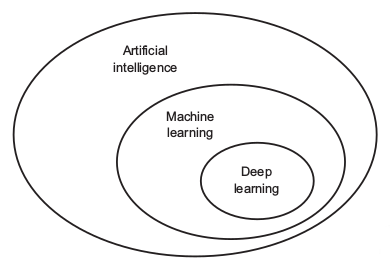
\includegraphics[width=0.5\textwidth]{imgs/marcoteorico.png}
\caption{Inteligencia Artificial, Aprendizaje Automático y Aprendizaje Profundo. \cite{Cho17}}
\end{figure}

\subsection{Inteligencia artificial}

En 1956, los padres de la \textit{Inteligencia Artificial}: Allen Newell, Herbert Simon, John McCarthy, Marvin Minsky y Arthur Samuel acuñaron el término \textit{``Inteligencia Artificial''} como \textit{``una rama de las Ciencias de la Computación que tiene como objetivo simular comportamiento inteligente en una computadora.''} \cite{ensayo-samuel} \cite{allen-newell}

En un principio dichos sistemas estaban dotados de una gran cantidad de reglas que los hacían muy efectivos para resolver ciertos problemas donde los pasos están bien definidos y son lógicos.

Entre las décadas del ’50 y ’80 se creyó que con un conjunto suficientemente grande de reglas se podría lograr una inteligencia al nivel de los humanos. 
No obstante ciertos problemas como el reconocimiento de objetos en imágenes o de transcripción de texto a partir de sonido son difíciles de tratar con este enfoque, a pesar de que los humanos lo pueden realizar sin dificultad. Y esencialmente la dificultad de estos problemas radica en que es complejo obtener un conjunto de reglas o pasos algorítmicos para resolverlos.

\subsection{ Aprendizaje automático } \label{aprendizaje-automatico}

En 1962 Arthur Samuel en su ensayo \textit{``Artificial Intelligence: A Frontier of Automation''} \cite{ensayo-samuel} propone construir algoritmos donde el flujo del programa dependa de ciertos pesos asignados por un mecanismo en función de la \textit{performance} calculada, de modo que las máquinas ``aprendan'' de su experiencia. 
Éste fue un puntapié inicial para la fundación del campo del \textit{aprendizaje automático}, el cual consiste en el estudio de algoritmos que mejoran automáticamente su rendimiento gracias a la experiencia.

\begin{figure}[h]
\centering
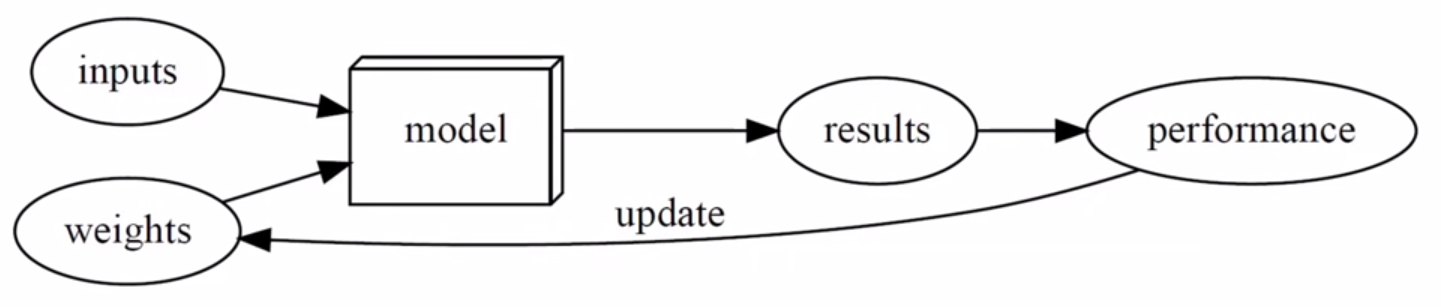
\includegraphics[width=1\textwidth]{imgs/automated-learning.png}
\caption{ Esquema de la estructura propuesta por Arthur Samuel. \cite{fastbook}}
\end{figure}

Tom Mitchell define en su célebre libro
 \textit{``Machine learning''} (1997, \cite{mitchell}) al aprendizaje automático como:

\begin{quote}
``Se dice que un programa de computadora aprende de la experiencia $E$ respecto a una tarea $T$ y una medida de desempeño $P$ , si el desempeño medido con $P$ en una tarea $T$ , mejora con la experiencia $E$.''
\end{quote}

De este modo los algoritmos de aprendizaje automático construyen un modelo con el objeto de realizar predicciones o tomar decisiones sin haber sido expresamente programados para hacerlo.
El modelo es construido en base a entradas suministradas. \\

La flexibilidad de las técnicas han ido aumentando y actualmente se pueden aplicar a gran variedad de problemas como reconocimiento de imágenes, sonidos, generación de texto, entre otros.
%\subsubsection{Clasificaciones dentro del Aprendizaje Automático}
\\
Dependiendo del tipo de experiencia suministrada se suele distinguir entre distintos problemas de aprendizaje \cite{rusell}:
\begin{itemize}
    \item \textbf{Supervisado:} se suministran los resultados esperados para las entradas ejemplo. El objetivo del modelo es ``aprender'' la relación entre las entradas y las salidas de modo que frente a nuevas entradas produzca razonables resultados. Es por ello que a menudo a estos últimos se los llamará también \textit{predicciones}.
    \item \textbf{No supervisado:} sólo hay entradas (no hay salidas) y el objetivo es entender la estructura fundamental de los datos y aprender relaciones ocultas importantes.
\end{itemize}

Dependiendo de las predicciones del modelo en el caso supervisado hablaremos de:
\begin{itemize}
    \item \textbf{Regresión:} si las predicciones son valores continuos.
    \item \textbf{Clasificación:} Si las predicciones pertenece a un dominio de valores discreto.
    A su vez hablaremos de \textit{clasificación binaria} si las predicciones poseen sólo dos valores posibles.
\end{itemize}

En el presente trabajo trataremos un problema de clasificación binaria mediante \textit{aprendizaje supervisado}.

\subsection{Terminología del Aprendizaje Automático}

En esta sección veremos con más formalidad los conceptos que atañen al \textit{Aprendizaje Automático}. Además introduciremos la jerga específica utilizada en el mismo. Una vez leídas todas las definiciones recomendamos volver a la sección \ref{aprendizaje-automatico} (\textit{``Aprendizaje Automático''}) para constatar que detrás de la rigurosidad de símbolos y terminología específica se esconde sencillamente el modelo imaginado por Arthur Samuel en 1962. \cite{ensayo-samuel} \\

Como se aclaró en la sección anterior, en el presente trabajo trabajaremos con un problema de aprendizaje supervisado. En dichos problemas tenemos un conjunto de ejemplos $D$ formado por entradas para las cuáles poseemos una (única) salida conocida. A este conjunto se lo denomina \textbf{conjunto de datos} (o \textbf{\textit{dataset}}):
\begin{equation*}
    D = \{ (x, y) \} \quad D \subset A \times B,
\end{equation*}
donde $x$ es un vector real de $p$ dimensiones ($x \in \mathbb{R}^p$) llamado \textbf{variable independiente} o  \textbf{vector  de características}. A cada componente del mismo se lo llama \textbf{característica} (o \textit{\textbf{feature}}).
%    $A$ será el subconjunto de posibles valores válidos de nuestra variable independiente: $A \subseteq \mathbb{R}^p$.
Por otro lado, $y$ es llamada \textbf{variable dependiente u objetivo} (o \textit{\textbf{target}}). En caso de tratarse de un problema de regresión $y$ es una variable continua ($B \subseteq \mathbb{R} $). Si tenemos un problema de clasificación se la llama también \textbf{etiqueta} (o \textit{\textbf{label}}). En este caso $B$ será el conjunto de clases posibles ($|B| \in \mathbb{N} $). Por ejemplo, $B = \{``gato'', ``perro''\}$ para un clasificador que distinga fotografías de gatos y perros. \\
    
    
Llamaremos $I$ al conjunto de todas las entradas y salidas posibles para nuestro problema. $I$ generalmente es infinito puesto que todas las posibles entradas $A$ suele ser infinito:

\begin{equation*}
    I = A \times B.
\end{equation*}

Volviendo al problema de clasificar imágenes de gatos y perros, $A$ sería el conjunto (infinito) de todas las posibles imágenes que sean razonables recibir para dicho clasificador (imágenes donde haya algo discernible como gato o perro). A su vez, $I$ será el conjunto de dichas imágenes junto su respectiva etiqueta.\\

Generalmente $D$ es finito ($|D| \in \mathbb{N} $) ya que son los datos que poseemos (para los cuales conocemos certeramente una relación entre una entrada y su esperada salida). En este caso el conjunto de entradas disponibles $D$ no es exhaustivo y existen muchas otras entradas factibles desconocidas que constituyen el \textbf{espacio problema}:
\begin{equation*}
    D \subset I.
\end{equation*}

En una aplicación real, los casos futuros a clasificar serán elementos de $I - D$.\\

El objetivo del problema es ``aprender'' una función $f : A \rightarrow B$ que le asigna a cada entrada una salida. El objetivo no es sólo que prediga bien $D$ sino que posea una buena \textbf{generalización} al espacio problema $I$.\\

Como el conjunto de datos no es exhaustivo ($I - D \neq \emptyset$). Y existen infinitas entradas que no aparecen en el conjunto de datos, luego existen infinitas $f$ consistentes con los datos (que los interpolan):
\begin{equation*}
    \mathbb{H} = \{ f~|~f(x)=y ~\forall (x,y) \in D \}
\end{equation*}
%Todo punto no perteneciente a $D_t$ tiene la misma probabilidad para cualquier valor de predicción posible:
%\begin{equation*}
    %P( \hat{f}(x)=y~|~D_t ) = P( \hat{f}(x)=y'~|~D_t ) ~ con ~ %x \notin D_t~ \forall y,y' \in B
%\end{equation*}
Es por ello que debemos descartar algunas hipótesis, para lo cual se hacen suposiciones de la solución. Esto constituye lo que se llama \textbf{sesgo inductivo} o \textbf{base inductiva}.  \\

Por ejemplo podemos hipotetizar que $f$ es una combinación lineal de las características:
\begin{equation*}
    f(x) = \sum_{i=1}^n c_i . x_i 
\end{equation*}

Nuestro \textbf{modelo} lo constituirán tanto dicha fórmula (producto de nuestras asunciones) como los valores de los coeficientes. 

Las predicciones del modelo dependerán de la elección de dichos coeficientes, también denominados \textbf{parámetros} o \textbf{pesos} (o \textbf{\textit{weights}}). Para encontrar valores adecuados para los parámetros se utiliza un \textbf{algoritmo de optimización}, teniendo en cuenta un subconjunto $D_t$ de los datos disponibles $D$ ($D_t \subset D$). Esto es lo que se conoce como \textbf{fase de aprendizaje}. Durante este proceso se habla de \textbf{ajuste de los datos de entrenamiento}, \textbf{ajuste de los pesos} o simplemente \textbf{ajuste del modelo}. A $D_t$ se lo llama \textbf{conjunto de entrenamiento}. A continuación veremos por qué es importante no utilizar la totalidad de los datos disponibles para ajustar los pesos. \\

También, deberá existir una manera de medir la performance del modelo a partir de los resultados del mismo y de entradas y salidas conocidas. A esto se lo denomina \textbf{métrica}: es una función de las \textbf{etiquetas} y \textbf{predicciones}.
\begin{equation*}
    metric( f(x), y )
\end{equation*}

El objetivo del modelo es tener una buena performance sobre todo el conjunto de entrada $I$. Como se dijo, en la práctica los casos de $I-D$ pueden ser casos futuros sobre los que se utiliza el modelo para tomar decisiones en función de las predicciones.

Es muy importante contar con ejemplos adicionales $D_v$ para los cuales se conozcan tanto entradas como salidas ($D_v \subset D$) y que no pertenezcan al conjunto que se utilizó para el ajuste del modelo ($D_t \cap D_v = \emptyset$). De modo que midiendo en $D_v$ la performance podamos cuantificar la \textbf{capacidad de generalización} del modelo, entendiéndose a esta como la capacidad de extrapolar los resultados de $metric$ a casos nos vistos durante el entrenamiento.

A dicho conjunto $D_v$ lo denominamos \textbf{conjunto de validación}. 
Si el conjunto de validación ha sido bien elegido (más adelante veremos que $D_t \cap D_v = \emptyset$ es condición necesaria pero no siempre suficiente) las métricas calculadas en dicho conjunto serán una buena estimación de las métricas esperadas en el resto de los casos no observados:
\begin{equation*}
    \mathbb{E}_{(x,y) \in D_v} [metric(f(x),y)]  \approx \mathbb{E}_{(x,y) \in E} [metric(f(x),y)]
\end{equation*}
Trasladado a un ejemplo práctico, esto quiere decir que nos dará una pauta confiable de la performance de nuestro modelo en la aplicación final. Es por ello que crear de forma correcta el conjunto de validación es crítico. La etapa de medir la performance del modelo sobre $D_v$ suele llamarse \textbf{fase de evaluación}.\\

Las elecciones que constituyen la base inductiva del modelo (elección del modelo, variables de configuración del mismo, estrategias de entrenamiento, etc) constituyen ``parámetros que actuarán sobre los parámetros del modelo''. Es por ello que estas elecciones son denominadas \textbf{hiperparámetros}. Éstos no son modificados (o \textit{ajustados}) por medio del mecanismo de optimización que actúa sobre los pesos, pero a menudo se prueban diferentes valores de hiperparámetros (entrenando diferentes modelos) y se elige el que tenga mayor performance en la fase de evaluación. Al usar el conjunto de validación de este modo el modelo finalmente elegido deja de ser independiente del conjunto de validación, por lo que se suele realizar una evaluación final sobre un tercer conjunto $D_h$ ($D_h \subset D$ y disjunto respecto $D_t$ y $D_v$) denominado \textbf{conjunto de test} para obtener la métrica de generalización del resultado final. \\

Es frecuente denominar \textbf{conjunto de desarrollo} a la unión del conjunto de entrenamiento y el conjunto de validación ($D_t \cup D_v$). El nombre proviene de que estos datos se utilizan durante el \textit{desarrollo} de la solución: el conjunto de entrenamiento para ajustar los parámetros del modelo y el conjunto de validación para elegir los hiperparámetros. El conjunto de test, en cambio, se reserva exclusivamente para la evaluación final y no debe influir en ninguna decisión de diseño.\\

Luego de evaluado un modelo, está en condiciones de utilizárselo en la aplicación final. La acción de aplicar el modelo a un ejemplo al cuál no se conoce su resultado suele denominarse \textbf{inferencia}.

\subsection{Dilema sesgo-varianza y sobreajuste}

Sea:
\begin{itemize}
    \item $Y$ la variable dependiente a predecir.
    \item $X$ los atributos (variable independiente) en los que se basa la predicción.
    \item $f$ la función a predecir (relación subyacente entre $X$ e $Y$).
    \item $\epsilon$ el ruido en los datos, distribuido normalmente con media $0$ y varianza $\sigma$
\end{itemize}
Tenemos la fórmula:
\begin{equation*}
    Y = f(X) + \epsilon
\end{equation*}
Sea $f$ el modelo que intenta aproximar $f$, el error cuadrático de predicción para un ejemplo $x$ resulta ser:
\begin{equation*}
    Error(x) = \mathbb{E}[(Y - f(x))^2]
\end{equation*}

En \cite{Hastie} se definen:
\begin{equation*}
    Sesgo = \mathbb{E}[f(x)] - y]
\end{equation*}
\begin{equation*}
    Varianza = \mathbb{E}[~(f(x) - \mathbb{E}[f(x)])^2~]
\end{equation*}
\begin{equation*}
    ErrorIrreducible = \sigma
\end{equation*}

Reescribiendo la fórmula del error como:
\begin{equation*}
    Error(x) = Sesgo^2 + Varianza + ErrorIrreducible
\end{equation*}
En donde cada término del error puede ser interpretados como causas diferentes del mismo. 

Haciendo un análisis de la composición del error, interpretando cada causa:
\begin{itemize}
    \item \textbf{Error irreducible}: producto de la varianza en la función que se quiere predecir, ruido en los datos, etc. Está fuera de nuestro control.
    \item \textbf{Sesgo}: diferencia entre la predicción promedio de nuestro modelo, y el valor correcto que intentamos predecir. Puede ser pensado como el error causado por asunciones simplistas del modelo, como por ejemplo tomar que la distribución de los datos es lineal.
    \item \textbf{Varianza}: es la variabilidad de la predicción de un modelo, es decir, cuánto varía $f(x)$ alrededor de su media. Modelos con alta varianza ``prestan mucha atención'' a los datos de entrenamiento, corriendo el riesgo de no generalizar tan bien en datos no incluidos en el entrenamiento.
\end{itemize}

Cuando ajustamos los datos de entrenamiento con mayor precisión correemos el riesgo de que el modelo se adapte demasiado a los datos de entrenamiento, y no generalice bien en los datos de validación. Este escenario es denominado \textbf{sobreajuste} (o \textit{\textbf{overfitting}}). Cuando esto ocurra, las métricas mostrarán mucho peores resultados en el conjunto de validación que en el de entrenamiento.

En contraste si no se ajusta lo suficiente a los datos de entrenamiento poseerá un alto sesgo. Esto es lo que se conoce como \textbf{subajuste} (o \textit{\textbf{underfitting}}). A diferencia del sobreajuste, en este caso el error se manifestará tanto en la validación como en el entrenamiento.

\begin{figure}[H]
\centering
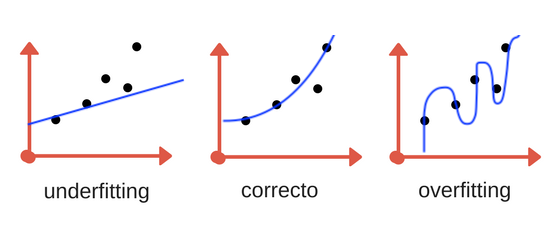
\includegraphics[width=0.85\textwidth]{imgs/overfitting.png}
\caption{ La imagen esquematiza que la elección de una base inductiva demasiado simple y poco expresiva puede ser el origen de un sesgo alto.
A su vez, modelos complejos que se pueden ajustar demasiado a los datos de entrenamiento pueden generar sobreajuste.}
\end{figure}

Es por ello que los modelos más complejos, al tener más capacidad expresiva, pueden ajustar mejor los datos de entrenamiento (y potencialmente sobreajustar). El error de entrenamiento tiende a decrecer cuando incrementamos la complejidad del modelo.

\begin{figure}[H]
\centering
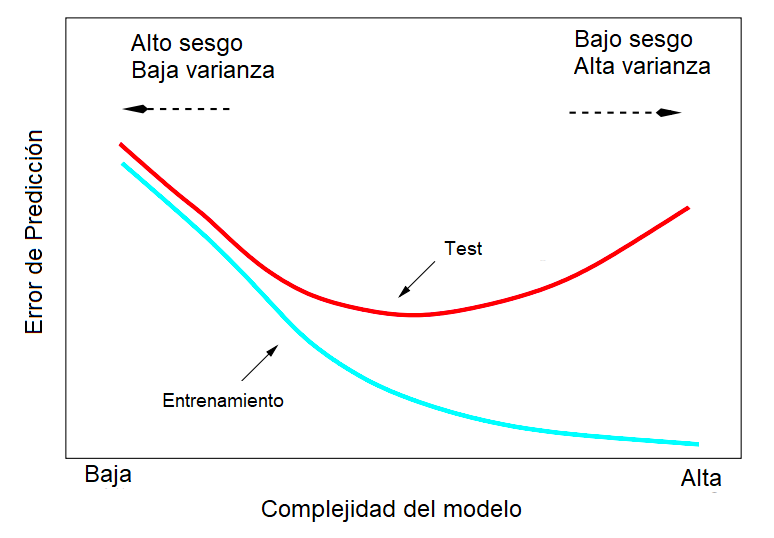
\includegraphics[width=0.95\textwidth]{imgs/complejidad-error.png}
\caption{ La gráfica esquematiza que cuando la complejidad de nuestro modelo crece, la varianza tiende a aumentar en tanto que el sesgo disminuye. Lo opuesto sucede cuando la complejidad del modelo disminuye. \cite{Hastie}}
\end{figure}

Esto último no quiere decir que siempre la primer solución al sobreajuste sea reducir la complejidad del modelo. Como dijimos, esta última aumenta la capacidad expresiva y por ende la \textit{capacidad} de sobreajustar. No obstante en métodos de optimización iterativos (como el empleado con las redes neuronales) podemos controlar la cantidad de ajuste por medio del número de iteraciones. Ya veremos que existen formas de combatir el sobreajuste y entrenar modelos más robustos llamados \textit{técnicas de regularización}.

Más adelante veremos que reducir la complejidad de los modelos ante la presencia del sobreajuste no es -generalmente- la mejor opción en el caso del Aprendizaje Profundo. De hecho, la práctica demuestra que es la última de las opciones a intentar entre un gran abanico de soluciones. Como veremos en la subsección \ref{subsection:representaciones}, en el aprendizaje profundo la gran complejidad de los modelos es lo que permite aproximar funciones complejas que reciban los \textit{``datos crudos''} (por ejemplo valores de píxeles en caso de imágenes) y calculen las representaciones idóneas para el proceso de clasificación. Esto constituye el gran éxito del aprendizaje profundo por sobre anteriores enfoques que consistían en extraer características con algún algoritmo \textit{ad-hoc} específico al dominio y tan solo luego utilizar un clasificador de aprendizaje automático.

El sobreajuste afecta a la mayoría de los métodos de Aprendizaje Automático. Es importante por ello contar con un conjunto de validación para medir las métricas elegidas en datos que no se usaron para entrenar.

\subsection{Conjunto de validación}

Como se dijo en secciones anteriores, se utiliza un \textbf{conjunto de datos de validación} $D_v$ no incluídos en el entrenamiento para medir la capacidad de generalización del modelo. 

Ya que nuestro objetivo final es aplicar el modelo en datos nunca antes vistos, $D_v$ debe ser representativo del conjunto de entradas factibles $E$.

De manera obvia, los datos de validación deben no aparecer entre los datos de entrenamiento $D_t$:
\begin{equation*}
    D_v \cap D_t = \emptyset
\end{equation*}
A menudo se toma una partición aleatoria de los datos. Pero también debe evitarse cualquier correlación con los datos de entrenamiento $D_t$ que no sea extensible al conjunto de entradas factibles $E$.

 Un ejemplo dónde, claramente, no es válido partir aleatoriamente las entradas para construir los conjuntos de entrenamiento y validación es las series temporales (véase figura \ref{fig:validacion-ts}). De hacerlo es fácil para el modelo aprender valores certeros teniendo valores conocidos durante el entrenamiento dentro del entorno cercano del valor a predecir. Contrariamente a este escenario, en una aplicación real probablemente querramos predecir valores \textit{futuros}. Por lo que una correcta partición tomaría un rango continuo de los últimos valores para confeccionar un conjunto de validación representativo.\\

Al ser un punto tan crítico la creación de un buen conjunto de validación suele ser fuente de numerosos errores en aplicaciones prácticas.

\begin{figure}[H]
\begin{subfigure}{0.33\textwidth}
\centering 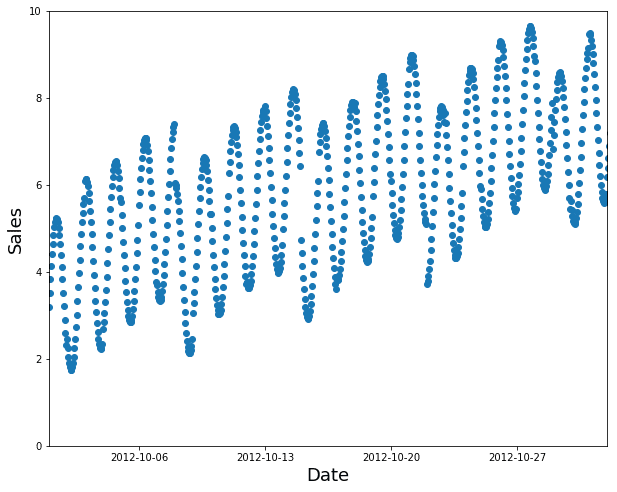
\includegraphics[width=0.3\textwidth]{imgs/ts11.png}
\end{subfigure}
\begin{subfigure}{0.33\textwidth}
\centering 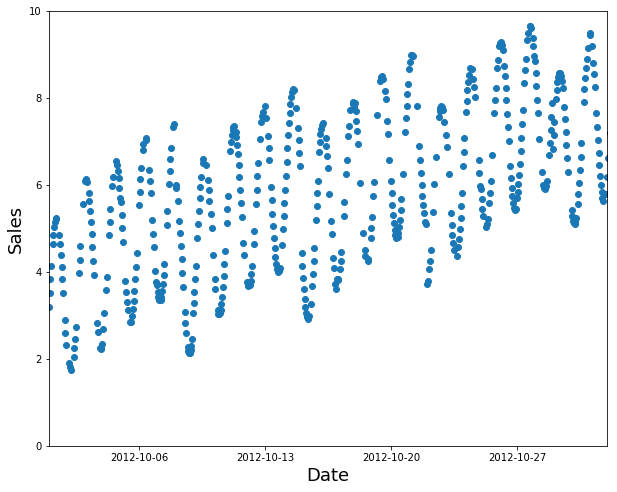
\includegraphics[width=0.3\textwidth]{imgs/ts2.png}
\end{subfigure}
\begin{subfigure}{0.33\textwidth}
\centering 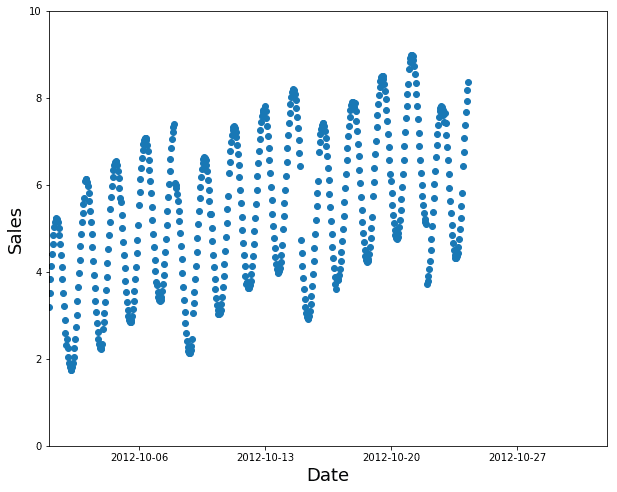
\includegraphics[width=0.3\textwidth]{imgs/ts3.png}
\end{subfigure}
\caption{ La primer figura muestra una serie temporal. La segunda muestra un subconjunto aleatoriamente seleccionado de ejemplos. La última muesta un subconjunto de entrenamiento correctamente seleccionado: siendo la validación un rango continuo de los últimos valores.  Fuente: \cite{fastai-validation} }
\label{fig:validacion-ts}
\end{figure}

En conjuntos de datos académicos es frecuente que la separación en conjunto de validación ya esté dada con el mismo conjunto para que los resultados de diversas investigaciones sean comparables de forma correcta.\\


\subsubsection{Validación cruzada}

El método de validación cruzada (descripto en \cite{berrar}) consiste en entrenar y evaluar modelos sobre diferentes particiones de entrenamiento y validación y combinar los resultados de los valores de las métricas obtenidos (por ejemplo tomando el promedio).

Existen diferentes estrategias de validación cruzada:
\begin{itemize}
    \item \textbf{K-iteraciones} (o \textit{K-folding}): consiste en particionar los datos disponibles en $k$ grupos y hacer $k$ iteraciones. En la $i$-ésima se utiliza el grupo $i$ para validación y el resto se lo usa para entrenamiento.
    \item \textbf{Aleatoria}: consiste en hacer $k$ iteraciones donde se elijen aleatoriamente la partición de validación. Como ventaja el tamaño de la partición no depende del número de iteraciones. Dentro de las desventajas destaca que existe la probabilidad de que existan ejemplos que no sean incluídos en ninguna validación.
    \item \textbf{Dejando uno afuera}: consiste en hacer $N$ iteraciones (siendo $N$ la cantidad de muestras disponibles). En la $i$-ésima iteración se utilizan todos los datos para entranar excepto el $i$-ésimo elemento del conjunto que se usa para evaluación.
\end{itemize}

\begin{figure}[h]
\centering
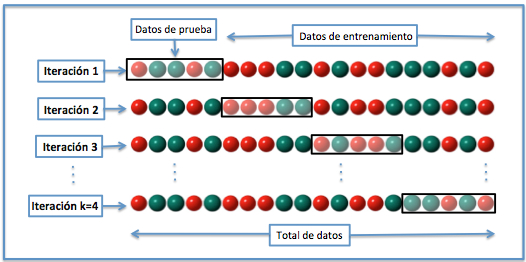
\includegraphics[width=1\textwidth]{imgs/Kfold_cross_validation.jpg}
\caption{Método de validación cruzada de K-iteraciones. Fuente: \cite{image-cross-validation}}
\end{figure}

La limitación de la validación cruzada es el gran esfuerzo computacional. Esto es debido a que se deben ejecutar $k$ entrenamientos independientes. 

Por lo que se utiliza validación cruzada mayormente cuando se cuenta con pocos datos. Es muy útil, también, en casos donde el puntaje de validación suele no ser preciso debido a que varía demasiado al cambiar la partición de validación elegida (generalmente sucede cuando se posee pocos datos y el conjunto de validación es demasiado pequeño). Así, eligiendo diferentes particiones y promediando el puntaje, se obtiene un estimador de menor varianza del puntaje real o de generalización.

Un dato importante a tener en cuenta es que muchos esquemas de validación cruzada son sólo aplicable cuando uno puede particionar aleatoriamente los datos para obtener un conjunto de validación representativo.


\subsection{Elección de hiperparámetros}

Como se mencionó en anterioremente, generalmente se exploran diferentes elecciones de hiperparámetros. A este procedmiento a veces se lo conoce como \textbf{puesta a punto del modelo} o \textit{\textbf{model tunning}} (no confundir con \textit{fine tunning} que es la técnica de re-utilizar un modelo ya entrenado en otros conjuntos de datos, explicado más adelante en el trabajo).

Existen diferentes estrategias para la exploración de hiperparámetros tales como:
\begin{itemize}
    \item \textit{\textbf{Grid Search:}} se prueban todas las asignaciones posibles para conjuntos de valores propuestos para cada hiperparámetro.
    \item \textit{\textbf{Random Search:}} se prueban asignaciones aleatorias de los hiperparámetros dentro de un conjunto de valores propuestos para cada uno.
    \item \textbf{Optimización Bayesiana:} utiliza el método bayesiano de optimización global para maximizar funciones (para una descripción detallada ver \cite{bayesian}). Suele obtener mejores resultados que el \textit{Random Search} y requerir menor cómputo que \textit{Grid Search} por su capacidad de razonar acerca de las asignaciones que no han sido probadas, y así elegir cuáles probar.
    \item \textbf{Algoritmos genéticos:} parten de un conjunto de asignación inicial y genera otras cambiando aletoriamente algunos valores de hiperparámetros. Luego de cada paso se queda con las mejores asignaciones (de mayor performance).
    \item \textbf{Manualmente:} En la práctica suele ser poco factible entrenar el modelo varias veces para demasiadas asignaciones de hiperparámetros. Esto es especialmente cierto en el \textit{aprendizaje prufundo} donde el tiempo de entrenamiento es considerable.
    Comúnmente se prueban manualmente hiperparámetros que son conocidos en la literatura que funcionan bien por defecto. 
\end{itemize}

En general métodos exhaustivos como \textit{Grid Search} no se utilizan en la práctica por la demanda de tiempo que conlleva. Se suele ver en la literatura científica y sólo tienen sentido si se desea arribar a conclusiones sobre determinados hiperparámetros (también es visto su uso en \textit{competencias de modelos} donde diferencias mínimas en la performance permiten escalar en la tabla de posiciones).

Frecuentemente también se utilizan métricas y visualizaciones para analizar la estabilidad del entrenamiento, convergencia del proceso de optimización y otras heurísticas, por medio de las cuales podemos estimar si es necesario variar determinado hiperparámetro. 

En el Capítulo 6 de FastBook \cite{fastbook}, por ejemplo, se explica cómo elegir el umbral de aceptación para un problema de clasificación multicategoría dónde la salida del modelo son probabilidades. Para ello se visualiza cómo varía la tasa de aciertos (calculada en el conjunto de validación) para diferentes valores del umbral (ver figura \ref{fig:umbralacc}).
Ahí mismo se explica que, como \textit{''regla heurística''} general, cuándo se eligen hiperparámetros de este modo raramente se estará sobreajustando el conjunto de validación si la gráfica de la métrica en función del hiperparámetros es suave.\\

\begin{figure}[h]
\centering
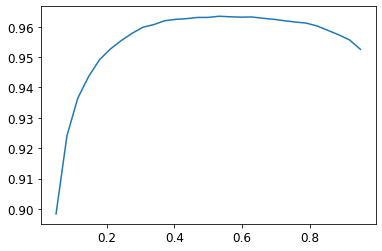
\includegraphics[width=0.8\textwidth]{imgs/accuracy_umbral.png}
\caption{ Tasa de aciertos en función al umbral de aceptación elegido para un problema de clasificación multi-categoría. Fuente: \cite{fastbook}.  }
\label{fig:umbralacc}
\end{figure}

Veremos más adelante en el presente trabajo algunas técnicas populares en la práctica del aprendizaje profundo que se utilizan a menudo para elegir manualmente hiperparémetros, incluso en circunstancias como competencias de modelos dónde hilar fino en las métricas es muy importante.
    

\subsection{Conjunto de test}

Las diferentes asignaciones de hiperparámetros son comparadas teniendo en cuenta las métricas sobre el conjunto de validación. Si se realizan demasiadas pruebas se corre el riesgo de ``sobreajustar los hiperparámetros'' y  que la performance que guia la elección de los mismos no generalice bien a conjuntos de datos no observados.\\

Como se explicó en secciones anteriores, se suele contar con un tercer conjunto de datos (además del de entrenamiento y de validación) denominado \textbf{conjunto de test}. El mismo se utiliza para realizar una evaluación final no sesgada del modelo. Ésto puede parecer un despropósito pero es necesario para seguir una metodología correcta y mantenernos intelectualmente honestos.\\

\subsection{Métricas} \label{ref:metrics}

Ya hemos introducido el concepto de \textbf{métricas} en las secciones anteriores donde explicamos que son funciones para medir la performance del modelo.

Las \textbf{metricas} (pueden considerarse varias) son problema-dependientes debido a que dependen tanto de la naturaleza de las predicciones y de las entradas como del objetivo para el cuál se utilizará el modelo. 

Deben poseer un significado interpertable por los usuarios en términos del uso que se le está dando al modelo.

No se debe confundir métrica con la \textit{función de costo} que utiliza el mecanismo automático de optimización del modelo y a menudo posee propiedades matemáticas deseables por el mismo. El concepto se tratará más detalladamente cuando se hable de descenso por gradiente en redes neuronales  (subsección \ref{subsection:descenso-gradiente}).

\subsubsection{Métricas en problemas de regresión}
En problemas de regresión podemos encontrar las métricas:
\begin{itemize}
    \item \textbf{Error cuadrático médio (MSE):} es una de las métricas más utilizadas en problemas de regresión puesto a qué es una función diferenciable. Pero penaliza los errores grandes, siendo suceptible a valores atípicos.
    \begin{equation*}
        MSE = \frac{1}{n} \sum_{i=1}^n ( y_i - \hat{f}(x_i) )^2
    \end{equation*}
    \item \textbf{Error absoluto médio (MAE): } no penaliza tanto a los errores grandes como MSE.
    \begin{equation*}
        MAE = \frac{1}{n} \sum_{i=1}^n | y_i - \hat{f}(x_i) | 
    \end{equation*}
    \item \textbf{Coeficiente de determinación ($R^2$)}: representa que proporción de la varianza de la variable dependiente $y$ es explicada por las características de la variable independiente $x$.
    \begin{equation*}
        R^2 = 1 - \frac{\sum_{i=1}^n ( y_i - \hat{f}(x_i) )^2}{\sum_{i=1}^n ( y_i - \overline{y} )^2} 
    \end{equation*}
    También puede ser pensada como una comparación del MSE de nuestro modelo con el del \textit{baseline} trivial de predecir la media de las entradas.
\end{itemize}

\subsubsection{Métricas en problemas de clasificación}
En problemas de clasificación podemos encontrar las métricas:
\begin{itemize}
    \item \textit{\textbf{Accuracy}} es una de las métricas más utilizadas en problemas de clasificación. Consiste simplemente en la proporción de aciertos realizados. También se la conoce como \textbf{tasa de aciertos}.
    \begin{equation*}
        Accuracy = \frac{1}{n} \sum_{i=1}^n Igual( y_i, \hat{f}(x_i) )
    \end{equation*}
    \begin{equation*}
        Igual(a,b) = \left\lbrace\begin{array}{c} 1~si~a = b \\  0~si~a \neq b \end{array}\right.
    \end{equation*}
    \item \textit{\textbf{Top k - Accuracy:}} para problemas donde el número de clases es grande y existen varias fácilmente confundibles entre sí usualmente se modifica el problema de clasificación permitiendo a la predicción ser un conjunto de $k$ elementos (para cierto $k$ fijo) y se mide como acierto si la clase objetivo pertenece a este conjunto de predicciones.
    \begin{equation*}
        Top~k-Accuracy = \frac{1}{n} \sum_{i=1}^n Acierto( y_i, \hat{f}(x_i) )
    \end{equation*}
    \begin{equation*}
        Acierto(etiqueta, predicciones) = \left\lbrace\begin{array}{c} 1~si~etiqueta \in predicciones \\  0~si~etiqueta \notin predicciones \end{array}\right.
    \end{equation*}
    \item \textbf{Matriz de confusión:} a menudo resulta útil calcular una matriz donde los ejes sean las etiquetas y las predicciones. De modo de contener en la casilla $M_{i,j}$ cuántos ejemplos de la clase $i$ han arrojado como resultado una predicción para la clase $j$.
    Los elementos de la diagonal representan los aciertos, mientras que los otros muestran errores.
    Es utilizada también debido a que confundir una clase por otra puede tener diferentes consecuencias prácticas y por lo tanto se puede preferir cierto tipo de errores a otros. Para comparar dos resultados y determinar cuál es mejor se pueden utilizar matrices de ponderación que le asignen a cada $M_{i,j}$ un costo $C_{i,j}$ ($C_{i,i} = 0$) de modo que el error quede definido como:
    \begin{equation*}
        Error = \sum_{i}\sum_{j}M_{i,j} \times C_{i,j}
    \end{equation*}
    De modo que $C_{i,j}$ refleje el costo práctico de cada tipo de error.
\end{itemize}

\begin{figure}[h]
\centering
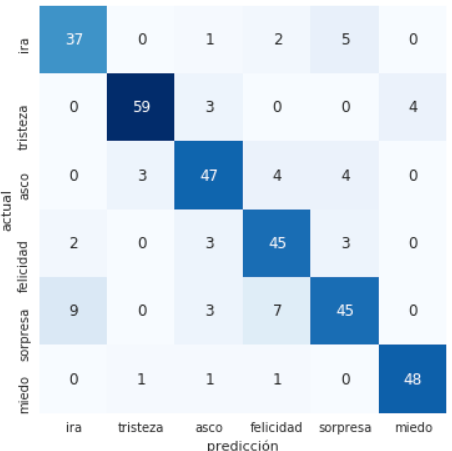
\includegraphics[width=0.45\textwidth]{imgs/confusion-matrix.png}
\caption{Ejemplo de una matriz de confusión para un problema de detección de emociones de 6 clases.}
\end{figure}

Dependiendo de la aplicación podemos querer optimizar diferentes métricas (y a menudo hay un \textit{trade-off} entre ellas). Por ejemplo en un problema de clasificación binaria para detectar tumores querremos que no se le pase ningún tumor maligno como beningno, a costa de arrojar un número razonable de falsas alarmas.\\

Es importante \textbf{siempre calcular las métricas en el conjunto de validación}. Las métricas sobre el conjunto de entrenamiento tienen poco sentido, se monitorean con la única utilidad de detectar cuándo el modelo está sobreajustando.

\subsubsection{Métricas en problemas de clasificación binaria}
\label{subsubsection:metricbinary}

Como ya comentamos, en el presente trabajo trataremos un problema de clasificación binaria. Es por ello que haremos especial énfasis en las métricas que atañan a ésta subcategoría de problemas de clasificación. 

En esta subcategoría de problemas suele denominarse a las clases como \textbf{positiva} y \textbf{negativa} \cite{metricas-binarias}. La decisión de a cuál clase definir como positiva y a cuál definir como negativa a veces es clara como por ejemplo en problemas de detección: la clase positiva será la etiqueta \textit{detectado} y la negativa \textit{no detectado}.

En nuestro caso querremos detectar errores en la confección de telegramas, buscando detectar \textit{no coincidencias} de firmas. Por eso trataremos como positiva a las \textit{no coincidencias}, ya que son las clases que se utilizará para desencadenar alertas en el sistema al cuál se pretende integrar la detección. En otros casos como en el problema de \textit{``Verificación Automática de Firmas Manuscritas''} \cite{tesis-parodi} se pretende verificar que la autoría de cierta firma es la que declara ser, comparándola con las de un autor registrado al que se le conocen ciertas firmas auténticas. En dicho trabajo se trabaja como clase positiva a la verificación de una firma como auténtica, o sea cuando coincide con las registradas del autor que declara ser. Es importante tener esto en cuenta a la hora de comparar métricas entre diferentes trabajos e implementaciones. \\

Luego de definidas las clases como positivas y negativas las predicciones del modelo pueden clasificarse en cuatro categorías en relación a su valor y al de la etiqueta respectiva según:

\begin{table}[h!]
\begin{tabular}{l|c|c|l}
\cline{2-3}
\textbf{}                                        & \multicolumn{1}{l|}{\textbf{Predicción Positiva}}                 & \multicolumn{1}{l|}{\textbf{Predicción Negativa}}                 &  \\ \cline{1-3}
\multicolumn{1}{|l|}{\textbf{Etiqueta Positiva}} & \begin{tabular}[c]{@{}c@{}}$TP$\\ (Verdadero Positivo)\end{tabular} & \begin{tabular}[c]{@{}c@{}}$FN$\\ (Falso Negativo)\end{tabular}     &  \\ \cline{1-3}
\multicolumn{1}{|l|}{\textbf{Etiqueta Negativa}} & \begin{tabular}[c]{@{}c@{}}$FP$\\ (Falso Positivo)\end{tabular}     & \begin{tabular}[c]{@{}c@{}}$TN$\\ (Verdadero Negativo)\end{tabular} &  \\ \cline{1-3}
\end{tabular}

\caption{Las abreviaciones TP, TN, FP, FN son populares en la literatura y provienen de los nombres en inglés, respectivamente: \textit{True Positive}, \textit{True Negative}, \textit{False Positive} y \textit{False Negative} }
\end{table}

Definirimos también (para simplificar la notación en las fórmulas) las super-categorías (constituída por uniones de las cateogrías definidas):
\begin{itemize}
    \item \textbf{Etiqueta Positiva}: conjunto de los datos que pertenecen a la clase positiva.
    \begin{equation*}
        P = TP+FN
    \end{equation*}
    
    \item \textbf{Etiqueta Negativa}: conjunto de los datos que pertenecen a la clase negativa.
    \begin{equation*}
        N = TN + FP
    \end{equation*}
    
    \item \textbf{Totalidad de datos}: conjunto de todos los datos usados para la evaluación.
    \begin{equation*}
        Total = FP+FN+TP+TN
    \end{equation*}
\end{itemize}

Luego se definen en función de las cardinalidades de dichas categorías diversas métricas para el problema de clasificación binaria (veáse \cite{metricas-binarias}), cada una con implicancias y significados distintos:
\begin{itemize}
    \item \textbf{Tasa de aciertos} (o \textit{\textbf{accuracy}}): simplemente la proporción de ejemplos clasificados correctamente.
    \begin{equation*}
        Accuracy = \frac{TP+TN}{Total}
    \end{equation*}
    
    \item \textbf{Ratio de error} (o \textit{\textbf{error rate}}): es el concepto complementario al de tasa de aciertos, la proporción de errores cometidos.
    \begin{equation*}
        Error~Rate = \frac{FP+FN}{Total} = 1 - Accuracy
    \end{equation*}
    
    
    \item \textbf{Exhaustividad} (\textit{\textbf{recall}} o \textbf{TPR} \textit{True Positive Rate}): la proporción de ejemplo positivos detectados como tales.
    \begin{equation*}
    Recall = \frac{TP}{TP+FN} = \frac{TP}{P}
    \end{equation*}
    En términos de probabilidad puede ser interpretado como la probabilidad de que nuestro modelo detecte un caso positivo.
    
    \item \textbf{Ratio de falsos negativos} (o \textbf{FNR} \textit{False Negative Rate}): es el concepto complementario a \textit{recall}:
    \begin{equation*}
    FNR = \frac{FN}{TP+FN} = \frac{FN}{P} = Miss~Rate = 1 - Recall
    \end{equation*}
    Puede ser interpretado como la probabilidad de que el modelo falle al detectar casos positivos. Por ello también se lo llama \textit{Miss Rate}.
    
    
    \item \textbf{Especificidad} (\textbf{\textit{Specificity}} o \textbf{TNR} \textit{True Negative Rate}): la proporción de ejemplo negativos detectados como tales.
    \begin{equation*}
    Specificity = \frac{TN}{FP+TN} = \frac{TN}{N}
    \end{equation*}
    En términos de probabilidad puede ser interpretado como la probabilidad de que nuestro modelo detecte un caso negativo.
    
    \item \textbf{Ratio de falsos positivos} (o \textbf{FPR} \textit{False Positive Rate}): es el concepto complementario a \textit{especificidad}:
    \begin{equation*}
    FPR = \frac{FP}{FP+TN} = \frac{FP}{N} = False~Alerts = 1 - Specificity
    \end{equation*}
    Puede ser interpretado como la probabilidad de que el modelo falle al detectar casos negativos. Por ello también se lo llama \textit{Falsas Detecciones} o \textit{Falsas Alertas}.
    
    
    \item \textbf{Precisión} (\textit{precision} en inglés): es la proporción de detecciones (predicciones positivas) que son correctas.
    \begin{equation*}
    \text{Precisión} = \frac{TP}{TP+FP} = \frac{TP}{\text{Predicción~Positiva}}
    \end{equation*}
    Puede interpretarse como qué tan probable es que una alerta por clase positiva esté bien, por eso también se lo denomina \textbf{poder predictivo positivo}.
\end{itemize}

\subsubsection{Métricas en el problema de Verificación Automática de Firmas Manuscritas} \label{subsubsection:metricasfirmas}

En aplicaciones reales es importante conocer las implicancias prácticas de las métricas y definir objetivos razonables (no se suele desarrollar sin un objetivo ya que no se sabría cuándo considerar que el trabajo es suficientemente bueno). Los objetivos deben proveer garantías prácticas a los usuarios y dependerán del uso de la aplicación. Por ello, siempre hay que tener presente para qué se usará el modelo que pretendemos crear a la hora de elegir la métrica y qué significado nos provee dicha métrica. \\

En la bibliografía de \textit{``Verificación Automática de Firmas Manuscritas''} \cite{tesis-parodi} se trabaja con las métricas:
\begin{itemize}
    \item \textbf{Tasa de Falsos Rechazos (FRR)}: porcentaje o ratio de rechazos de firmas auténticas.
    \item \textbf{Tasa de Falsa Aceptación (FAR)}: porcentaje o ratio de aceptaciones de falsificaciones.
\end{itemize}

El punto donde son iguales se suele llamar Tasa de error de intersección o \textbf{\textit{Equal Error Rate} (EER)}. De tratarse de un dataset con clases balanceadas será igual a la tasa de aciertos (ver figura \ref{fig:err}). \\

\begin{figure}[h]
\centering
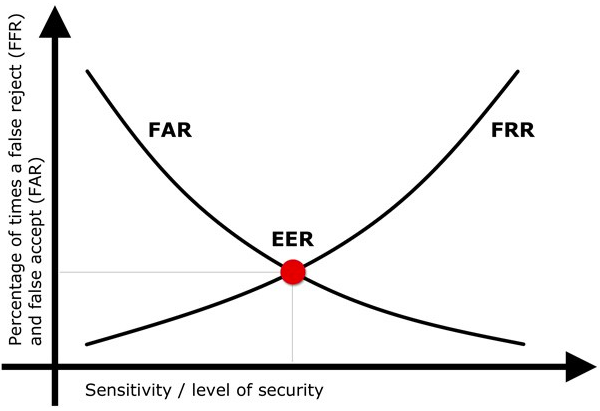
\includegraphics[width=0.5\textwidth]{imgs/err.png}
\caption{ La tasa de error de intersección es la elección del umbral de sensibilidad que representa un balance equitativo entre falsos positivos y falsos negativos. Créditos de la imagen: \href{https://www.recogtech.com/en/knowledge-base/security-level-versus-user-convenience}{\textit{``FAR and FRR: security level versus user convenience''} } }
\label{fig:err}
\end{figure}

No es lo mismo rechazar una firma auténtica que aceptar una falsificación. Por ejemplo en una aplicación de detección automática de fraude se querrá priorizar no aceptar falsificaciones a costa de a veces arrojar falsos rechazos. \\

Como \cite{tesis-parodi} toma como clase positiva las firmas auténticas (que son de quién declaran ser) resulta:

\begin{equation*}
        FRR = \frac{FN}{P}  = 1 - Recall
\end{equation*}
\begin{equation*}
    FAR = \frac{FP}{N} = FPR =  Falsas~Alertas 
\end{equation*}

En cambio, en nuestro problema particular tendremos pares de firmas y querremos saber si fueron hechas o no por la misma persona para detectar errores en la confección de los telegramas. En función de esto el sistema al cual se integrará el modelo levantará una alerta de posible error al usuario. Es por ello que, como se dijo en la sección anterior, trataremos como clase positiva a los pares de firmas \textit{no coincidentes}.
Bajo este enfoque las métricas nombradas para el problema de verificación automática de firmas se relacionan con las métricas del problema de clasificación binaria definido por nosotros de la siguiente manera:
\begin{equation*}
    FRR = Falsas~Alertas =  1 - Specificity
\end{equation*}
\begin{equation*}
    FAR = Miss~Rate = 1 - Recall.
\end{equation*}

\noindent Esto es consistente con que en nuestro sistema los rechazos (no coincidencias) generan alertas y las aceptaciones (coincidencias) dan lugar a la aprobación del telegrama.

\subsubsection{Análisis costo-beneficio para las métricas en clasificación binaria}
\label{subsubsection:costo-beneficio}

A menudo los métodos de aprendizaje automatizado para clasificación binaria producirán un puntaje o score entre $[ 0 , 1 ]$ para cada instancia a clasificar. Este puntaje suele ser interpretado como la certeza del modelo o probabilidad de la instancia de pertenecer a la clase positiva.
%\begin{equation*}
 %   score(x) \in [0, 1]
%\end{equation*}
Luego el modelo aplica un umbral elegido $t \in [0,1]$ para determinar la predicción:
\begin{equation*}
    model(x) = \left\lbrace\begin{array}{c} Prediccion~Positiva~si~score(x) > t \\  Prediccion~Negativa~si~score(x) \leq t \end{array}\right.
\end{equation*}

Valores altos de $t$ serán más conservadores a la hora de \textit{detectar}, y sólo clasificarán como positivos ejemplos para los cuáles estén muy seguros que lo son. Es por ello que al incrementar el umbral aumentaremos el \textit{precision}. Como contraparte al aumentar $t$ habrá potencialmente más ejemplos positivos mal clasificados (falsos negativos), o sea disminuirá el \textit{recall}.

Esta relación costo-beneficio entre \textit{precision} y \textit{recall} al variar el umbral de clasificación, también se evidencia entre \textit{recall} y \textit{False Alerts}: disminuyendo el umbral podemos hacer más propenso al modelo a clasificar una instancia como positiva aumentando la cantidad de positivos correctamente clasificados pero potencialmente aumentarán también las falsas detecciones.

Las relaciones de compromisos especificadas en párrafos anteriores admiten ser analizadas gráficamente: variando el valor del umbral $t$ se pueden obtener diferentes relaciones de compromiso entre las dos variables y obtener una gráfica 2D de una en función de la otra. Así se definen las curvas:
\begin{itemize}
    \item \textbf{Curva ROC} (por su nombre en inglés \textit{Receiver Operating Characteristic}) \cite{roc}: graficando los valores de \textit{Recall} y \textit{False Alerts}.  Se muestra un esquema de qué formas tienen las curvas en en la figura \ref{fig:roccurve}.
    \item \textbf{Curva DET} (por su nombre en inglés \textit{Detection Error Tradeoff}) \cite{det}: graficando los valores de \textit{miss rate} y \textit{falsas alarmas} y generalmente utilizando escala normal o logarítmica sobre ambos ejes. La información contenida es análoga a la de las curvas ROC debido a que el \textit{miss rate} es el concepto complementario a \textit{recall} pero la escala aplicada a los ejes hace que sean curvas más lineales y fáciles de analizar visualmente.
    \item \textbf{Curva Precision-Recall} \cite{desbalanceado}: graficando los valores de \textit{precision} en función del \textit{recall}. Se muestra un ejemplo en la figura \ref{fig:precisionrecall}. Como se explicará más adelante es muy popular analizar esta relación de compromiso especialmente cuando se trabaja con conjuntos de datos desbalanceados.
\end{itemize}

\begin{figure}[h]
\centering
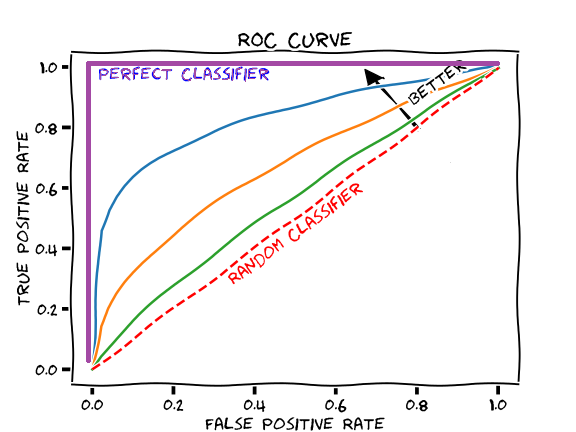
\includegraphics[width=0.6\textwidth]{imgs/roccurve.png}
\caption{ Figura esquemática donde ser observa como varían las curvas ROC de los modelos comparándolas con los casos extremos: el modelo de predicción aleatoria (peor modelo para la clasificación binaria) y el modelo ideal que siempre acierta. Créditos: The Machine Learners \url{www.themachinelearners.com/curva-roc-vs-prec-recall} }
\label{fig:roccurve}
\end{figure}

\begin{figure}[h!]
\centering
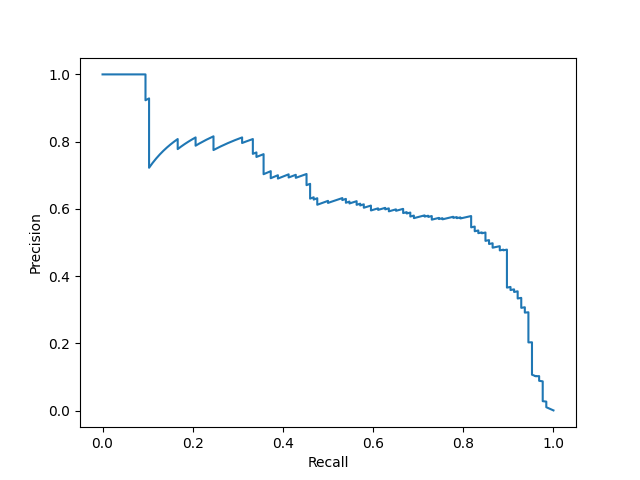
\includegraphics[width=0.6\textwidth]{imgs/precisionrecall.png}
\caption{Ejemplo de una curva de \textit{precision-recall}. Cada punto de la curva corresponde
a la \textit{precision} y el \textit{recall} obtenidos para un cierto valor de umbral de clasificación $t$.}
\label{fig:precisionrecall}
\end{figure}

La elección de métricas adecuadas es todavía más compleja en \textbf{problemas desbalanceados}, es decir, en problemas donde una de las dos clases es mucho más probable que la otra. Por ejemplo, en diagnóstico médico o detección de fraude, a menudo existen en el conjunto de datos un número pequeño de ejemplos clasificados como positivos. Esto puede acarrear que un modelo que se entrene para maximizar la \textit{tasa de aciertos} degenere en predecir siempre la clase más abundante (la negativa en los casos mencionados). No obstante, el \textit{miss rate} es crítico en los ejemplos nombrados: ¡significará fraude no detectado o patologías existentes no diagnosticadas!. \\

Existen técnicas para corregir manualmente el \textit{imbalance} de los datos como eliminar aleatoriamente parte de la clase mayoritaria (\textit{\textbf{undersampling}}) \cite{undersampling} o repetir instancias de clase minoritaria (\textit{\textbf{oversampling}}) \cite{oversampling} y técncias para que el clasificador pondere más una clase que otra \cite{desbalanceado}. 
Es de suma importancia tener en cosnideración que utilizar dichos métodos \textit{en la evaluación del modelo} muchas veces constituye un \textbf{error metodológico grave}: no se puede modificar el conjunto de datos de evaluación, ya que el mismo deberá poseer la misma distribución del hipotético conjunto de datos futuro sobre el que se aplicará el modelo (o sea, los datos que aparecerán en la aplicación final). Por ende deberán también poseer el mismo grado de \textit{imbalance}. Es por eso que las mencionadas técnicas suelen aplicarse sólo durante la fase de entrenamiento.

En éstos casos donde los datos son desbalanceados \textit{por naturaleza} lo que debemos adaptar es la estrategia de evaluación eligiendo métricas robustas al desbalance. Analizar \textit{precision} y \textit{recall} suele ser una buena opción ya que evaluaremos detectar una cierta proporción de la clase positiva pese a que sea pequeña (\textit{recall}) y tener cierta confianza en que las predicciones positivas son correctas (\textit{precision}). Para conjugar estas dos métricas y obtener una medida de perforcmance numérica es común calcular el área debajo de la curva \textit{Precision-Recall}, denominada \textbf{R-AUPRC}. Esta fórmula considera los valores de \textit{precision} y \textit{recall} para todos los valores de umbrales posibles. 

En la práctica generalmente se considera al umbral como parte del modelo final ya que son las predicciones las que se utilizarán para tomar decisiones. Una estrategia que tiene en cuenta ambas métricas a la hora de elegir el umbral  es pensar un umbral de \textit{recall} o \textit{precision} aceptado y maximizar la otra variable. 

En el caso de nuestros errores en telegramas electorales, una alerta de \textit{no coincidencia} (clase positiva) previene que se soliciten retransmisiones por telegramas mal confeccionados desde el centro de cómputo, lo cuál genera trabajo humano innecesario. Como estaremos satisfechos en reducir en $\times 5$ las retransmisiones, nos contentaremos con un \textit{recall} del $0.8$. A su vez, si el ratio de falsas alertas es alto, el usuario desestimará las alarmas, por lo que queremos que la \textit{precision} sea de al menos $0.95$ (de modo que a lo sumo $1$ de cada $20$ alarmas sean \textit{falsas alarmas}).

Puede ser interesante disponer de una forma de comparar dos modelos de predicción (habiendo fijado el umbral para cada uno). Para ello se suele combinar \textit{recall} y \textit{precision} en una única métrica utilizando el $\boldsymbol{F}$\textbf{\textit{-score}} (o $\boldsymbol{F}$\textbf{\textit{-measure}}), que es la media armónica de ambas:

\begin{equation*}
    F\text{-}score = \frac{2}{recall^{-1} + precision^{-1}} = 2 \frac{precision . recall}{precision + recall}
\end{equation*}

A veces los conjuntos de datos son generados y poseen desbalance. Ésto es algo que ocurre en los problemas de similitud que se discutirán más adelante en la tesina: generalmente poseemos varios ejemplos que pertenecen a diferentes clases (firmas de un mismo autor, caras de una persona, etc) y construimos nuestros conjuntos formando pares que constituyan \textit{coincidencias} y \textit{no coincidencias}. De este modo podemos correr el riesgo de generar conjuntos desbalanceados (por ejemplo si se toman todos los pares de elementos). En \cite{tesis-parodi} se nombra el problema de desbalanceo en los conjuntos de datos (generados como parte del mismo trabajo) como limitante para obtener mejores métricas de error sobre la clase no predominante (sección 3.9 sobre trabajos futuros). Un muestreo incorrectamente imbalanceado en la evaluación (o sea que no sigue la distribución real de los datos a los cuáles el modelo pretende generalizar) puede constituir un error metodológico grave.

\subsection{Importancia de la Metodología de Evaluación}

La metodología de evaluación es la que define como evaluar una solución al problema. En Aprendizaje Automatizado se compone fundamentalmente de la confección del conjunto de test y de la elección de la medida de performance.

No es poco frecuente encontrar trabajos con errores de conjuntos de test mal confeccionados (por ejemplo con correlaciones no generalizables al conjunto total de datos), con errores en la elección de métricas (como usar métricas tales como tasa de aciertos para problemas desbalanceados), o incluso sin conjunto de test (sólo reportan datos de validación). Éstos errores invalidan totalmente los resultados del trabajo.

La solución a un problema y la evaluación al mismo tienen intereses contrapuestos: uno puede llegar a resultados sorprendentes -pero inválidos- con una solución si se la evalúa erróneamente.  Es por ello que para garantizar que estamos haciendo un buen trabajo lo mejor es que el diseño de la metodología de evaluación del problema y las soluciones, sean responsabilidades y trabajos distintos e independientes.

Esto último sucede en el ámbito académico donde hay publicaciones que \textit{presentan} un conjunto de datos con ciertas métricas (y muchas veces un \textit{baseline}). Y luego existe un gran número de trabajos sucesivos que presentan soluciones y resultados sobre dicho problema.

También sucede en competencias de modelos donde el quién diseña el problema (incluyendo los conjuntos de datos y la manera de evaluar) y quién propone las soluciones son diferentes personas: los jueces y participantes. En las mismas, además, el puntaje sobre el conjunto de test suele ser oculto hasta terminada la competencia, evitando que se use la información de \textit{feedback} para ajustar hiperparámetros. Esto presta una mayor garantía de confianza. 

Cuando analizamos un trabajo que presenta una solución para un problema que él mismo define, hay que someterlo a un estricto escrutiño de que la metodología de evaluación sea correcta y haya sido correctamente implementada. \\

La metodología de evaluación es crítica en la práctica a la hora de desplegar soluciones que se basen en aprendizaje automático, incluso si se decide no desarrollar soluciones propias sino adquirirlas de terceros. Por ejemplo en organizaciones que van a subcontratar el proceso de desarrollo de modelos de Aprendizaje Automático, un conjunto de test correctamente construído y oculto al contratista (y preferentemente con un \textit{baseline} conocido) da la pauta de qué tan bueno es el trabajo que se estará adquiriendo.

\subsection{Reducción de la dimensionalidad}

En ocasiones resulta útil reducir la dimensionalidad de los datos para, por ejemplo, poder analizarlos visualmente utilizando 2 o 3 dimensiones que sean graficables. Un método muy utilizado es el de PCA que elije las direcciones linealmente decorrelacionadas de mayor variabilidad de los datos. 

El análisis de componentes principales (\textbf{PCA} por su nombre en inglés \textit{\textbf{Principal Component Analysis}}) es un método popular de extracción de atributos no supervisado \cite{pca}.

Podemos interpretar intuitivamente las componentes principales como las direcciones donde hay mayor variabilidad de los datos. Una vez encontradas dichas direcciones, por orden de importancia según mayor variabilidad de los datos, se puede proyectar los ejemplos, mediante un cambio de coordenadas, y quedarnos con las proyecciones respectivas a las $k$ direcciones más importantes, y así reducir la cantidad $p$ de atributos ($k < p$).\\

\begin{figure}[h!]
\centering
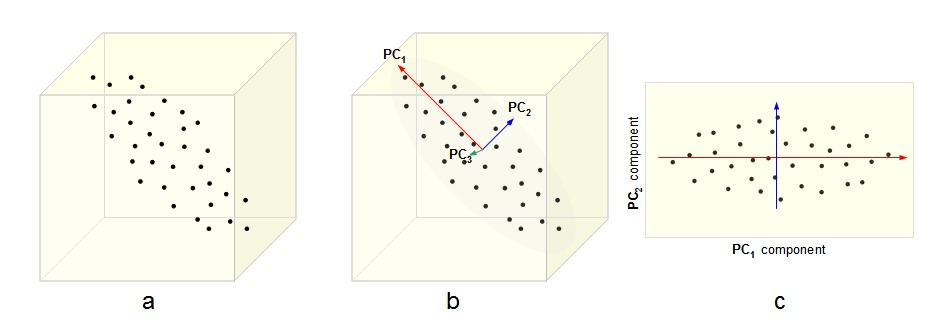
\includegraphics[width=0.8\textwidth]{imgs/pca_1.png}
\caption{ En (a) se muestra un conjunto de datos en tres dimensiones. En (b) se identifican las tres componentes principales (direcciones linealmente decorrelacionadas con mayor variabilidad de datos). En (c) se alinean los datos con las dos direcciones de mayor variabilidad (cambio de base), y se elimina la componente con menor variabilidad. Como consecuencia, la dimensionalidad de los datos se redujo en 1 y pueden ser graficados en el plano. Fuente: \url{cnx.org}  }
\label{fig:pca}
\end{figure}

PCA se calcula en cada paso buscando el versor cuya dirección sea ortogonal a las direcciones de los versores ya calculados, y que maximice la varianza de las proyecciones de los datos sobre dicha dirección. Por construcción, el conjunto de versores generados constituye una base ortonormal.

Luego de calculadas $k$ componentes principales se pueden proyectar los datos sobre dichas direcciones (cambio de base), ignorándose el resto de las componentes. La dimensionalidad se reduce a $k$, capturando -a veces también se dirá ``explicando''- la mayor variabilidad de datos que es posible capturar -o ``explicar''- con cambios de base.\\

También existen métodos de reducción de dimensionalidad que aplican transformaciones no lineales y a veces (dependiendo el conjunto de datos) pueden arrojar mejores resultados. Aún así PCA suele ser suficiente y es adoptado por su sencillez.


\section{Clasificadores}

En la presente sección se describen brevemente algunos clasificadores utilizados en la tesina para encontrar un primer punto de partida (\textit{baseline}) contra el cuál comparar el desarrollo posterior.

\textit{\textbf{Support Vector Machine}} (SVM) es utilizado en \cite{tesis-parodi}, sobre el cuál nuestro trabajo se ha basado fuertemente. También hemos experimentado utilizando \textit{\textbf{Random Forest}} (RF) sobre las características extraídas en el mencionado trabajo.

\textbf{Redes Neuronales Artificiales} (a pesar de ser un clasificador) será desarrollado en la sección siguiente ya que es el método principal utilizado por nuestro trabajo.

\subsection{Random Forest}

\subsubsection{Árboles de Decisión}

Los árboles de decisión son un método simple que consiste en particionar recursivamente mediante hiperplanos el espacio de atributos de modo que quede finalmente partido en hiper-rectángulos \cite{Hastie}. A cada región se le asigna un valor de predicción constante. A la hora de realizar una inferencia sobre un ejemplo $x$ primero se ubicará la región a la que pertenece. Esto puede hacerse siguiendo las reglas de particionado del árbol de decisión binaria que generó las regiones. Finalmente, la predicción será la predicción constante de dicha región. En general el valor constante óptimo para cada región (ajustado sobre el conjunto de datos de entrenamiento) es tomar la media de la variable dependiente $\bar{y}$ en problemas de regresión que usan $MSE$ como métrica, o tomar la etiqueta más frecuente (moda) de las $y_i$ en problemas de clasificación que usan $Error~Rate$ como métrica. Ver figura \ref{fig:randomforest}.

\begin{figure}[h!] 

\centering
\begin{subfigure}{0.33\textwidth}
\centering 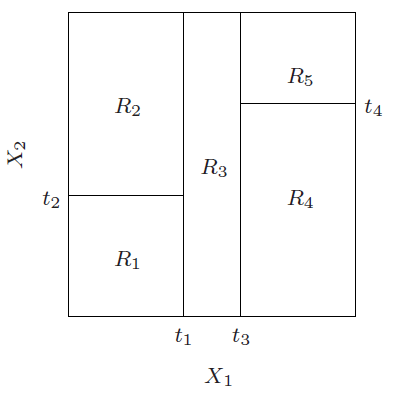
\includegraphics[width=0.3\textwidth]{imgs/decision_tree_1.png}
\end{subfigure}
\begin{subfigure}{0.33\textwidth}
\centering 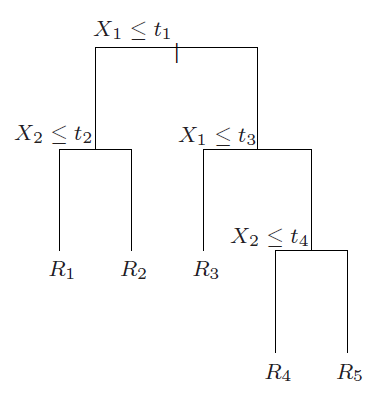
\includegraphics[width=0.3\textwidth]{imgs/decision_tree_2.png}
\end{subfigure}
\begin{subfigure}{0.33\textwidth}
\centering 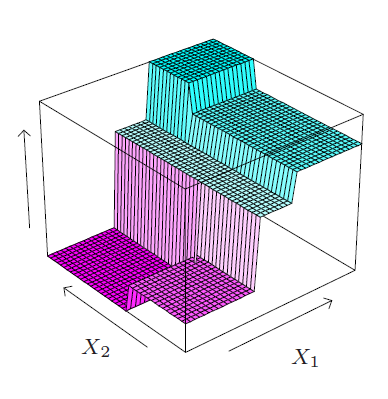
\includegraphics[width=0.3\textwidth]{imgs/decision_tree_3.png}
\end{subfigure}

\caption{ A la izquierda se muestra el espacio de atributos partido en regiones. En el centro se muestra el particionado recursivo (arbol de decisión binaria) que dio como resultado dichas regiones. A la derecha se muestra la función de predicción del modelo que asigna para cada región valores constantes. }
\label{fig:randomforest}
\end{figure}

\subsubsection{\textit{Classification And Regression Tree (CART)}}

El algoritmo de CART es uno de los métodos más populares para construir árboles de decisión. Otras opciones son los métodos ID3 \cite{rf-id3}, C4.5 \cite{rf-c4} y C5.0 \cite{rf-c5}.\\

Para explicar el algoritmo supongamos que tenemos $N$ ejemplos de entrenamiento:
\begin{equation*}
    \{(x_i, y_i), 1 \leq i \leq N\}
\end{equation*}
A su vez consideremos que la variable independiente posee $p$ atributos:
\begin{equation*}
    x_i = ( x_{i,1}, x_{i,2}, ... x_{i,p} ), 1 \leq i \leq N
\end{equation*}

Una partición sobre el atributo $j$ y valor de división $s$ define las regiones $R_1$ y $R_2$ según:
\begin{equation*}
    R_1(j,s) = \{ x | x_{i,j} \leq s, 1 \leq i \leq N \}
\end{equation*}
\begin{equation*}
    R_2(j,s) = \{ x | x_{i,j} > s, 1 \leq i \leq N \}
\end{equation*}
A su vez las predicciones para dichas regiones serán $c_1$ y $c_2$ calculadas como ya se explicó.\\

Para encontrar la mejor partición binaria se optimiza:

\begin{equation*}
    min_{j,s} [ \sum_{x_i \in R_1(j,s)} criterion(y_i, c_1) + \sum_{x_i \in R_2(j,s)} criterion(y_i, c_2) ]
\end{equation*}
Los criterios más usados son $MSE$ para problemas de regresión o \textit{Gini Impurity} o \textit{Information Gain} \cite{rf-inf-gain} para problemas de clasificación.

Para cada uno de los $p$ atributos se puede ordenar en los ejemplos según su $j$-ésima feature con una complejidad de $\mathcal{O}(N~log~N)$  y luego encontrar el mejor valor de división $s$ con una complejidad $\mathcal{O}(N)$. Haciendo esto para cada atributo $j$ se puede encontrar la mejor elección de $s$ sumando una complejidad total de: $\mathcal{O}(p N~log~N)$) en cada paso de subdivisión nueva del árbol. Incluso se puede ordenar una vez al principio y mantener $p$ listas (una para cada atributo) de índices que apunten a los $x_i$ ordenada según dicho $j$-ésimo atributo, ahorrando el factor $log N$ en cada paso.

El algoritmo CART encuentra la mejor partición binaria, se particionan los datos en las regiones resultantes y se repite recursivamente el proceso de división. La decisión de partir en la mejor partición en cada paso es una decisión \textit{greedy}. Optimiza la mejor decisión local, o sea en un único paso de subdivisión, aunque puede no ser la mejor decisión global, o dicho de manera más coloquial ``al largo plazo''. De todas formas llega a muy buenos resultados de árboles de decisión. \\

\textbf{Ventajas de los Árboles de Decisión:} 
\begin{itemize}
    \item Poseen bajo sesgo, pués no hacen demasiadas asumpciones en la función objetivo.
    \item Son simples, no poseen demasiados hiperparámetros a ajustar.
    \item Son robustos al escalado de los atributos. No requieren normalizar o estandarizar los datos. Son insensibles a estos preprocesamientos puesto que sólo importa el orden de los características, no su escala.
\end{itemize}

\textbf{Desventajas de los Árboles de Decisión:}
\begin{itemize}
    \item Los árboles profundos poseen alta varianza, por lo cuál, de no configurar bien los hiperparámetros que controlan su complejidad (cantidad mínima de nodos, profundidad máxima o aplicar técncias de podas) son propensos a sobreajustar.
    \item Al predecir valores constante para cada región son incapaces de descubrir tendencias que permitan extrapolar las predicciones a rangos de atributos que no estén dentro del rango de los atributos presente en el conjunto de entrenamiento; potencialmente arrojando resultados erróneos para ellos. Ver figura \ref{fig:rf-extrapolation-problem}.
    
    A diferencia de lo que muchos creen, no es un problema que tengan sólo en problemas de regresión sino que se pueden pensar casos en donde afecten a problemas de clasificación (por ejemplo distinguir la clase de los $(x_1,x_2)$ donde $|x_1 - x_2 | \leq 1$). Y es que la escencia del problema radica en que las regiones con valores constantes no predicen bien ejemplos que poseean atributos ``más allá'' de los rangos de los atributos presentes en el entrenamiento.
\end{itemize}

\subsubsection{\textit{Random Forest}}

Para mitigar el problema de la alta varianza de los árboles de decisión se puede recurrir a \textit{\textbf{decision tree bagging}}. En este método se entrena un número $t$ de árboles de decisión, cada uno basado en diferentes subconjuntos de $m$ ejemplos tomados del conjunto de datos de entrenamiento y luego (para la inferencia) se combinanan los resultados de las predicciones, por ejemplo, tomando la media o moda. Cuándo se combinan modelos se suele hablar de \textit{\textbf{ensamble}}.

Esta técnica es denominada \textit{\textbf{Bagging}} y puede aplicarse sobre cualquier predictor \cite{breiman-1993}. Es un caso particular de la técnica denominada \textit{\textbf{Bootstrap}}, utilizada para encontrar buenos estimadores estadísticos sobre una población \cite{Hastie}. Tiene la capacidad de reducir dramáticamente la varianza de predictores inestables como árboles de decisión sin introducir sesgo, lo cual conduce a mejores resultados. Una propiedad importante de los \textit{ensambles} es que al incrementar el número $t$ de estimadores base utilizados, el valor de la predicción no puede empeorar. Como  contrapartida, la construcción será más lenta (un factor lineal respecto de $t$). \\

\textit{\textbf{Random Forest}} es una modificación de un \textit{\textbf{decision tree bagging}} donde además de la técnica de \textit{bagging} se agrega que, cuando se crean los árboles de decisión, en cada nivel a subdividir se consideran aleatoriamente sólo $k$ de los $p$ atributos como candidatos. Ésto introduce ruido en el proceso que ayuda a que los $t$ árboles generados no estén tan correlacionados, reduciendo aún más la varianza del \textit{ensamble}. \cite{breiman-2001}. 
Valores pequeños de $k$ reducirán la correlación entre cada par de árboles del ensamble, y por lo tanto, reducirán la varianza en promedio. Generalmente se toma $k = \sqrt{p}$. \\

\textbf{OOB (\textit{out of bag}):} para cada ejemplo $x_i$ del conjunto de datos, es posible construir una predición de \textit{Random Forest} promediando sólo las predicciones de aquellos árboles que no incluyeron a $x_i$ en el conjunto de entrenamiento. Esto es lo que se conoce como \textit{\textbf{OOB score}}. El \textit{OOB score} constituye una métricas de validación correcta y es calculada haciendo uso de elementos incluídos en el conjunto de entrenamiento, lo que implica que no necesitamos reservar datos para la validación. ¡Podemos entranar con todos los datos!.

Es importante notar que si el \textit{Random Forest} posee $t$ predictores, durante el cálculo del \textit{OOB score} se utiliza para cada ejemplo una cantidad menor de predictores (ya que se obvian para cada ejemplo los que lo utilizaron para entrenar). Es por ello que el \textit{OOB score} será una métrica \textit{pesimista} (se pueden esperar mejores resultados sobre un conjunto de test). También es importante aclarar que al igual que el método de \textit{Cross-Validation}, \textit{OOB Score} se basa en la asumpción de que un particionado aleatorio del conjunto de datos constituye una buen conjunto de validación. De no ser cierto esto observaremos un considerablemente mejor \textit{OOB score} que los resultados observados sobre un conjunto de test bien confeccionado.\\

\textbf{Ventajas de \textit{Random Forest}:} tienen la simplicidad de los árboles de decisión (pocos hiperparámetros, insensible a la escala de atributos) y respecto a los mismos, resuelve el problema de sobreajuste causado por la alta varianza.\\

\textbf{Desventaja de \textit{Random Forest}:} no solucionan el problema de extrapolación que poseen los árboles de decisión. Ver figura \ref{fig:rf-extrapolation-problem}.

\begin{figure}[h]
\centering
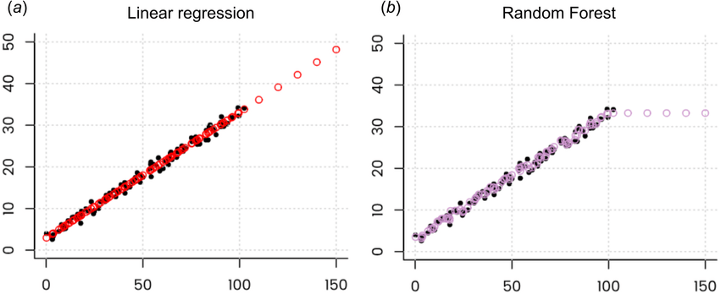
\includegraphics[width=0.9\textwidth]{imgs/rf_extrapolation_problem.png}
\caption{Ejemplo del problema de extrapolación que poseen los árboles de decisión y hereda el método de Random Forest. Créditos: Derrick Mwiti \url{https://neptune.ai/blog/random-forest-regression-when-does-it-fail-and-why} }
\label{fig:rf-extrapolation-problem}
\end{figure}






\subsection{Support Vector Machine}

Las Máquinas de Vectores Soporte son un método de clasificación que está sustentada por un desarrollo matemático teórico de envergadura ya que se basa en aprendizaje estadístico o teoría VC (Vapnik-Chervonenkis) \cite{svm-vapnik1}, \cite{svm-vapnik2}.\\

Procederemos a explicar intuitivamente y de manera sencilla las ideas claves. Atiunque haremos referencias a las formulaciones matemáticas, no profundizaremos en ellas. El lector puede ampliar sobre el desarrollo del método leyendo \cite{svm-genesis1} \cite{svm-genesis2} o ahondar en el desarrollo matemático en \cite{Hastie}.

\begin{enumerate}
    \item Una tarea de clasificacióin puede ser vista como la tarea de separar los espacios geométricos que ocupa cada clase dentro del espacio de atributos. Ver figura \ref{fig:svm-seperadores}.
    
\begin{figure}[h!]
\centering
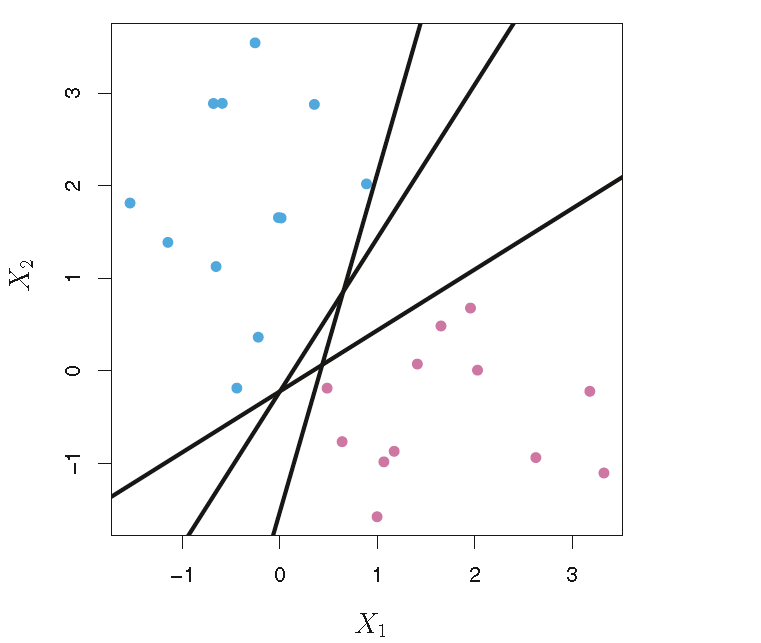
\includegraphics[width=0.45\textwidth]{imgs/svm_separadores.png}
\caption{ Ejemplo de clasificación binaria particionando el espacio geométrico de atributos por medio de separadores lineales.  Créditos: Drew Wilimitis, \url{towardsdatascience.com} }
\label{fig:svm-seperadores}
\end{figure}

    \item Podemos empezar tratando de utilizar hiperplanos de la forma $wx+b=0$ para separar las clases. De todos los hiperplanos a elegir en nuestra labor de optimización encontraremos el que maximice el margen entre ambas clases: la mínima distancia entre un punto del conjunto de entrenamiento y el hiperplano separador. Ver figura \ref{fig:svm-hiperplanos}.
    
\begin{figure}[h!]
\centering
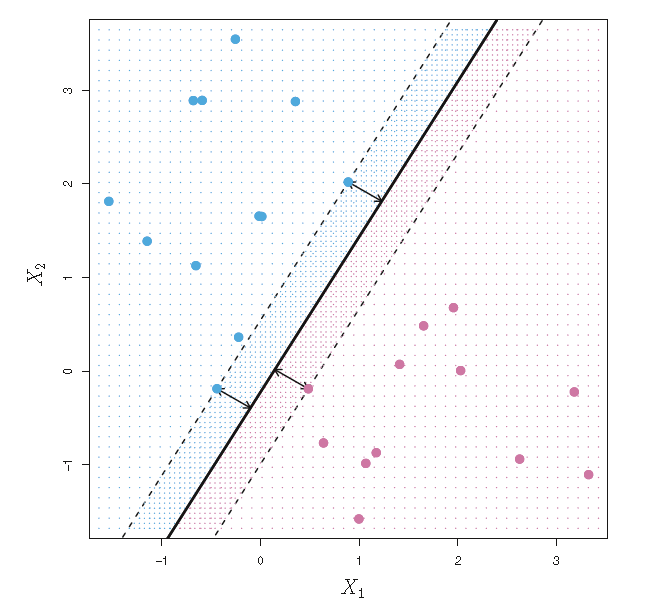
\includegraphics[width=0.45\textwidth]{imgs/svm_hiperplanos.png}
\caption{ Ejemplo de hiperplano calculado por SVM. Los puntos que están a menor distancia del hiperplano separador se denominan vectores soporte. Créditos: Drew Wilimitis, \url{towardsdatascience.com} }
\label{fig:svm-hiperplanos}
\end{figure}
    
    \item La contra es que puede no existir un hiperplano que los separe, por ejemplo, si las clases se encuentran ``demasiado superpuestas'' en el especio de atributos. Ver figura \ref{fig:svm-imposible}.
    
\begin{figure}[h!]
\centering
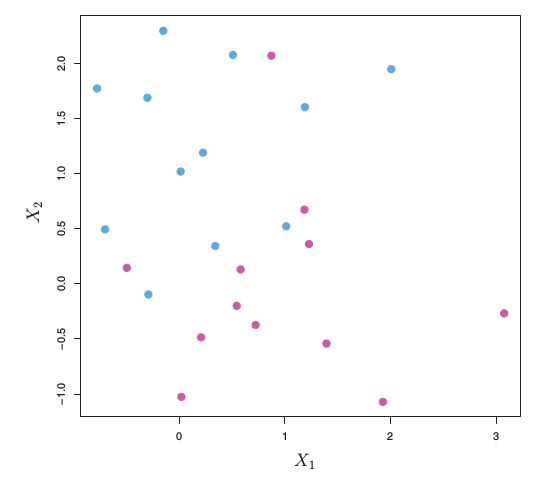
\includegraphics[width=0.45\textwidth]{imgs/svm_imposible.png}
\caption{ En este ejemplo de clases celestes y violetas, no pueden ser separadas por un hiperplano. Créditos: Drew Wilimitis, \url{towardsdatascience.com} }
\label{fig:svm-imposible}
\end{figure}
    
    \item Podemos debilitar el problema de separar las clases utilizando márgenes ``relajados'' y permitiendo a algunos puntos de entrenamiento estar dentro del lado equivocado del hiperplano. Ver figura \ref{fig:svm-margenes}.

\begin{figure}[h!]
\centering
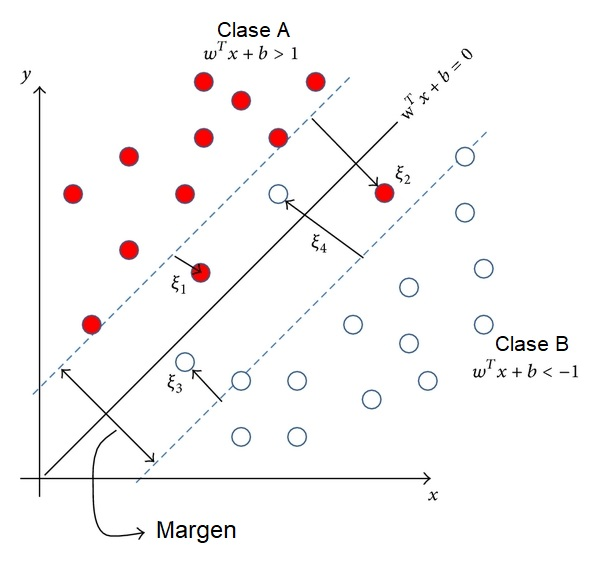
\includegraphics[width=0.6\textwidth]{imgs/svm_margenes.png}
\caption{ Los valores notados como $\epsilon_i$ constituyen una medida de margen relajado para cada ejemplo y se denominan \textit{variables slack}.
El hiperparámetro C permite regular cuán permisivo es el modelo a la hora de permitir errores de clasificación. Imagen tomada de \cite{svm-margenes}. }
\label{fig:svm-margenes}
\end{figure}    

    En la formulación matemática minimizaremos no sólo la distancia mínima al hiperplano separador sino también un término que pondere \textit{``que tanto nos permitimos relajar los márgenes''}. De aquí sale el hiperparámetro $C$ llamado \textit{coste} o \textit{regularización}.
    
    \item Seguimos teniendo el limitante de que las fronteras son sólo lineales: puede no ser lo ideal para muchas distribuciones de datos. Es por eso que se introduce una función $\phi$ que mapee los datos de la variable independiente $x$ a un espacio de mayor dimensionalidad donde potencialmente las clases serán separables por una frontera lineal. Así, trataremos de usar la formulación de hiperplano ya desarrollada hasta el punto anterior no para los datos $\{(x_i, y_i)\}$ sino para separar $\{(\phi(x_i), y_i)\}$. Ver figura \ref{fig:svm-kernel}.
    
\begin{figure}[h!]
\centering
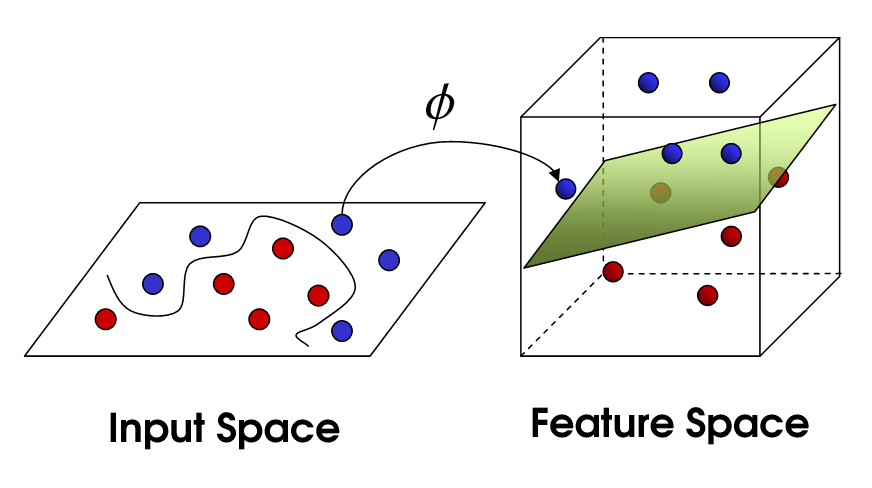
\includegraphics[width=0.6\textwidth]{imgs/svm_kernel.png}
\caption{ Luego de mapear los puntos por medio de una función no lineal a un espacio de mayor dimensionalidad pueden ser separados por un hiperplano. Remitiéndonos al espacio de atributos original el hiperplano constituye una superficie curva que particiona el espacio. Créditos: Drew Wilimitis, \url{towardsdatascience.com}  }
\label{fig:svm-kernel}
\end{figure}    
    
    \item El punto anterior no tiene sentido sin lo que se denomina \textbf{truco de kernel}: trabajando algebraicamente la fórmula a optimizar se llega a una expresión tal que nunca es necesario para la optimización calcular explícitamente el mapeo $\phi(x)$ sobre los ejemplos, sólo es necesario saber como calcular productos internos sobre el resultado de dichos mapeos (en el espacio de mayor dimensionalidad).
    
    O sea simplemente necesitamos saber como calcular:
    \begin{equation*}
        K(x_i, x_j) = <\phi(x_i), \phi(x_j)>
    \end{equation*}
    Donde $<,>$ es la operación de producto interno. Dicha función $K$ se denomina \textbf{función kernel}. Se desarrollan varias de estas funciones en la bilbiografía citada  que poseen un sustento teórico relevante. Su elección y la de sus parámetros constituyen hiperparámetros de las SVM.

\end{enumerate}



\section{Redes Neuronales Artificiales}

Las \textbf{Redes Neuronales Artificiales} (\textit{RNA} por sus siglas en inglés) son un método de aprendizaje supervisado que deben su nombre a su raíz histórica: surgen a partir de diferentes trabajos que trataron de imitar el funcionamiento del cerebro humano. Sin embargo, la investigación moderna está guiada por disciplinas matemáticas y de ingeniería, y el objetivo de las RNA no es modelar perfectamente el cerebro.

\subsection{Un poco de historia}\label{subsection:intro-redes}

En 1943 el lógico Walter Pitts propone un modelo simplificado de la neurona cerebral representado por adiciones y la aplicación de un umbral. Intentaba imitar y analizar el comportamiento del cerebro humano en su trabajo \textit{``A Logical Calculus of the Ideas Immanent in Nervous Activity''} \cite{pitts}. Él creía que la neurona se podía modelar como adición de sus entradas y aplicación de una función de umbral para producir las respuestas debido a que la actividad neuronal poseía lo que describía como \textit{``caracter de activación de todo o nada''} (ver figura \ref{fig:pitts}).

\begin{figure}[h!]
\centering
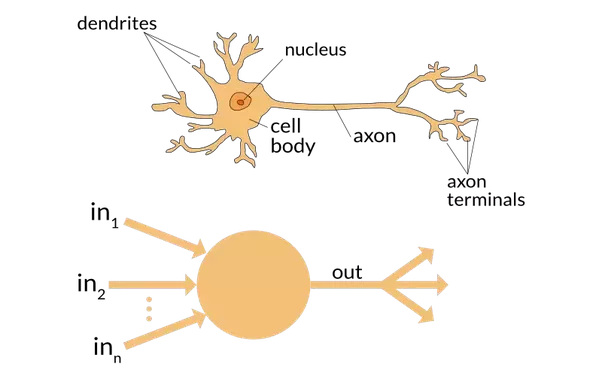
\includegraphics[width=0.6\textwidth]{imgs/walter_pitts.png}
\caption{ Imágen esquemática del modelo de neurona propuesto por \cite{pitts}. Fuente: \cite{fastbook}. }
\label{fig:pitts}
\end{figure}

En 1958 el psicólogo Frank Rosenblatt desarrolla la neurona artificial (Mark I Perceptrón) con habilidad para aprender en \textit{``The Design of an Intelligent Automaton''} \cite{rosenblatt}. El mismo poseía la siguiente formulación (ver figura \ref{fig:perceptron}) \cite{perceptron}:

\begin{equation*}
    o(x_1, ..., x_n) = \left\lbrace\begin{array}{l} ~~1~si~w_0 + w_1 x_1 + w_2 x_2 + ... + w_n x_n > 0 \\ -1~en~caso~contrario \end{array}\right.
\end{equation*}

Los parámetros $w_i$ se inicializarían de manera aleatoria y actualizarían iterativamente comparando la salida $o$ del perceptrón con la salida esperadas $y$, siguiendo la siguiente fórmula: 
\begin{equation*}
    w_i \leftarrow w_i + \Delta w_i
\end{equation*}
\begin{equation*}
    \Delta w_i = \eta (y - o) x_i
\end{equation*}
Donde $x_i$ es el atributo respectivo al peso que se está actualizando y $\eta$ una constante que denominada \textit{learning rate}. En \cite{allen-newell} se ha demostrado que de ser $\eta$ suficientemente pequeña, en un problema binario linealmente separable el algoritmo converge a la solución óptima. El procedimiento es análogo al método de descenso por gradiente que se verá en las próximas secciones y en el cuál se basa la optimización de las actuales redes neuronales.

\begin{figure}[h!]
\centering
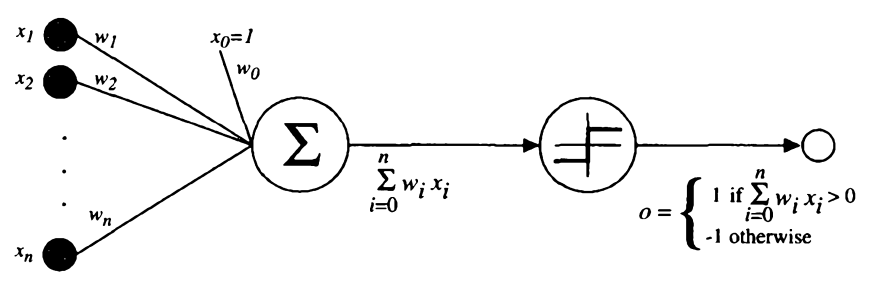
\includegraphics[width=0.6\textwidth]{imgs/perceptron.png}
\caption{ Representación gráfica de un perceptrón. Fuente \cite{perceptron}.  }
\label{fig:perceptron}
\end{figure}

El preceptrón de Rosenbalt cayó en el olvido luego de que una publicación del profesor de MIT (colega de Rosenbaltt) Marvin Minsky demostrara que no podía representar simples funciones como XOR. Este perceptrón puede verse como un hiperplano partiendo el espacio de atributos de manera que produce una salida igual a 1 para instancias que se encuentran a un lado del hiperplano, y -1 al otro. Por eso la efectividad está limitada a conjuntos de datos linealmente separables. \\


Otro antecedente histórico de imitar la estructura de comportamiento del cerebro se haya en \textit{``Parallel Distributed Processing (PDP)''} \cite{PDP} donde se describe que de existir un sistema tal, poseería las siguientes características (todas características que poseen las redes neuronales actualmente):
\begin{enumerate}
    \item Un conjunto de unidades de procesamiento.
    \item Un estado de activación de las mismas.
    \item Una función de salida de cada unidad de procesamiento.
    \item Un patrón de conectividad de dichas unidades.
    \item Una regla de propagación de las activaciones a través de la red de conexiones (forma de transformar las salidas de una unidad en entradas de la otra).
    \item  Una regla de activación para combinar las entradas de las unidades, el estado actual y producir las salidas de la unidad.
    \item Una regla de aprendizaje donde se modifican los patrones de conectividad por medio de la experiencia.
    \item Un entorno en donde el sistema opera.
\end{enumerate}

Durante la década del 80' las redes neuronales vuelven a cobrar cierta tracción en el mundo científico a raíz de que se demostrara que agregar una segunda capa de neuronas evitaría el problema identificado por Minsky \cite{universal-width}. Véase figura \ref{fig:one-layer} \\

\begin{figure}[h!]
\centering
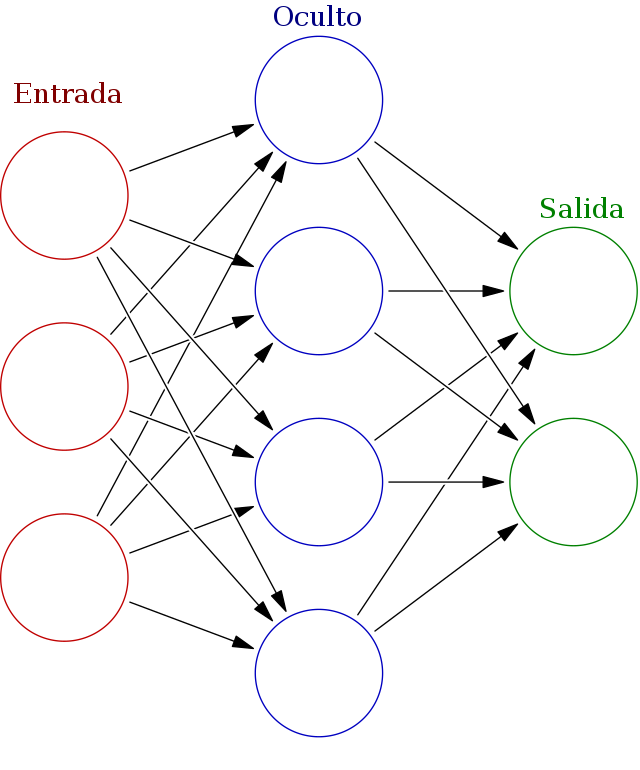
\includegraphics[width=0.4\textwidth]{imgs/one_layer.png}
\caption{ Esquema de red de una capa oculta. Las entradas se combinan linealmente y se le aplica una función no lineal para obtener las activaciones ocultas (valores intermedios) que luego se vuelven a combinar linealmene y aplicar una función no lineal para obtener las salidas o predicciones.  
Créditos de la imágen: \url{es.wikipedia.org/wiki/Red_neuronal_artificial} }
\label{fig:one-layer}
\end{figure}

En 1986 se publicaron los reconocidos trabajos sobre el método de \textit{backpropagation} donde se establece el algoritmo de optimización que hasta el día de hoy es utilizado (con algunas variaciones y ajustes) para entrenar las redes neuronales de muchas capas \cite{backpropagation1} y \cite{backpropagation2}. No obstante actualmente se sabe que esta técnica fue varias veces re-descubierta e incluso existe un antecedente que data de 1960 \cite{backpropagation3}.\\

Si bien teóricamente cualquier función continua puede ser aproximada por redes con una capa oculta con un número suficiente de neuronas se falló en entender la naturaleza fundamentalmente empírica del aprendizaje automatizado y poco se exploró aproximadamente hasta 20 años después sobre el potencial de agregar más capas. 
A fines de los 90' se publica el famoso trabajo \cite{lenet} que mejora sustancialmente la performance utilizando un modelo relativamente sencillo (LeNet-1) y sin extracción manual de caraceterísticas. Fue este el nacimiento de las redes convolucionales que revolucionaron el mundo de la visión computarizada.

\subsection{Formulación actual} \label{subsection:nn-formulacion}

La formulación actual de las Redes Neuronales Artificiales no dista demasiado del modelo simplista de red de una capa oculta, descripto en la subsección anteior. Ver figura \ref{fig:one-layer}. 

Supongamos que la función a aproximar es: 
\begin{equation*}
\hat{f} : \mathbb{R}^{n_{in}} \rightarrow \mathbb{R}^{n_{out}}
\end{equation*}
O sea que tenemos $n_{in}$ atributos de entrada y $n_{out}$ de salida.


Una Red Neuronal Artificial consiste escencialmente en transformar el vector de entradas $\{x_i\}_{i=1}^{n_{in}}$ aplicando sucesivamente funciones no lineales $f^j$ denominadas \textbf{capas}. Estas funciones tienen la forma:
\begin{equation*}
    f^j : \mathbb{R}^{w_{j-1}} \rightarrow \mathbb{R}^{w_j}
\end{equation*}

O sea, son simples transformaciones de vectores en vectores. Notaremos $\bar{h}^j = \{h_i^j\}_{i=1}^{w_j}$ el resultado de la $j$-ésima capa. Los resultados de cada capa son denominados \textbf{activaciones} \cite{libro-nielsen}. 

Definiendo $\bar{h}^0 = x$ que constituye la entrada de nuestra red y a menudo se la llama \textbf{capa de entrada}. 

A la dimensión de la capa $\bar{h}^j$, notada $w_j$ se la conoce como \textbf{anchura de la capa}.


Cada una de dichas funciones (capas, de ahora en más) consiste en una transformación afín de la salida de la capa anterior (o el vector de entrada para el caso de la primer capa), seguida de una función no lineal $\phi^j$ (denominada \textbf{función de activación}). 


Los modelos donde la información fluye desde la entrada hasta la salida sin retroalimentaciones se denominan \textit{\textbf{feed forward}} (ver figura \ref{fig:feedforward}). 

Suponiendo que tenemos $m$ capas, el vector de las $\{h_i^m\}_{i=1}^{n_{out}}$ constituyen la salida de nuestra red. El número $m$ de capas se denomina \textbf{profundidad}.

Podemos formular una red neuronal \textit{feed forward} más formalmente -y de forma concisa- como:

\begin{equation*}
    \bar{h^0} = \bar{x}
\end{equation*}
\begin{equation*}
    \bar{h}^{j+1} = f^{j+1}(\bar{h}^j)
\end{equation*}
\begin{equation*}
    out_i = h_i^m ~ 0 \leq i < n_{out}
\end{equation*}
Donde:
\begin{equation*}
    f^j(\bar{h}^{j-1}) = \phi^j( {W^j}^\top \bar{h}^{j-1} + b^j)
\end{equation*}

\begin{figure}[h!]
\centering
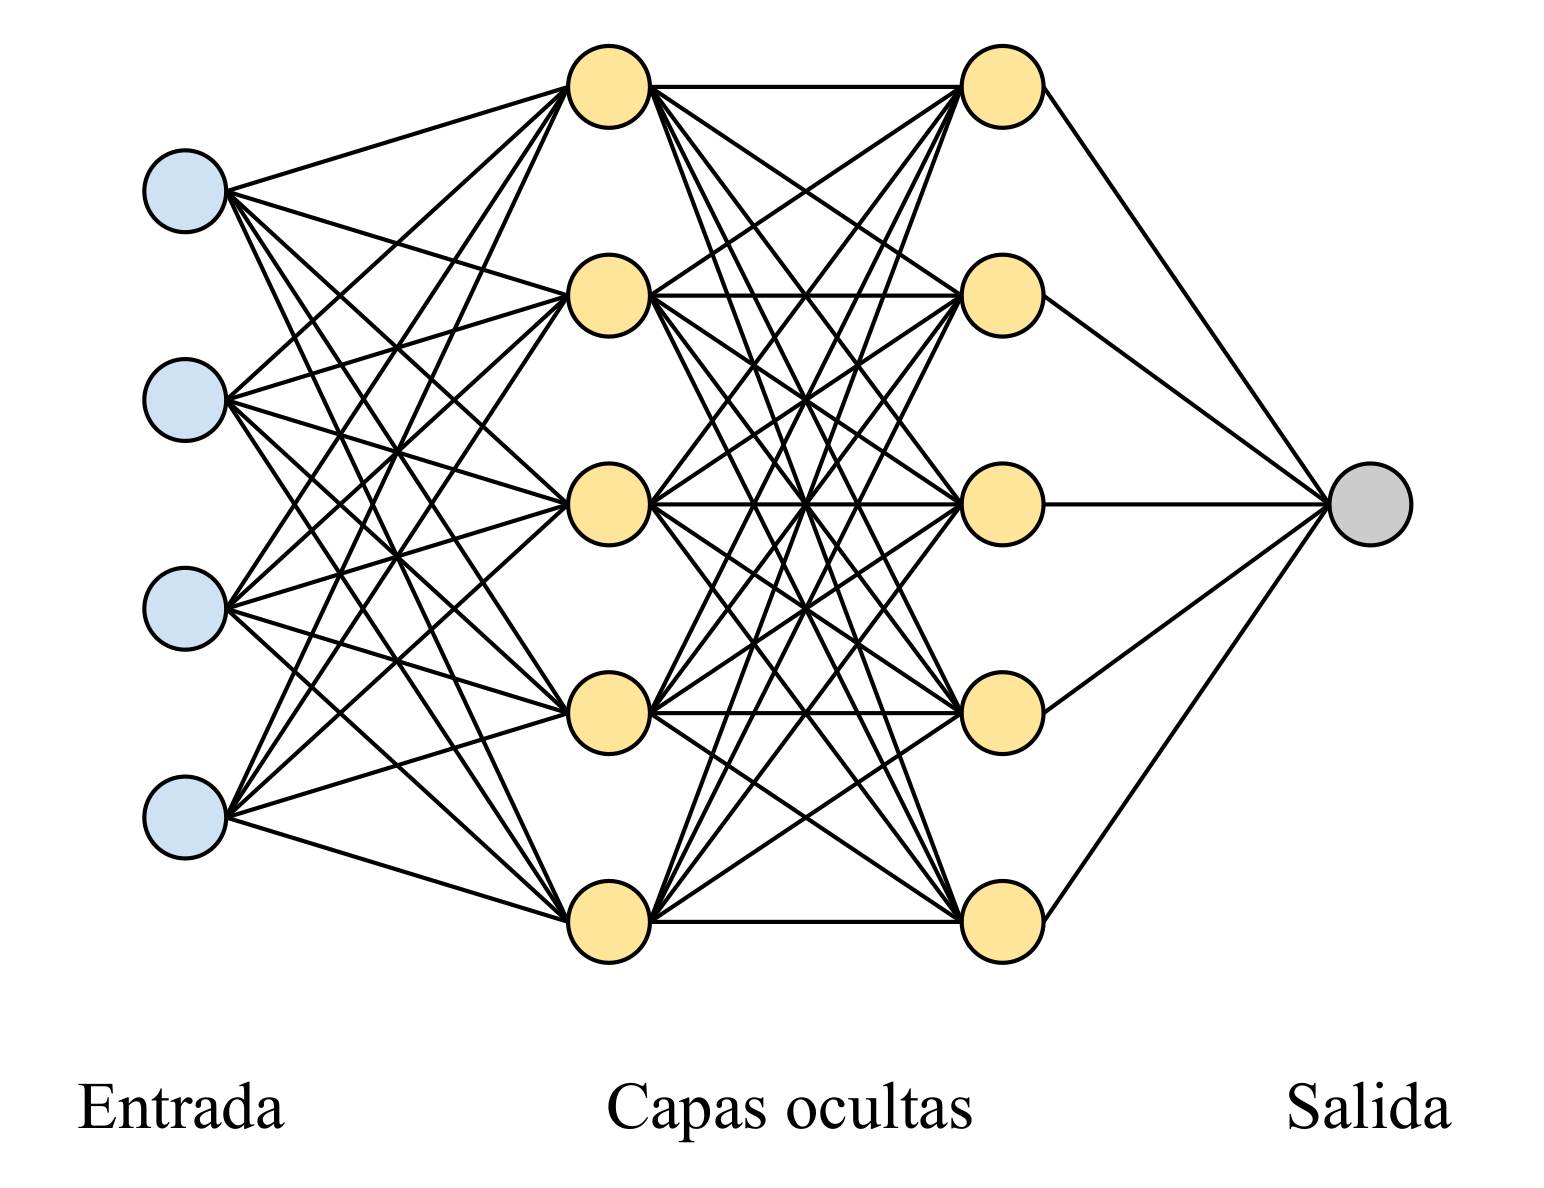
\includegraphics[width=0.4\textwidth]{imgs/feedforward.png}
\caption{ Esquema de un modelo de red neuronal \textit{feed forward}. Análogamente a los modelos de una única capa oculta, las entradas se combinan linealmente y se le aplica una función no lineal para obtener activaciones ocultas. Existe un vector de activaciones ocultas por cada capa de valores intermedios (capa oculta) que resulta de combinar linealmente y aplicar una función no lineal sobre la capa anterior. Finalmente la última capa constituye la salida del modelo. Imágen extraída de \cite{tesina-marcos} }
\label{fig:feedforward}
\end{figure}

Los valores de las matrices $W^j \in \mathbb{R}^{w_{j-1} \times w_j}$, $b^j \in \mathbb{R}^{w_j}$ son los parámetros a entrenar y se denominan respectivamente \textbf{pesos} y \textit{\textbf{biases}} en la jerga del aprendizaje profundo. Son responsables del cambio de dimensión de una capa a otra de activaciones aplicando una transformación afín. La función de activación $\phi^j$ generalmente es una simple función $\mathbb{R} \rightarrow \mathbb{R}$ que es aplicada de forma independiente componente a componente. 

Fijado el número $m$ de capas, sus respectivas anchuras $w_j$ y funciones de activación $\phi^j$ queda definida ``el esquema'' de la red: la cantidad de parámetros y su relación con las entradas queda fija. Las salidas solo dependerán de la elección de los parámetros. Ésto es lo que se conoce como \textbf{arquitectura} del modelo o red.\\

\sout{\textbf{Nota:} El Aprendizaje Profundo posee una jerga entrevesada para conceptos realmente simples. A menudo ésto ocurre a raíz de llamar de manera \textit{vistosa} ciertos conceptos que ya existían para que suenen más innovadores a lo largo de las publicaciones que los han popularizado. Hay que evitar que esta jerga científica nos haga perder de vista la simpleza de los conceptos subyacentes del Aprendizaje Profundo: \textbf{función de activación} no es más que una función no lineal, \textbf{activaciones} son resultados parciales. En las secciones subsiguientes se seguirán introduciendo conceptos con nombres estrambóticos que tienen significados muy simples como las \textbf{unidades rectificadoras} que son simplemente la función $max(0,x)$. ¡Los principios matemáticos detrás de las Redes Neuronales Artificiales son realmente simples! \\}

\textbf{Observación:} Con los conceptos definidos tenemos un panorma de Red Neuronal Artificial que satisface casi todos los puntos que en \textit{``Parallel Distributed Processing (PDP)''} \cite{PDP} se planteaba como necesario para \textit{``imitar al cerebro humano''}. Tan sólo nos falta tener una forma de evaluar la experiencia y una regla de aprendizaje, que es lo que veremos en las secciones siguientes.

\subsection{Descenso por gradiente} \label{subsection:descenso-gradiente}

En esta sección describiremos la \textbf{regla de aprendizaje} utilizada para \textit{ajustar} el modelo. Definida la arquitectura de una red neuronal, resta elegir valores óptimos de los parámetros $W^j$, $b^j$. Por simplicidad notaremos para esta sección al conjunto de todos los parámetros (\textit{pesos} y \textit{biases}) con $W$. Primero que nada necesitamos definir precisamente qué queremos optimizar. Supongamos que poseemos una función $J$ para medir el error de nuestro modelo al aproximar la función objetivo dada una determinada asignación de pesos: 
\begin{equation*}
    J :  \mathbb{R}^{|W|} \rightarrow \mathbb{R}_0^+
\end{equation*}

Por ahora podemos pensar que $J$ calculará las predicciones (salidas de la red) para cada ejemplo del conjunto de datos y lo comparará \textit{de alguna forma} con las salidas esperadas. \\

\textbf{Nota}: notar que $J$ recibe como entrada los \textit{parámetros} del modelo. El conjunto de datos de evaluación (que será provisto como entrada al modelo) se considera fijo para el análisis de $J$. El conjunto de datos no es una entrada de la función $J$.\\

Las funciones que se utilizan para medir el error, comparando las entradas y las salidas son llamadas \textbf{funciones de costo}. En la sección siguiente se habla de qué funciones de costo se usan para cada problema y qué diferencia tiene con el concepto ya definido de \textit{métricas}. 

El método de actualización se basa en el gradiente\footnote{Recordar que el concepto de \textit{gradiente} para una función $\mathbb{R}^n \rightarrow \mathbb{R}$ es un vector donde cada componente es la derivada de la -única- salida respecto de cada componente de la entrada. \cite{apostol} \cite{math-ml} } de los pesos en función del costo:

\begin{equation*}
    \nabla J(W) = \left ( \frac{\delta J}{\delta W_0}, \frac{\delta J}{\delta W_1} , ... , \frac{\delta J}{\delta W_m}  \right )
\end{equation*}

Gráficamente puede interpretarse al gradiente como la dirección (en el espacio de pesos) donde ocurre el mayor incremento de $J$ de manera local (dentro de un entorno infinitamente pequeño). De manera opuesta $- \nabla J(W)$ determina la dirección de mayor decremento local.

El algoritmo de descenso por gradiente usa esto y actualiza los pesos ``moviéndose'' en la dirección opuesta al gradiente (ver figura \ref{fig:gradiente}):

\begin{equation*}
    W_i \leftarrow W_i - \eta \nabla J_i(W)
\end{equation*}

$\eta$ es una constante positiva llamada \textit{\textbf{learning rate}} que determina cuánto se modifica $W$ en la dirección y magnitud del gradiente del costo. Notar que ésta fórmula es similar a la de actualización del original Perceptrón \cite{perceptron}. \

\begin{figure}[h!]
\centering
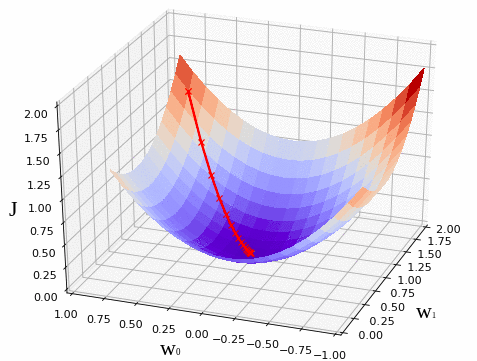
\includegraphics[width=0.6\textwidth]{imgs/descensogradiente.png}
\caption{ Ejemplo de descenso por gradiente en un espacio de dos parámetros para una función de costo convexa. En la práctica los espacios de pesos son de altísima dimensionalidad y las funciones suelen no ser suaves y poseer mínimos locales y puntos de ensilladura. Imágen extraída de \cite{tesina-marcos}  }
\label{fig:gradiente}
\end{figure}

El algoritmo converge cuando se alcanza un punto crítico (gradiente cero). Notar que en casos donde la función no es convexa es posible que el algoritmo converja a \textbf{mínimos locales} (que no sean el mínimo global) o \textbf{puntos de ensilladura} (ver figura \ref{fig:localmin}).

\begin{figure}[h!]
\centering
\begin{subfigure}{0.45\textwidth}
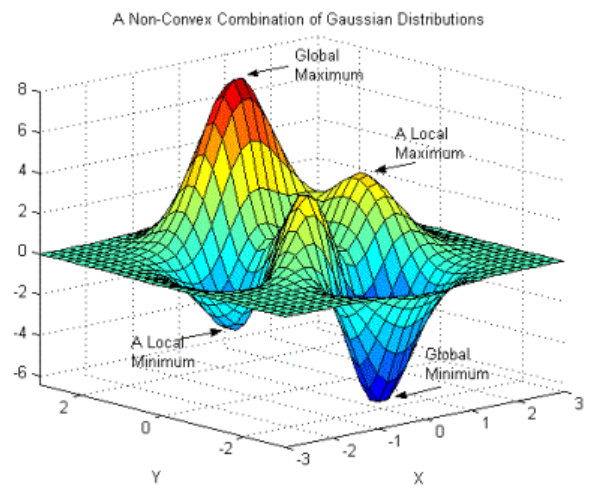
\includegraphics[width=0.4\textwidth]{imgs/localmin.png}
\end{subfigure}
\begin{subfigure}{0.45\textwidth}
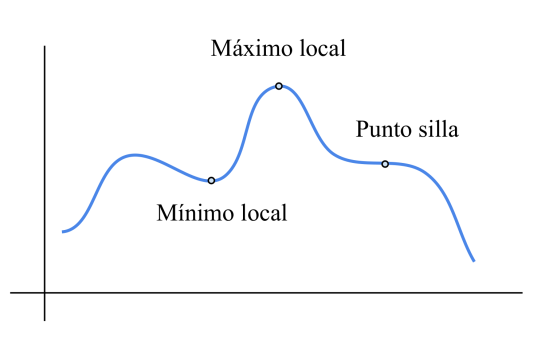
\includegraphics[width=0.4\textwidth]{imgs/critico.png}
\end{subfigure}

\caption{ En la figura izquierda podemos ver un ejemplo de función de dos parámetros no convexa. Se señalaron los mínimos locales. En la figura derecha se muestran los dos tipos de puntos críticos: mínimos y máximos locales, y puntos de ensilladura. El máximo global es un caso particular de éstos. Imágen extraída de \cite{tesina-marcos} y \cite{tesina-zanetti}. }
\label{fig:localmin}
\end{figure}

En la práctica las funciones de costo poseen formas irregulares como muestra el trabajo \cite{visualizing-landscapes}, con varios mínimos locales (ver figura \ref{fig:loss_surface}). Pero se ha corroborado que no encontrar mínimos globales no constituye un problema siempre que se encuentren mínimos locales con bajo costo \cite{deeper-better}. Además \cite{no-chair} muestra que para muchas funciones no convexas de alta dimensionalidad, los mínimos locales son infrecuentes respecto a los puntos ensilladura.

\begin{figure}[h!]
\centering 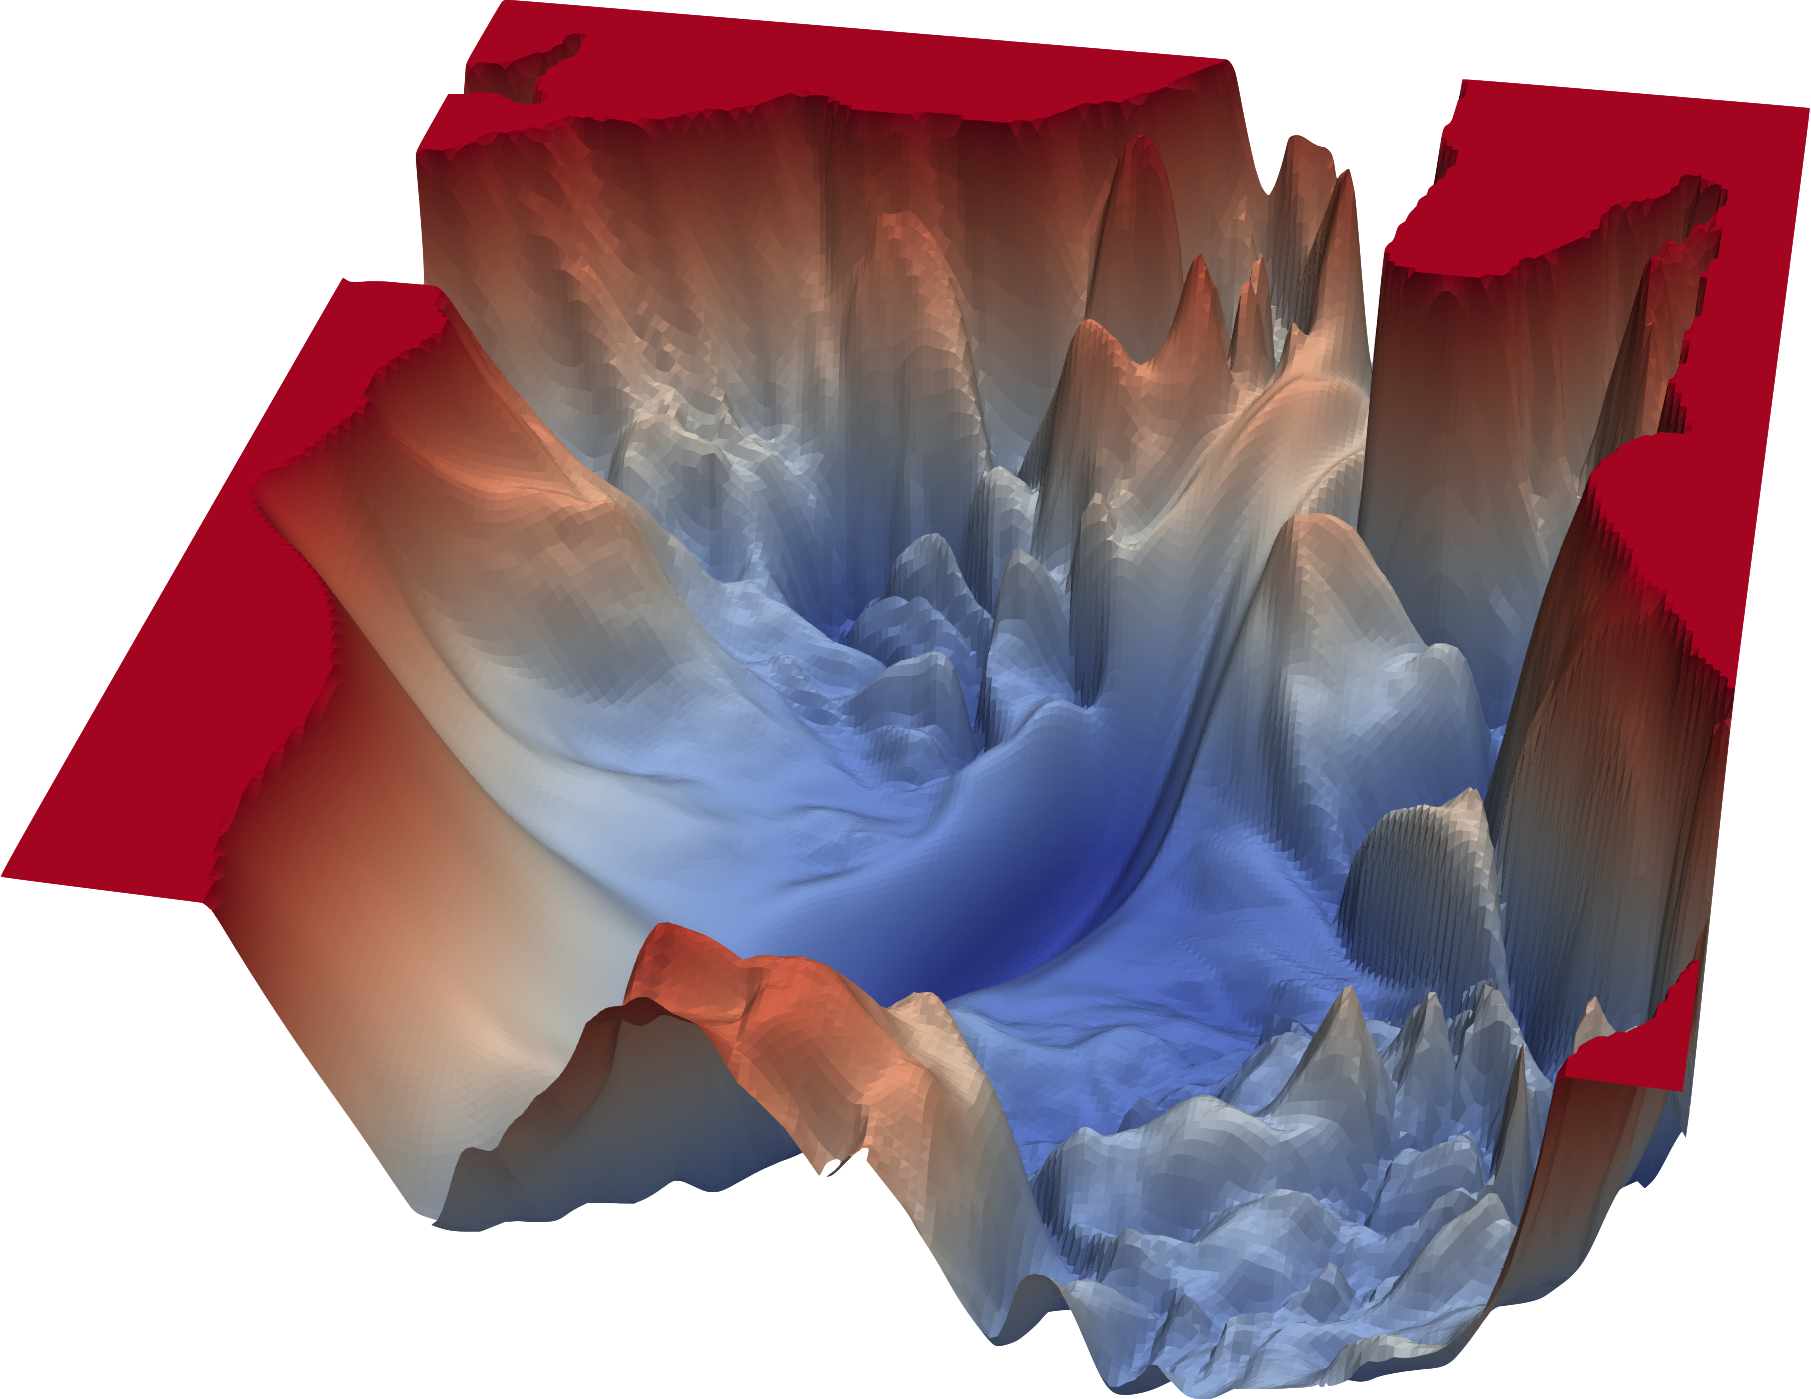
\includegraphics[width=0.4\textwidth]{imgs/loss_surface.png}

\caption{ Visualización en dos dimensiones de la función de costo sobre un conjunto de datos reales. Fuente: \cite{visualizing-landscapes}. }
\label{fig:loss_surface}
\end{figure}

\subsubsection{Sobre funciones de costo ``\textit{realistas}''} \label{subsubsection:sharped-mins}

Las funciones de costo dependen tanto de la arquitectura como del conjunto de datos. Esta característica conceptual tiene una implicancia metodológica en el estudio de las funciones de costo, ya que si bien la arquitectura la controlamos y podemos variar, esto no posible con el conjunto de datos. Las entradas del modelo no poseen una distribución arbitraria sino que está restringido al dominio particular de estudio. 

Si estamos entrenando con el conjunto de fotos de \textit{\textbf{ImageNet}} \cite{imagenet}, las imágenes esperadas en una aplicación final serán fotografías. No esperaremos, por ejemplo, una imágen de un espectrograma de sonido u obras de arte. 

Este concepto es clave ya que a veces se tratan de hacer análisis teóricos sobre funciones de costo arbitrarias cuando las conclusiones clave se han derivado más bien de análisis empíricos de funciones de costo \textit{``realistas''}, o sea, considerando solamente conjuntos de datos reales.

Otra consecuencia es que la función de costo durante la evaluación del modelo no es la función de costo sobre la totalidad del espacio de entrada que idealmente querríamos minimizar. Es importante contar con un conjunto de validación correctamente diseñado que nos garantice que la evaluación sea extrapolable y el modelo generalice bien. Lo mismo ocurre entre las funciones de costo respectivas al conjunto de entrenamiento y evaluación.

La limitación señalada en el párrafo anterior es intrínseca a la finitud de nuestros datos. Es por ello que los resultados han demostrado que más importante que encontrar mínimos globales, es el hecho de encontrar \textbf{mínimos suaves}, de modo que pequeñas diferencias entre las funciones de costo (al tratarse de conjuntos de datos distintos y por ende funciones distintas) supongan pocas variaciones entre los respectivos costos. Ver figura \ref{fig:generalization_loss}.

\begin{figure}[h!]
\centering 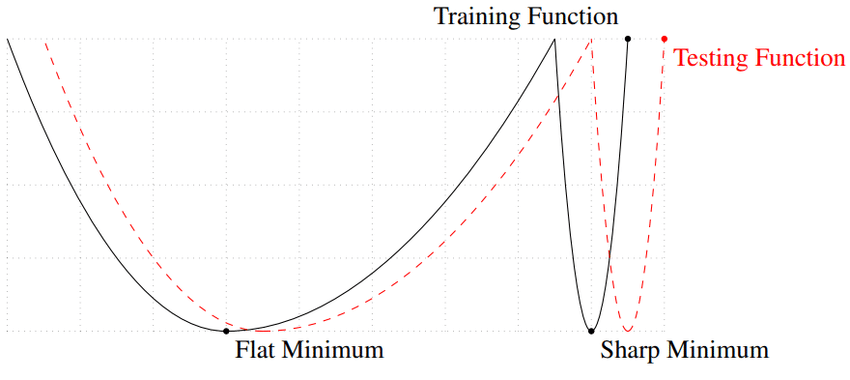
\includegraphics[width=0.5\textwidth]{imgs/generalization_loss.png}
\caption{ Los mínimos suaves supondrán, probablemente, cambios menores en el resultado del costo producto de las variaciones entre funciones de costo al variar los datos, y por ende presentan un \textbf{mayor poder de generalización} que los mínimos afilados. Fuente: \cite{fastbook} }
\label{fig:generalization_loss}
\end{figure}

\subsubsection{Descenso por gradiente estocástico}

Computar el gradiente del error sobre todo el conjunto de entrenamiento es costoso computacionalmente. En la actualidad los conjuntos de datos pueden ser muy grandes: ¡ya el conjunto de datos de imágenes \textit{ImageNet} (\cite{imagenet}) contiene 14 millones de imágenes de resolución considerable! (generalmente se trabaja con  recortes de 224x224 píxeles). Si se gasta demasiado tiempo para \textit{cada actualización} de los pesos el método sería demasiado lento.

Una solución consiste en estimar el gradiente de la función de costo $J$ teniendo en cuenta sólo un subconjunto de los datos de entrada (usualmente denominado \textbf{\textit{mini-batch}} $B$). Como ya dijimos, la función de costo depende de los datos. Podemos pensar, entonces, que estamos calculando el gradiente de la función de costo definida con ese subconjunto de datos $J_B$:

\begin{equation*}
    B \subset D_t
\end{equation*}
\begin{equation*}
    w \leftarrow w - \eta \nabla J_B(w)
\end{equation*}


Se particiona el conjunto de entrenamiento $D_t$ en \textit{mini-batches} y para cada uno se ejecuta un paso denominado \textbf{iteración de entrenamiento}: se evalúa el modelo, se calcula el gradiente del costo y se actualizan los pesos. 
Las iteraciones de todas las particiones constituyen lo que se denomina \textbf{época de entrenamiento}. 
La cantidad de épocas es la cantidad de veces que el modelo ajusta el conjunto de datos de entrenamiento, por lo que al aumentarlo hará más probable que el modelo comience a sobreajustar.

La elección del \textbf{tamaño del \textit{mini-batch}} supone una relación costo beneficio ya que a medida que lo incrementemos:
\begin{itemize}
    \item Cada iteración de entrenamiento consumirá más tiempo y memoria.
    \item El gradiente calculado $\nabla J_B(w)$ será más estable y representará una mejor estimación del gradiente verdadero $\nabla J(w)$ (sobre todo el conjunto de datos).
\end{itemize}

Como el subconjunto de datos que se le suministra al modelo en cada iteración de descenso por gradiente es aleatorio, el método se denomina \textbf{descenso por gradiente estocástico}. La estocasticidad introducida hace que $J_B$ sea distinto entre iteración e iteración y entre épocas sucesivas (ya que cambia $B$). Éstas variaciones suelen ser útiles para evitar mínimos filosos que no generalizan bien.

El hecho de entrenar en \textit{\textbf{mini-batch}} en vez de utilizar un único ejemplo no solo genera gradientes más estables (buenos estimadores del gradiente real) sino que se presta a paralelizar en \textbf{GPU} los cómputos: lo que ha permitido un enorme salto en el desarrollo del Aprendizaje Profundo.

\subsubsection{Importancia de la elección adecuada del \textit{learning rate}} \label{subsubsection:learning-rate}

La elección del \textit{learning rate} ha sido por tiempo uno de los hiperparámetros más importantes a la hora de entrenar redes neuronales. Como podemos ver en la figura \ref{fig:diff-lr}, de ser demasiado pequeño puede generar convergencia muy lenta y de ser demasiado grande también, e incluso, el proceso puede diverger.

\begin{figure}[h!]
\begin{subfigure}{0.33\textwidth}
\centering 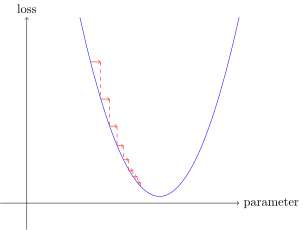
\includegraphics[width=0.3\textwidth]{imgs/lr_small.png}
\end{subfigure}
\begin{subfigure}{0.33\textwidth}
\centering 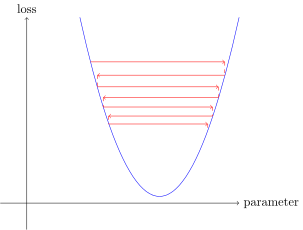
\includegraphics[width=0.3\textwidth]{imgs/lr_big1.png}
\end{subfigure}
\begin{subfigure}{0.33\textwidth}
\centering 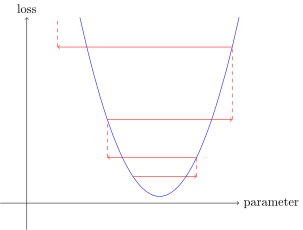
\includegraphics[width=0.3\textwidth]{imgs/lr_big2.png}
\end{subfigure}
\caption{ La elección del \textit{learning rate} es importante para la convergencia del método de manera eficiente. Fuente: \cite{fastbook} }
\label{fig:diff-lr}
\end{figure}


Más adelante se mostrarán optimizaciones más avanzadas que se basan en descenso por gradiente pero ajustan el \textit{learning rate} conforme avanza el entrenamiento. También existen heurísticas que permiten tomar decisiones razonables para la elección del mismo.

Es importante volver a resaltar que como la estabilidad de los gradientes calculados dependen del \textbf{tamaño de \textit{mini-batch}}, de éste dependerá el valor óptimo de \textit{learning rate}.

\subsection{Función de costo}

En el capítulo anterior asumimos que poseíamos una función que calculase el error para una asignación de parámetros determinada: 
\begin{equation*}
    J :  \mathbb{R}^{|W|} \rightarrow \mathbb{R}_0^+
\end{equation*}
A dicha función la nombramos \textbf{función de costo}. Luego introducimos un algoritmo para optimizarla, que se basa en el cálculo de $ \nabla J $. 

¿Por qué no usar las ya introducidas \textbf{métricas} como funciones de costo? 
Una de las razones es que sus gradientes no poseen buenas propiedades por lo que no se ajusta bien a nuestro algoritmo de aprendizaje.

Las métricas tales como la \textit{tasa de aciertos} son funciones escalonadas: un pequeño cambio en los pesos generará un cambio en las probabilidades de la predicción pero muy probablemente no cambiará la clase predecida, y por ende en la tasa de aciertos no se modificará. O sea el gradiente será nulo.

En cambio se utilizan como funciones de costo:
\begin{itemize}
    \item En problemas de \textbf{regresión} el ya definido \textbf{Error Cuadrático Medio} (\textbf{MSE}).
    
    Además de ser una función diferenciable, presenta buenas propiedades de concavidad.

    \item En problemas de clasificación binaria \textbf{\textit{Binary Cross Entropy}} \footnote{Centraremos nuestro análisis en \textit{BCE} ya que, como se dijo, el problema a tratar en este trabajo es de clasificación binaria. No obstante el concepto de \textit{BCE} se extiende fácilmente (y también sus propiedades) a la función de costo \textit{Cross Entropy Loss} para problemas de clasificación de cantidad arbitraria de clases.} (\textbf{BCE}):
    
    \begin{equation*}
        BCE(y, p) = \sum_{x_i \in D_v} y_i~log(p_i) + (1-y_i)~log(1-p_i)
    \end{equation*}
    
    \textbf{Observación:} como $y_i \in \{0,1\}$ (clasificación binaria), las expresiones $y_i$ y $1-y_i$ simplemente cumplen el rol de ``elegir'' que término sumar: $log(p_i)$ o $log(1-p_i)$ respectivamente.
    
    Intuitivamente podemos pensar que si el $log$ no estuviera es una \textit{``tasa de aciertos''} continua que mide que distancia hay entre la probabilidad predecida y la predicción correcta. El efecto del $log$ hace que la función pondere adecuadamente la diferencia entre clasificar, por ejemplo, con un error de $0.001$ y $0.01$ (en términos absolutos no es mucho pero en términos de error es $10 \times$ mejor).
    
    Es un caso particular de la función de entropía cruzada (en inglés \textit{Cross Entropy Loss}), utilizada en probabilidad para calcular diferencia entre distribuciones, con bases en la teoría de la información \cite{math-ml}.
    
\end{itemize}

Otro sustento matemático a la elección de dichas funciones de error es que sus fórmulas se derivan de los estimadores de máxima probabilidad (\textit{Max Likelihood Estimators}). 

\subsubsection{Linearidad de gradientes respecto a última capa de activaciones}

Una propiedad interesante surge de analizar $ \frac{\delta J}{\delta z} $ siendo $z$ la última capa de activaciones.\\

En problmeas de clasificación generalmente tendremos: \footnote{La nombrada \textit{función sigmoide} es una función de activación utilizada frecuentemente en la última capa para problemas de clasificación binaria. Se verá con más detalle en \ref{subsection:activaciones}. }
\begin{equation*}
    J(W) = BCE(y, sigmoid(z))
\end{equation*}
Y los gradientes respecto a la última capa de activaciones serán:
\begin{equation*}
    \frac{\delta J}{\delta z} = sigmoid(z) - y
\end{equation*}

En problemas de regresión simplemente será:
\begin{equation*}
    J(W) = MSE(y, z)
\end{equation*}
Y los gradientes respecto a la última capa de activaciones serán:
\begin{equation*}
    \frac{\delta J}{\delta z} = 2 (z - y)
\end{equation*}

En ambos casos los gradientes respecto a la última capa de activaciones serán proporcionales a la diferencia entre la predicción y el objetivo. 
Ésto hace que dicho gradiente que se ``propagará'' (como ya veremos en el capítulo de \textit{backpropagation}) hacia las capas anteriores no poseerá saltos bruscos: se \textit{suavizará} al aproximarse al objetivo tanto como se acerque al mismo. Sería problemático, si por el contrario aumentara exponencialmente al alejarse del objetivo, ya que, intuitivamente hablando, podría dar pasos tan grandes que saltase muy por ensima del mínimo y diverger (ver figura \ref{fig:diff-lr}). Notar que también sería un problema si no disminuyese conforme se acercase al mismo, ya que en un entorno próximo al mismo son necesarios pasos cada vez más pequeños.

\subsection{Funciones de activación} \label{subsection:activaciones}

Notar la importancia de aplicar funciones no lineales: de no hacerlo la combinación sucesiva de transformaciones afines no sería otra cosa que una transformación afín, y por lo tanto sería inútil la aplicación de sucesivas capas: el modelo sería en su conjunto una simple regresión lineal.

Diferentes funciones de activación utilizadas son:

\begin{figure}[h!]
\centering
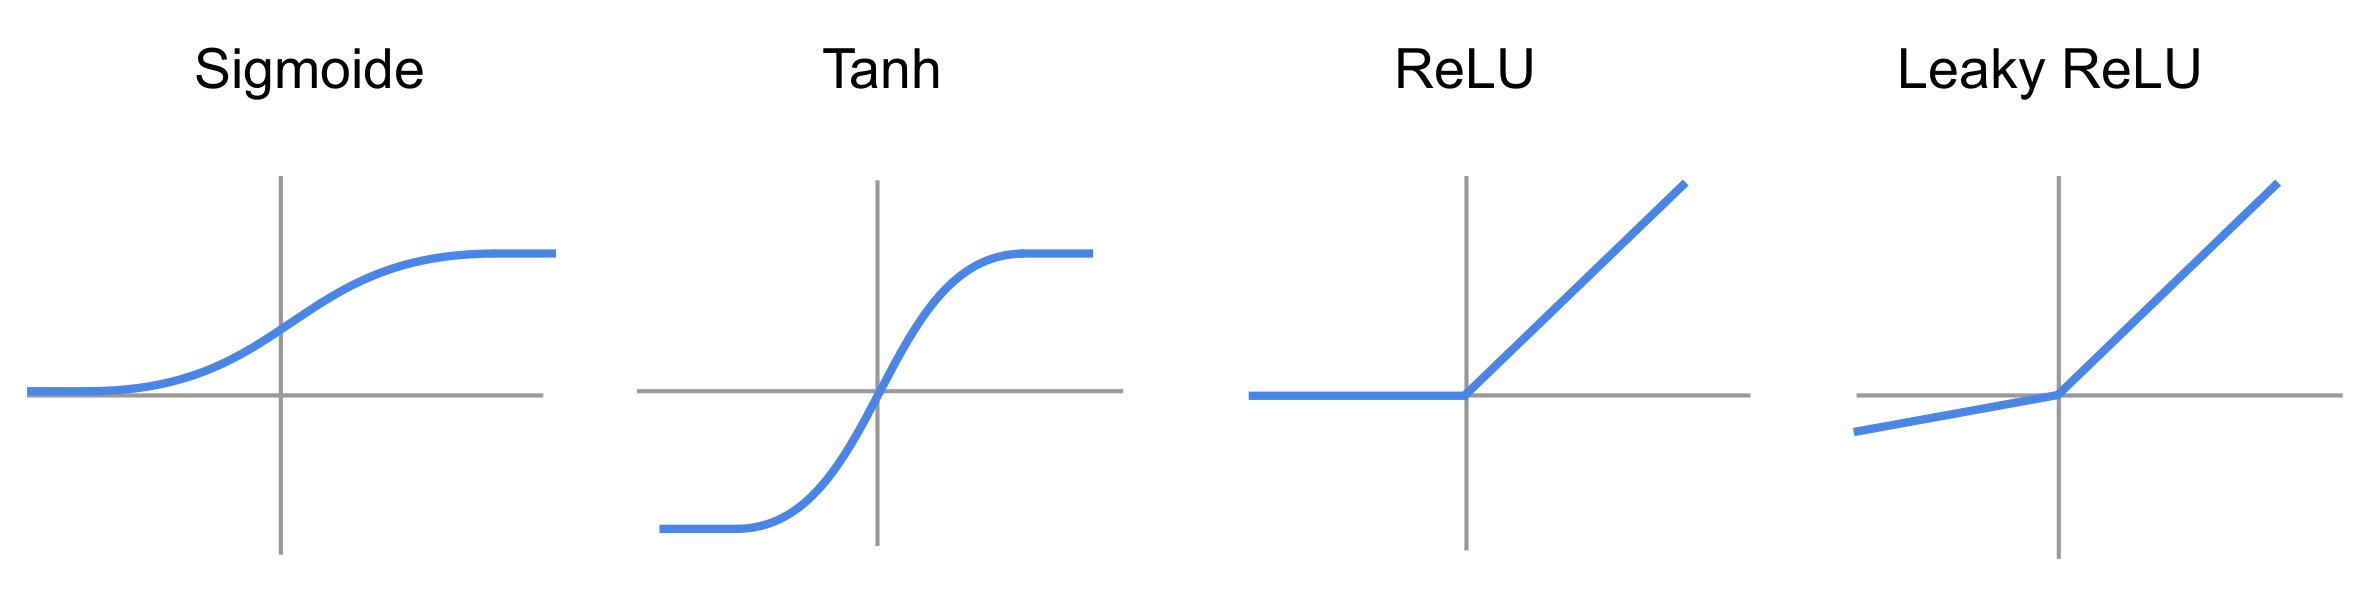
\includegraphics[width=0.8\textwidth]{imgs/activaciones.png}
\caption{ Diferentes alternativas para la función de activación. }
\label{fig:activaciones}
\end{figure}

\begin{itemize}
    \item \textbf{ Sigmoide }($\sigma$):
    \begin{equation*}
        \sigma(x) = \frac{1}{1+e^{-x}}
    \end{equation*}
    Las salidas de las neuronas sigmoideas no están centradas en el cero. Esto puede causar que el gradiente sea siempre positivo o negativo, causando inestabilidad en la actualización de los pesos.
    
    Suele utilizarse, no obstante, sobre la última capa de activaciones (como última función de activación) para problemas de clasificación binaria. De este modo las predicciones son números en el rango $[0,1]$ (consistentes con el hecho de reflejar probabilidades de pertenecer a la clase positiva o negativa). Además, como ya se explicó, posee buenas propiedades con respecto a \textit{BCE} al ser utilizada como última función de activación.
    
    \item \textbf{ Tangente hiperbólica }:
    \begin{equation*}
        tanh(x) = \frac{e^{x}-e^{-x}}{e^{x}+e^{-x}} = \frac{1}{1+e^{-2x}} - 1 = 2\sigma(2x) - 1
    \end{equation*}
    $Tanh$ es una sigmoide escalada y corrida. Resuelve el problema de centro distinto de cero.
    
    Históricamente estas dos funciones surgieron como primeras alternativas por ser diferenciables en todo su dominio, y en continuidad con el concepto de neurona encendida/apagada que poseía el perceptrón originalmente.
    
    Pero éstas funciones poseen el problema que el gradiente (derivada) es prácticamente nulo para valores de fuera del rango de [-2, 2]. Este problema se conoce como ``saturación del gradiente''.
    Ésto puede hacer muy pequeña la actualización de los pesos hacia capas anteriores (lo que se conoce como \textit{señal de backpropagation}) en los casos donde la activación escape al mencionado rango. Este comportamiento es denominado como problema de desvanecimiento del gradiente (en inglés, \textit{gradient vanishing}) y es sobretodo relevante en las actuales \textit{arquitecturas profundas} (que poseen un gran número de capas). Intuitivamente ``no les importa demasiado'' que los pesos de capas anteriores cambien ya que esto no genera cambios sustanciales en la función de activación. Es por eso que ya no se las utiliza como funciones de activación para capas intermedias. 
    
    \item \textit{\textbf{ Rectified Linear Unit}} (ReLU):
    \begin{equation*}
        ReLU(x) = max(0,x)
    \end{equation*}
    
    Las ReLUs fueron introducidas en \cite{relu-def} y sus variantes adquirieron mayor popularidad, mostrando resultados superadores en el entrenamiento de redes profundas debido a que:
    \begin{itemize}
        \item Resuelven el problema de saturación del gradiente.
        \item  Involucran operaciones simples (función $max(0,x)$ a diferencia de sigmoide o $tanh$ que involucran exponenciales), siendo computacionalmente menos costosas.
        \item En \cite{relu-fast} se muestra que son 6 veces más rápidas que sigmoide o $tanh$ para converger utilizando el método de descenso por gradiente estocástico.
        \item En \cite{relu-biology} muestran que las neuronas con ReLUs representan un mejor modelo de las neuronas biológicas y aprenden mejor que $tanh$ o sigmoide las representaciones dispersas.
        \item Es simple demostrar y ver (como veremos cuando hablemos de teorema de aproximación universal) que cualquier función puede ser aproximada como combinación lineal de ReLUs
    \end{itemize}

    Las ReLUs poseen un problema denominado ``neuronas muertas'': el gradiente es $0$ en el rango $(-\infty, 0)$ lo que anula la propagación a las capas anteriores y esto puede generar que conjuntos de neuronas de diversas capas no se activen. Y además, como tampoco actualizan sus respectivos pesos difícilmanete volverán a activarse.
    
    \textit{Leaky ReLU} introducidas en \cite{leaky-relu1} y \cite{leaky-relu2} pretende solucionar este problema agregando una pequeña pendiente en el rango $(-\infty, 0)$.

    
    \item \textit{\textbf{ Leaky ReLU}}:
    \begin{equation*}
        Leaky~ReLU(x) = \left\lbrace\begin{array}{c} \alpha x~si~x<0 \\  x~si~x \geq 0 \end{array}\right.
    \end{equation*}
    Con:
    \begin{equation*}
        0 < \alpha \ll 1
    \end{equation*}
    En general las ReLUs se siguen usando porque \textit{Leaky ReLU} no ha mostrado una mejoría consistente.
    
    \item \textit{\textbf{ Softmax}}: suele utilizarse en la última capa en problmeas de clasificación para transformar activaciones arbitrarias en probabilidades.
    
    \begin{equation*}
        \sigma : \mathbb{R}^K \rightarrow [0,1]^K
    \end{equation*}
    \begin{equation*}
        \sigma(z)_i = \frac{e_{z_i}}{\sum_{j=1}^K e_{z_j}}
    \end{equation*}
    
    Intuitivamente puede pensarse que:
    \begin{itemize}
        \item ``positiviza'' las activaciones y las mapea al rango $[0,1]$.
        \item  hace que la suma de las probabilidades sea $1$ (notar que sirve para problemas de clasificación donde la respuesta es una única clase, no múltiples clases).
        \item amplifica las diferencias entre las activaciones diferentes (tiende a tratar de escoger una única opción).
    \end{itemize}
    
    La elección de esta función tiene bases en la teoría de probabilidad. 
    
    El gradiente en la última capa de activaciones es lineal a la diferencia entre las predicciones y las etiquetas cuando se utilzia \textit{softmax} como última función de activación junto a \textit{BCE} como función de costo (al igual de lo que se mostró que pasaba con \textit{sigmoid}). Cómo se explicó, esto es una propiedad deseada.
    
\end{itemize}

\subsection{Teorema Aproximación Universal}

Como se dijo en la subsección \ref{subsection:intro-redes}, el Perceptrón de Rosenblatt de una sóla neurona cayó en olvido luego de que Marvin Mibsky mostrara que funciones simples como XOR no podían ser representadas. En la década del 80' las redes neuronales se popularizaron nuevamente luego que se demostrara que se podía solucionar dicho problema agregando más de una capa.

Los \textit{Teoremas de Aproximación Universal} son una familia de teoremas que demuestran las capacidadades de las redes neuronales de aproximar \textit{casi} cualquier función. 
No entraremos en detelle sobre la formulación matemática exacta de dichos teoremas (el lector interesado puede encontrar una explicación muy amena en el capítulo 4 de \cite{libro-nielsen}). 

Sólo nombraremos que se demuesta que es posible aproximar cualquier función continua en un espacio compacto de $\mathbb{R}^p$ a un grado de precisión arbitrario con:
\begin{itemize}
    \item \textbf{Dos capas + anchura arbitraria}: dado un número suficiente de neuronas intermedias.

    \item \textbf{Anchura limitada + profundida arbitraria}: con redes suficientemente profundas.
\end{itemize}
El primer caso es muy fácil de demostrar utilizando funciones de activación ReLUs. En la figura \ref{fig:universal-aprox} se muestra un esquema intuitivo. La idea subyacente es dividir el espacio compacto en intervalos y aproximar la función utilizando rectas adecuadas en cada intervalo. A su vez esto es fácil de lograr eligiendo e incorporando a la ecuación $ReLUs$ escaladas y corridas convenientemente para que generen dichas rectas lineales, siempre teniendo en consideración las $ReLUs$ ya elegidas.

\begin{figure}[h!]
\centering
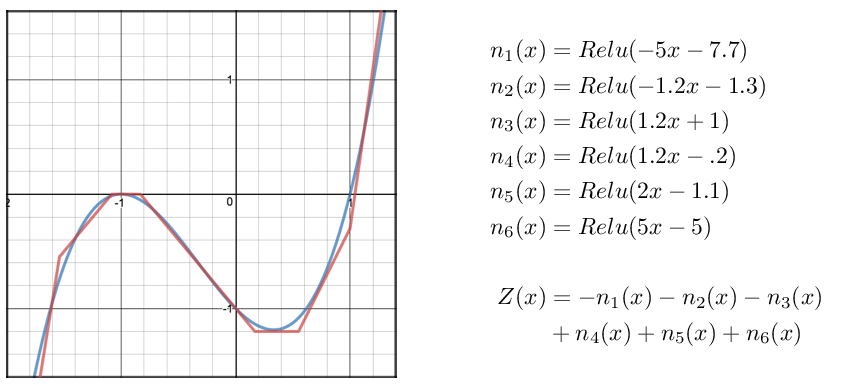
\includegraphics[width=0.8\textwidth]{imgs/universal_aprox.png}
\caption{ La imagen muestra la aproximación de un polinomio de tercer grado con una ``red de dos capas''. Fuente: \url{towardsdatascience.com/can-neural-networks-really-learn-any-function-65e106617fc6}. Autor: Brendan Fortuner }
\label{fig:universal-aprox}
\end{figure}

¡Notar que los teoremas no dan ninguna garantía de que el algoritmo de entrenamiento pueda aprendar esa función! E incluso siempre tendremos el limitante de la finitud de nuestros datos: no existe un procedimiento universal para elegir una función que generalice a puntos fuera del conjunto de entrenamiento \cite{limitation-aprox}.

Grandes errores se han cometido en el desarrollo del aprendizaje profundo por no entender que se trata de una disciplina práctica. En la década del 80' muchos científicos, en base al resultado de los teoremas de aproximación de dos capas, no experimentaron con redes más profundas. En la práctica éstas han mostrado una contundente mayor eficiencia produciendo resultados increíbles \cite{deeper-better}.

Debido al éxito de entrenar redes neuronales con muchas capas es que también nos referimos con un nombre propio al campo que estudia las redes neuronales profundas: \textbf{Aprendizaje Profundo},

\subsection{Algoritmo de \textit{backpropagation}}

En esta sección continuaremos explicando cómo se optimizan los parámetros. Explicaremos como se calculan los gradientes para cada peso siguiendo un algoritmo conocido como \textit{\textbf{backpropagation}}.\\

Ya se mostró que la arquitectura de nuestra red puede verse como composición sucesiva de funciones sobre los datos de entradas. Es natural entonces que para calcular los gradientes nos basaremos en la \textbf{regla de la cadena}. La misma nos dice que si tenemos:

\begin{equation*}
    E_1(w) = f(E_2(w))
\end{equation*}
Luego:
\begin{equation*}
    \frac{\delta E_1}{\delta w}(w) = \frac{\delta f}{\delta E_2}(E_2(w)) . \frac{\delta E_2}{\delta w}(w)
\end{equation*}
Utilizamos la notación de Leibinz extendida para resaltar en qué punto se evalúa cada derivada.\\

\textbf{Nota}: cuando hablamos de gradientes en redes neuronales nos referimos a \textit{valores} y no a las \textit{funciones}. A diferencia de lo que sucede en matemáticas donde es frecuente querer encontrar o calcular la función de gradiente o derivada, en cada iteración del entrenamiento, sólo necesitamos la derivada del error respecto a cada peso \textbf{aplicada en la asignación actual de pesos}.\\
  
En un principio, cuando las arquitecturas eran simples, dichas derivadas se calculaban con una fórmula codificada a mano para cada matriz $W^j$, $b^j$.  Pero si se observa con atención, la regla de la cadena nos da una forma inductiva de calcular los gradientes del error respecto de cada capa, haciendo uso de los gradientes ya calculados de capas posteriores.

Matemáticamente si tenemos las capas $f^1$, $f^2$ ... $f^n$ y las aplicamos sucesivamente según:
\begin{equation*}
    out = f^n ( ... f^2 ( f^1 (x) ) )
\end{equation*}
Y recordamos la notación para las activaciones tal como la definimos en la subsección \ref{subsection:nn-formulacion}:
\begin{equation*}
    \bar{h^0} = \bar{x}
\end{equation*}
\begin{equation*}
    \bar{h}^{j+1} = f^{j+1}(\bar{h}^j)
\end{equation*}

Luego podemos calcular los gradientes $\frac{\delta J}{\delta h^j}$ como:
\begin{equation*}
    \frac{\delta J}{\delta h^j} = \frac{\delta J}{\delta h^{j+1}}(h^{j+1}) . \frac{\delta h^{j+1}}{\delta h^j}(h^j)
\end{equation*}
Esta fórmula nos da una forma constructiva (algorítimica) de calcular los gradientes respecto de cada una de las activaciones, empezando por las capas más profundas (más cercanas al resultado) y conociendo la derivada $\frac{\delta h^{j+1}}{\delta h^j}(h^j)$ de la fórmula que computa una activación a partir de la anterior.  

Una vez que los gradientes respecto a cada capa ${h}^{j}$ han sido calculados, se puede computar de manera simple el gradiente respecto a los parámetros (pesos $W^j$ y \textit{biases} $b^j$) intervinientes en las respectiva capa. \cite{lecun-dl}. Simplemente, conociendo la derivada de $\phi^j$, podemos calcular $\frac{\delta J}{\delta W^j}$ y $\frac{\delta J}{\delta b^j}$ -en función del ya conocido $\frac{\delta J}{\delta h^j}$- valiéndonos de la fórmula de la capa:

\begin{equation*}
    \bar{h}^j = f^j(\bar{h}^{j-1}) = \phi^j( {W^j}^\top \bar{h}^{j-1} + b^j)
\end{equation*}

En éste cálculo la información fluye ``\textit{hacia atrás}'' y es por eso que se denomina \textbf{algoritmo de \textit{backpropagation}} \cite{backpropagation1}. En contraste a éste concepto se llama \textbf{\textit{forward propagation}} al cáclulo de las predicciones, ya que la información en este caso fluye ``\textit{hacia adelante}''.

Notar que en los cálculos intervienen los valores $h_j$, lo que significa que muchas veces será necesario guardar el valor de las activaciones (o al menos cierta información de ellas) para el cálculo posterior de los gradientes. \\

\textbf{Nota}: ¡El algoritmo de backpropagation es un caso de uso de programación dinámica! Estamos usando los resultados de instancias más chicas, o sea de las capas más cercanas al error, para calcular los casos ``más complejos'' de las capas menos profundas. \\

El mismo razonamiento es fácilmente generalizable a cualquier grafo acíclico de computaciones. Ésto es lo que usan los frameworks actuales para calcular los gradientes de manera transparente al usuario: en general no necesitaremos calcular ningún gradiente a mano. Cada una de las funciones definidas, definen un método para calcular los gradientes respecto de sus entradas utilizando como dato los gradientes respecto a esa misma capa. Los frameworks calculan un grafo de ejecucción que lleva el rastro de cómo se fue calculando determinado resultado. De modo que una vez calculado el error (o la función sobre la que queremos calcular los gradientes) es fácil calcular el gradiente de dicha función respecto cada capa (y luego de cada parámetro) haciendo uso de programación dinámica (\textit{backproapagation}) sobre el DAG de ejecucción que calculó el error. Ver esquema en la figura \ref{fig:dag}

\begin{figure}[h!]
\centering
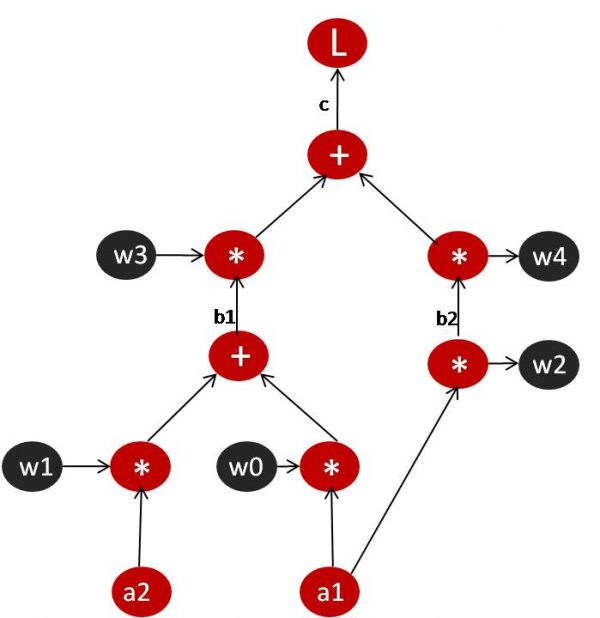
\includegraphics[width=0.4\textwidth]{imgs/autograd.jpg}
\caption{ Ejemplo de grafo de ejecucción construído en base al cálculo de un expresión. Créditos de la imágen: \url{mlearninglab.com/2019/04/14/autograd-una-de-las-claves-de-la-flexibilidad-de-pytorch/} }
\label{fig:dag}
\end{figure}

\subsection{Extensiones al algoritmo de descenso por gradiente}

En esta subsección explicaremos algunas optimizaciones que se hacen al algoritmo de descenso por gradiente estocástico para mejorar su estabilidad y convergencia. Las mismas, conforme avanza el entrenamiento, van adaptando y calculando valores que influyen en la actualización de los pesos. 

Generalmente estas optimizaciones ya vienen integradas en las bibliotecas que permiten crear y entrenar modelos de redes neuronales (como Pytorch y Tensorflow) y han sido utilizadas en el presente trabajo.

Notaremos $t$ al número de iteración y $w_t$ a los pesos al comienzo de la $t$-ésima iteración.

Una lista más extensa y comparaciones de las diferetnes optimizaciones se puede encontrar en \cite{compare-optimizers}.

\subsubsection{Momentum} \label{subsubsection:momentum}

Esta extensión fue propuesta en \cite{momentum}. Consiste en ``recordar'' información de las actualizaciones de pesos de iteraciones anteriores, calculando una media móvil exponencial de las actualizaciones $m_t$, ponderada por un hiperparámetro $\beta$:
\begin{equation*}
    m_t = \beta~m_{t-1} + (1-\beta) (- \eta~\nabla J(w_t))
\end{equation*}
\begin{equation*}
    w_{t+1} = w_t + m_t
\end{equation*}

Intuitivamente puede pensarse que el descenso por gradiente tendrá una \textit{inercia a la dirección que ya poseía}, de ahí que se lo llame \textbf{momentum} (por momento de inercia).

\subsubsection{RMSProp}

\textbf{RMSProp} (por \textit{Root Mean Square Propagation}) fue introducido por \cite{rmsprop}. Propone utilizar un \textit{learning rate} para cada parámetro de modo que los que \textit{``necesitan cambiar más''} posean valores más altos.

Esto lo logra mirando los gradientes, asumiendo que parámetros con gradientes más cercanos a 0 necesitan un \textit{learning rate} más alto para salirse de zonas planas. En cambio, si los gradientes son altos en valor absoluto significa que estamos en zonas empinadas, dónde conviene moderar el \textit{learning rate} para evitar divergencia. El factor que mide cuánto se tiene que reducir el \textit{learning rate} se lo nota $v_t$ (y es diferente para cada peso).

Para que $v_t$ no sea ruidoso (cambie demasiado entre iteraciones) y, en cambio, determinar una tendencia general del valor absoluto de los gradientes, se calcula la siguiente media móvil exponencial:


\begin{equation*}
    v_t = \beta v_{t-1} + (1-\beta) (\nabla J(w_t))^2
\end{equation*}
\begin{equation*}
    w_{t+1} = w_t - \frac{\eta}{\sqrt{v_t + \epsilon}} \nabla J (w_t)
\end{equation*}

Se agrega $\epsilon$ por razones de estabilidad numérica para evitar un denominador nulo.

\subsubsection{Adam} \label{subsubection:adams}

Debe su nombre a \textit{Adaptive Moment Estimation} y es una combinación de Momento y RMSProp propuesta en \cite{adam}. 

\begin{equation*}
    m_t = \beta_1 m_{t-1} + (1-\beta_1) \nabla J(w_t)
\end{equation*}

\begin{equation*}
    v_t = \beta_2 v_{t-1} + (1-\beta_2) \nabla (J(w_t))^2
\end{equation*}

Adam utiliza la media móvil no sesgada en su fórmula final. De modo que corrije el sesgo a $0$ existente en las medias móviles desde el inicio, al ser inicializadas en 0. Este sesgo es especialmente fuerte si $\beta_1$, $\beta_2$ son cercanos a 1 (como los valores que sugiere \cite{adam}). 

$\hat{m}_t$ y $\hat{v}_t$ son los estimadores no sesgados respecto a las medias móviles $m_t$ y $v_t$:

\begin{equation*}
    \hat{m}_t = \frac{m_t}{1-(\beta_1)^{t}}
\end{equation*}


\begin{equation*}
    \hat{v}_t = \frac{v_t}{1-(\beta_2)^{t}}
\end{equation*}

Finalmente la actualización de los pesos se calcula según:

\begin{equation*}
    w_{t+1} = w_t - \frac{\eta}{\sqrt{\hat{v}_t+\epsilon}} \hat{m}_t
\end{equation*}


\subsection{Inicialización de los parámetros}

Como explica el capítulo 17 de \cite{fastbook}, es importante la inicialización correcta de los pesos, sobretodo en redes profundas ya que se calculan muchas multiplicaciones sucesivas de las entradas con ellos. De inicializarlos muy pequeños (en valor absoluto) puede que las activaciones se anulen luego de sucesivas capas. Además, de iniciarlizarlos con valores absolutos demasiado altos (como las ReLU no limitan la saldia de cada capa), puede que incrementen exponencialmente el valor de las activaciones llegando a resultados computacionalmente inmanegables (valores \textit{nan}, de \textit{``not a number''}) causando errores de desbordameinto (\textit{overflow errors})

En \cite{xavier-init} se determina que la escala adecuada para inicializar los pesos es $\frac{1}{\sqrt{n_{in}}}$ siendo $n_{in}$ la cantidad de entradas de la capa. La \textbf{inicialización Xavier} inicializa los pesos en valores aleatorios con distribución gaussiana de media 0 y varianza $\frac{1}{\sqrt{n_{in}}}$.

Este factor depende del tipo de función de activación utilizada y \cite{xavier-init} lo han probado para $tanh$. En \cite{kaiming-init} (mismo trabajo que introduce las redes residuales) determina que la escala en caso de utilizar $ReLU$ es $\sqrt{\frac{2}{n_{in}}}$. Esta es la escala que utiliza el método de \textbf{inicialización Kaiming}.

\subsection{Mejorando la generalización - técnicas de regularización}

Otro desafío que supone el entrenamiento de redes neuronales es el del \textbf{sobreajuste}. Su gran complejidad, consecuencia de la gran cantidad de parámetros posibilita aprender funciones complejas pero también hace que sean más suceptibles a sobreajustar.

A veces se piensa -erróneamente- que la solución adecuada en estos casos es simplificar el modelo (reducir la cantidad de parámetros), la práctica del aprendizaje profundo desvela que es la última de las opciones a la hora de combatir el sobreajuste.

Existen una multitud de técnicas conocidas cómo \textbf{técnicas de regularización}, que permiten modificar el algoritmo de aprendizaje para producir modelos que generalicen mejor, sin achicar la cantidad de parámetros.

\begin{figure}[h!]
\centering
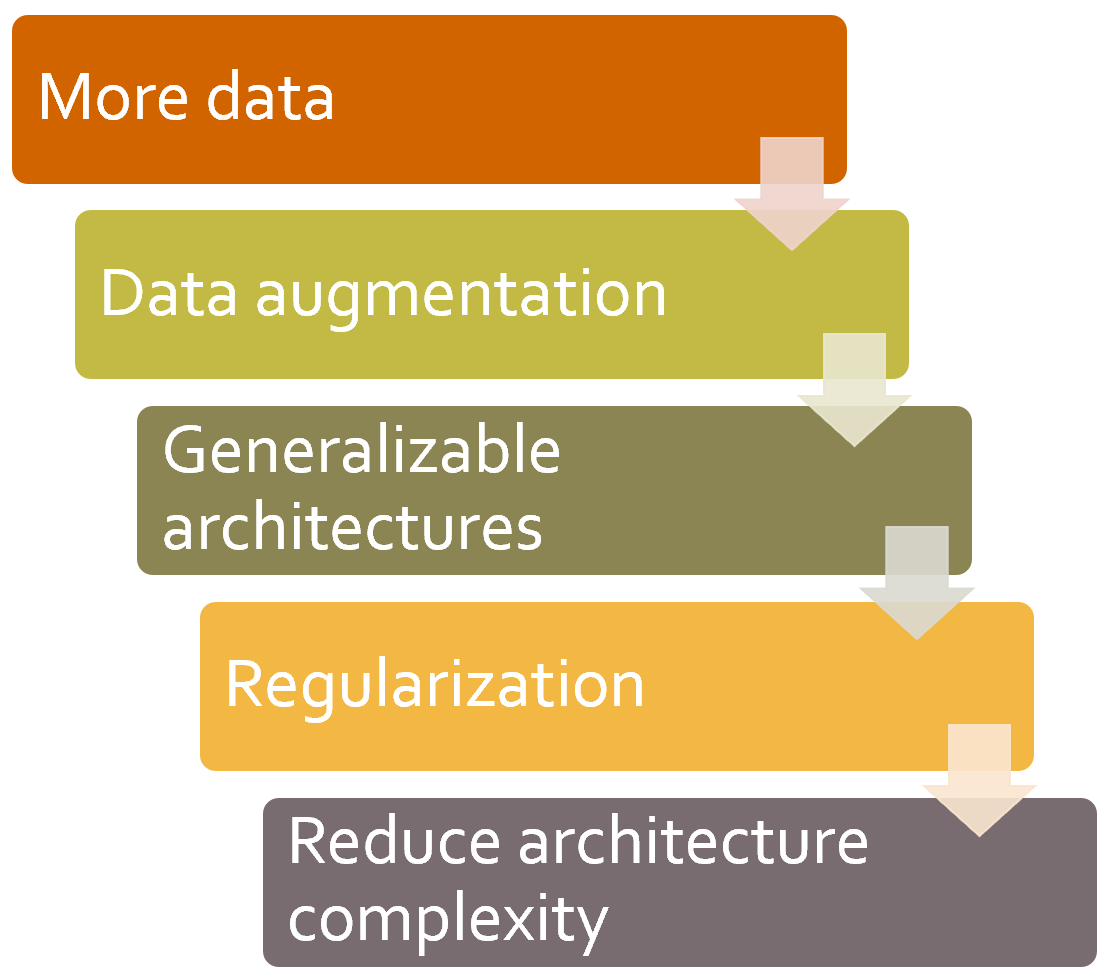
\includegraphics[width=0.5\textwidth]{imgs/overfitting_todo.png}
\caption{ \cite{fastbook} nos sugiere en su capítulo 5 seguir esta línea de acción ante el problema del sobreajuste. Fuente: \cite{fastbook}. }
\label{fig:overfitting_todo}
\end{figure}

En \cite{fastbook} se dice que si no podemos entrenar un modelo hasta que el mismo empiece a sobreajustar no estamos aprovechando en su totalidad la capacidad del mismo. 

También indica que la manera correcta de detectar el sobreajuste es \textbf{cuando el error de validación empieza a empeorar} (y no comparando el valor de la función de costo en el entrenamiento y la validación como muchos hacen). Después de todo, si el error de validación sigue disminuyendo y el conjunto de validación está bien confeccionado, significa que nuestro modelo está mejorando.

Ante la presencia del sobreajuste, reducir la complejidad del modelo tiene que ser la última opción en redes neuronales (ver figura \ref{fig:overfitting_todo}): \cite{fastbook} sugiere intentar antes con técncias de \textit{data augmentation}, agregar regularización en la arquitectura (como capas de \textit{batch normalization} y \textit{dropout}) y aumentar luego los valores de regularización (incrementar los hiperparámetros que influyen en ella como $\lambda$ de \textit{weight decay}, o el $p$ de las capas de \textit{dropout}). Todas estas técnicas se verán en las subsecciones siguientes.

\subsubsection{\textit{Data augmentation}}

El proceso de \textit{\textbf{Data Augmentation}} consiste en generar datos sintéticos durante la fase de entrenamiento. Muy a menudo al contar con pocos datos, el modelo ajustará demasiado los datos de entrenamiento disponibles, lo que dará lugar (como ya se ha explicado en secciones anteriores) al sobreajuste.

Existen métodos de generar datos sintéticos que son dependientes de la naturaleza de los datos. Por ejemplo en el caso de imágenes es común generar más datos aplicando transformaciones como rotación, traslación, escalamiento, espejamiento o diferentes tipo de deformación mientras que no cambien sustancialmente la semántica de la imágen (ver ejemplo figura \ref{fig:data-augmentation-image-fastai}). Estas transformaciones son combinables. Debe tenerse en cuenta que tengan sentido en el contexto del problema elegido. Por ejemplo si estamos reconociendo objetos espejar es una operación válida, mientras que si estamos reconociendo texto no lo será.

\begin{figure}[h!]
\centering
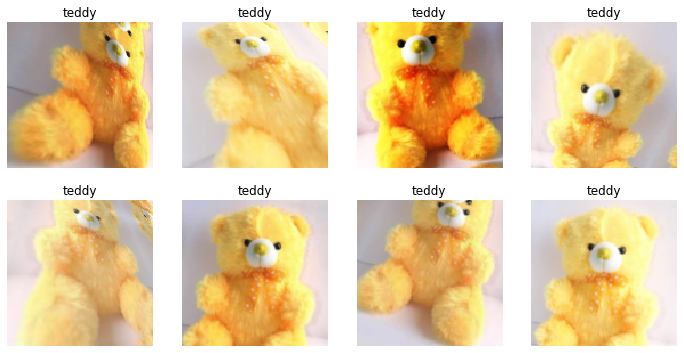
\includegraphics[width=0.6\textwidth]{imgs/data_augmentation.png}
\caption{ La librería fastai provee una forma de realizar \textit{Data Augmentation} en la GPU, acelerando considerablemente el entrenamiento. Fuente: \cite{fastbook}.  }
\label{fig:data-augmentation-image-fastai}
\end{figure}

También existen métodos estadísticos generales de \textit{data augmentation}. Por ejemplo el agregado de ruido en función a la distribución de los datos, que son aplicables a diversos tipos de datos (imágenes, sonido, vector de características, etc). Además existen métodos más avanzados como las Redes Generativas Adversiales capaces de aprender la distribución intrínseca de los datos, y a partir de ello generar datos sintéticos.\\

\begin{figure}[h!]
\centering
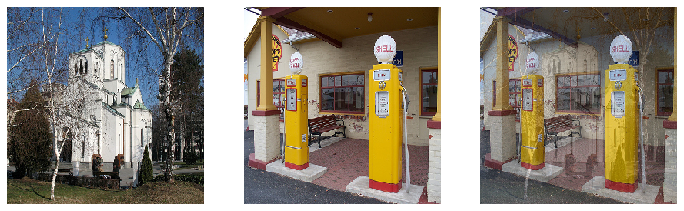
\includegraphics[width=0.6\textwidth]{imgs/mixup_result.png}
\caption{ Un ejemplo de la técnica \textit{Mixup} que combina ponderadamente dos imágenes (estación de gasolina y templo). Fuente: \cite{fastbook}  }
\label{fig:data-augmentation-mixup}
\end{figure}

Un método simple que arroja muy buenos resultados en problemas de clasificación, utilizado en Aprendizaje Profundo, es la técnica de \textbf{Mixup}  \cite{mixup} que consiste en generar nuevos ejemplos a partir de hacer un promedio ponderado entre dos datos (ver ejemplo figura \ref{fig:data-augmentation-mixup}). El mismo promedio, con igual ponderación, se aplica a las etiquetas para generar una nueva etiqueta sintética respectiva. Ver formulación matemática en la figura \ref{fig:data-augmentation-mixup-formula}.

\begin{figure}[h!]
\centering
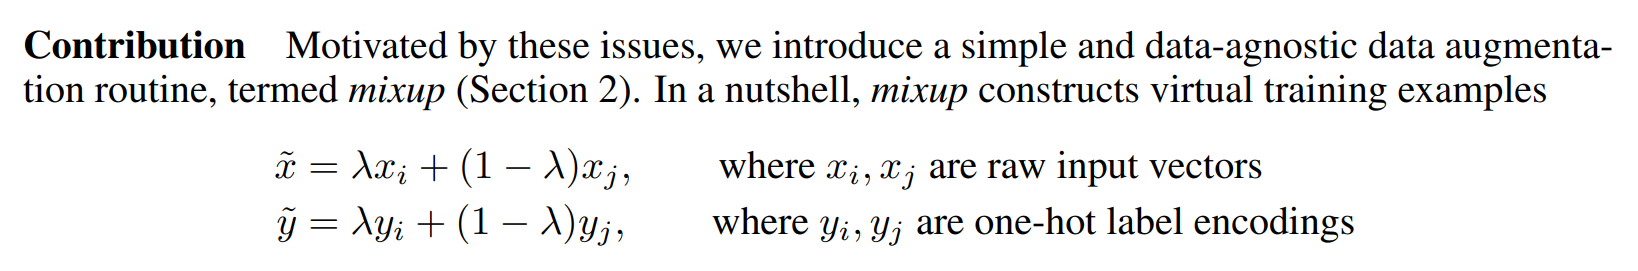
\includegraphics[width=1\textwidth]{imgs/mixup_formula.png}
\caption{ La formulación matemática de \textit{Mixup} según \cite{mixup}.  }
\label{fig:data-augmentation-mixup-formula}
\end{figure}

\subsubsection{\textit{Batch normalization}} \label{subsubection:batch-normalization}

Un problema que causa entrenamientos infecientes es el denominado \textit{\textbf{``internal covariance shift''}} explicado en \cite{batch-normalization}: la entrada de cada capa cambia conforme se entrenan las capas anteriores, por lo cuál le costará aprender los pesos definitivos hasta que las capas anteriores hayan \textit{convergido suficientemente}. Podemos pensar intuitivamente que desde la perspectiva de cada capa es como si \textit{``le cambiaran el conjunto de datos''} todo el tiempo.

Una ingeniosa manera de ver esto es en las gráficas propuestas en el capítulo 13 de \cite{fastbook} donde se grafica mediante mapa de color los histogramas de los valores de activación en función a iteraciones de entrenamiento. Como se puede ver en la figura \ref{fig:histogramactivation} las activaciones comienzan casi todas en cero. Luego, cíclcicamente, incrementan su valor exponencialmente y vuelven a cero (como si volvieran a comenzar).

\begin{figure}[H]
\begin{subfigure}{0.45\textwidth}
\centering  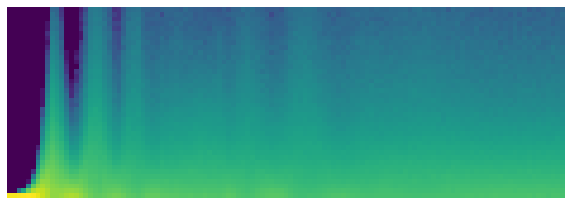
\includegraphics[width=0.8\textwidth]{imgs/histogram_activation1.png}
\end{subfigure}

\begin{subfigure}{0.45\textwidth}
\centering 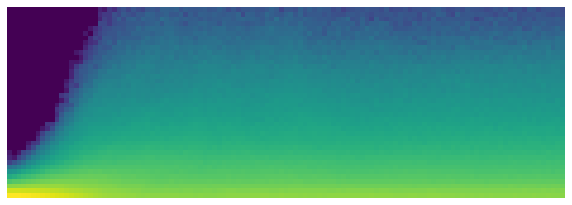
\includegraphics[width=0.8\textwidth]{imgs/histogram_activation2.png}
\end{subfigure}

\caption{ Se grafica para cada valor de activación (eje y) su cantidad en un hisotrama (color, el cero corresponde a colores más oscuros), conforme avanzan las iteraciones (eje x). En la primer figura se muestra un entrenamiento sin regularización. Se puede observar como las activaciones aumentan muy velozmente y vuelven a cero cíclicamente. En la segunda figura, luego de aplicar \textit{batch normalization}, este comportamiento desaparece: el aumento de los valores de las activaciones es más lento y consistente.  Fuente: capítulo 13 de \cite{fastbook}.  }

\label{fig:histogramactivation}
\end{figure}

Como solución a eso \cite{batch-normalization} propone normalizar cada capa de activaciones para que tengan media 0 y varianza 1. De modo de reducir ese cambio en la varianza de capas internas (\textit{internal covariate shfit}). Sobre la salida de activaciones $h_i$ de cada mini-batch se calcula su media $\mu$ y varianza $\sigma^2$ y se normaliza según:

\begin{equation*}
    BN(h_i) = \frac{h_i - \mu }{\sigma}
\end{equation*}

Para no limitar la capacidad del modelo a producir activaciones más grandes, se introducen dos parámetros \textit{entrenables} $\gamma$ y $\beta$. Serán optimizados por el método de entrenamiento como cualquier otro peso. Así se permite \textit{aprender} la media y varianza de la salida:

\begin{equation*}
    out_i = \gamma~BN(h_i)  + \beta
\end{equation*}

El método de Batch normalization hace más estable el entrenamiento, permitiendo incrementar el \textit{learning rate} y entrenar más rápidamente (menos iteraciones). También parece generar modelos que generalizan mejor, probablemente por la introducción de estocasticidad (que el modelo tiene que superar volviéndose más robusto) por la variabilidad de $\mu$ y $\sigma^2$ de las activaciones entre diferentes \textit{mini-batches}.

En el figura \ref{fig:histogramactivation} es evidente el cambio en la estabilidad de las activaciones conforme avanzan las iteraciones luego de aplciar \textit{batch normalization}.

\subsubsection{\textit{Weigth decay}} \label{subsubsection:wd}

Técnica introducida por \cite{weight-decay} que consiste en añadir un término al error que penalice la suma de los cuadrados de los pesos:
\begin{equation*}
    J_{Weight~Decay}(W) = J(W) + \lambda \sum W_i^2
\end{equation*}

$\lambda$ es un hiperparámetro que controlará la cantidad de penalización aplicada. Valores más altos entorpecerán un poco más nuestro entrenamiento pero harán que el modelo resultante generalice mejor.

Esto incentiva elegir pesos pequeños. La razón detrás de ello es que pesos grandes generan mínimos afilados en la función de costo que, como se mostró, generalizan mal. Un argumento intuitivo se expone en la figura \ref{fig:weight-decay}.

\begin{figure}[h!]
\centering
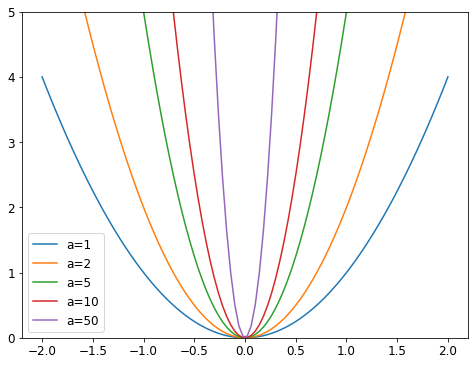
\includegraphics[width=0.6\textwidth]{imgs/weight_decay.png}
\caption{ Al aumentar $w$ en la fórmula $w x^2$ la parábola se vuelve más ``afilada''. Fuente: capítulo 8 \cite{fastbook}. }
\label{fig:weight-decay}
\end{figure}

Es fácil ver que el término de penalización en la función de costo agregará un término de $2 \alpha W_i$ sobre los gradientes de cada peso. En la práctica no se añade explícitamente el término a la función de costo sino que se modifica el cálculo de la actualización de los pesos agregando un factor de $W_i$:
\begin{equation*}
    \Delta W_i = - \eta \nabla J(W)_i - \eta \lambda w_i
\end{equation*}
O también se lo puede agregar en el cálculo del gradiente:
\begin{equation*}
    \nabla \hat{J}(W)_i = \nabla J(W)_i + \lambda w_i
\end{equation*}
Ambas son equivalentes para el método de descenso por gradiente estocástico pero en el trabajo desarrollado por \cite{decouple-weight-decay} se recomienda la segunda cuando se aplica en combinación con las técnicas momentum o Adam, debido a que es más fiel a la formulación original, y también muestra mejores resultados prácticos.

\subsubsection{\textit{Dropout}}

Es una técnica de regularización introducida en \cite{dropout}  que consiste en desactivar aleatoriamente ciertas neuronas (llevando su respectiva activación a $0$) durante el entrenamiento. Ver figura \ref{fig:dropout}.

\begin{figure}[h!]
\centering
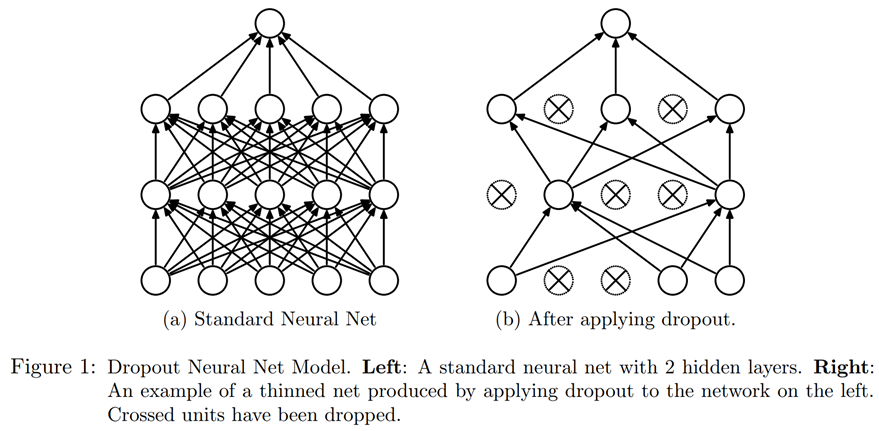
\includegraphics[width=0.9\textwidth]{imgs/dropout.png}
\caption{ Imagen esquemática extraída de \textit{``Dropout: A Simple Way to Prevent Neural Networks from Overfitting''} \cite{dropout}. }
\label{fig:dropout}
\end{figure}


La técnica funciona asombrosamente bien y ha generado un salto en el estado del arte del aprendizaje profundo. La intuición detrás de ella es que:
\begin{itemize}
    \item Mejora la cooperación entre neuronas impidiendo que intrincadamente neuronas de diferentes capas aprendan funciones de ``memorización'' del conjunto de entrenamiento. Incentivando que aprendan a extraer verdaderas características útiles y robustas.
    \item Introducen ruido en las activaciones, haciendo que se aprendan características más robustas en cada capa.
\end{itemize}

El \textit{dropout} se aplica sobre determinadas capas e incluso se ha mostrado su utilidad aplicándolo sobre la entrada para introducir ruido. Ésto puede pensarse como un caso de \textit{data augmentation}.

Notar que el apagado de las neuronas de una capa con probabilidad $p$  durante el entrenamiento requiere que se escale las salidas restantes en $\frac{1}{1-p}$. De lo contrario la capa posterior recibiría en promedio $p$ activaciones en 0 más durante el entrenamiento que durante fase de validación o durante la inferencia, lo que generaría diferentes valores promedios de activación en el entrenamiento respecto de validación, y arruinaría totalmente la generalización.

\subsection{Configurando el \textit{Learning Rate}}

Como se explicó en el apartado \ref{subsubsection:learning-rate}, el \textit{learning rate} es uno de los parámetros más importantes en el Aprendizaje Profundo: de ser muy pequeño el modelo puede tardar demasiado en entrenar, y de ser muy grande el entrenamiento puede diverger.

Optimizadores tales como Adam (explicado en el apartado \ref{subsubection:adams}) permiten escalarlo adecuadamente según el valor del gradiente. Pero notar que aún utilizando Adam, es necesario la elección del \textit{learning rate} inicial. Siendo el escalamiento aplicado por Adam independiente del valor inicial elegido.

Otras optimizaciones como \textit{Batch Normalization} (apartado \ref{subsubection:batch-normalization}) y \textit{Weight Decay} (apartado \ref{subsubsection:wd}), mitigan los riesgos de divergencia existentes derivados de utilizar valores de \textit{learning rate} elevados. No obstante, no resuelven el problema de escoger un valor inicial.

\subsubsection{Seteando el \textit{Learning Rate} inicial}

Cansado de que el modo de hallar el \textit{learning rate} óptimo sea cuestión de prueba y error, generalmente utilizando métodos como \textit{Grid Search} que requieren re-entrenar el modelo varias veces (consumiendo demasiado tiempo), Leslie N. Smith\footnote{\textbf{Nota:} Leslie N. Smith se doctoró en Química Cuántica en la Universidad de Illinosis y es investigador del \textit{Naval Research Laboratory} de los Estados Unidos. Se introdujo al Aprendizaje Profundo en 2013 y sus estudios han contribuído en hallar técnicas para entrenar más rápido y con menos datos. Este es un paso fundamental a la hora de democratizar la Inteligencia Artificial y volverla más accesible a más personas (y no solo un puñado de grandes compañías). Veáse esta entrevista que hizo para Jeremy Howard: \url{youtube.com/watch?v=dxpyg3mP_rU}}, en \cite{lr-finder}, describe un ingenioso método para encontrar el \textit{learning rate} inicial que denominó \textit{Range Test}. \footnote{También es conocido bajo el nombre de \textit{Learning Rate Finder} por la biblioteca de Aprendizaje Profundo FastAI, la cual popularizó el método usándolo en su implementación. }
El mismo consiste en probar \textit{learnings rates} incrementales (desde un valor pequeño como $10^4$) e ir aumentándolo conforme avanzan las iteraciones (para siguientes \textit{mini-batches}) hasta que el valor de la función de costo empieze a aumentar demasiado indicando divergencia (ver figura \ref{fig:lrfinder}). Luego, se corrobora empíricamente que un buen \textit{learning rate} inicial resulta de elegir un orden de magnitud por debajo del mínimo o un valor luego del cual se presente una caída abrupta del costo. Intuitivamente, para este valor la función de costo sigue decreciendo.

\begin{figure}[h!]
\centering
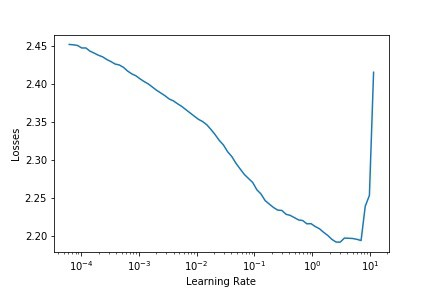
\includegraphics[width=0.6\textwidth]{imgs/lrfinder.jpeg}
\caption{ La librería FastAI provee un método denominado \textit{Learning Rate Finder} que ejecuta el test descripto en \cite{lr-finder} y muestra la gráfica de la función de costo a medida que se aumenta el \textit{learning rate}. En este caso particular una elección de \textit{learning rate} posible oscila entre $10^{-1}$ y $0.5$ (un orden de magnitud menor que el mínimo). Fuente: \href{https://github.com/fastai/fastai}{fastai}  }
\label{fig:lrfinder}
\end{figure}

\subsubsection{\textit{Cycle Learning Rates}}

Una técnica utilizada es hacer descender el \textit{learning rate} a medida que avanza el número de iteraciones, intuitivamente, para que al acercarse al minimo no se ``saltase'' por ensima de él.

En \cite{lr-finder} se sugiere hacer oscilar el valor del \textit{learning rate}, en cada época, entre dos umbrales (ver figura \ref{fig:clr}). La experimentación muestra que así se logran convergencias más rápidas.

\begin{figure}[h!]
\centering
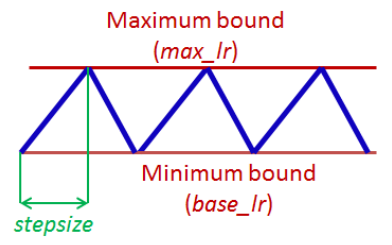
\includegraphics[width=0.4\textwidth]{imgs/clr.png}
\caption{ Imagen esquemática extraída de \cite{lr-finder}. Se halla empíricamente que incrementando y decrementando cíclicamente el \textit{learning rate} se obtienen entrenamientos más veloces y modelos que generalizan mejor.   }
\label{fig:clr}
\end{figure}

Una de las razones intuitivas es que permite superar puntos de ensilladura (ver ejemplo figura \ref{fig:saddle}). Los puntos de ensilladura son un obstáculo para el método de descenso por gradiente, ya que son zonas planas, difíciles de superar, y por ende, donde el entrenamiento se ve realentizado. Además, según reporta \cite{ensilladura}, son mucho más frecuentes que los mínimos locales en las topologías de funciones de costo.

\begin{figure}[h!]
\centering
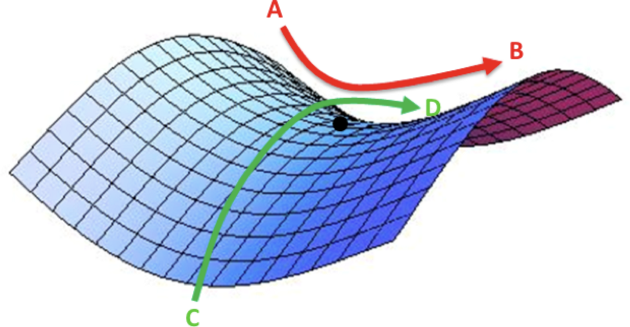
\includegraphics[width=0.4\textwidth]{imgs/saddle.png}
\caption{ Punto ensilladura para una entrada 2-dimensional. Créditos de la imágen \href{https://www.safaribooksonline.com/library/view/fundamentals-of-deep/9781491925607/ch04.html}{safaribooksonline} }
\label{fig:saddle}
\end{figure}

En \cite{leslie-2}, se ha reportado mejoras significativas en la velocidad de entrenamiento aplicando ésta técnica (utilizando en CIFAR-10 y CIFAR-100 y la familia de ResNets). El autor ha denominado a este fenómeno ``Super - Convergencia''. \cite{leslie-3}

\subsubsection{\textit{One Cycle Policy}}

Finalmente en \cite{leslie-final}, L. Smith sugiere un política de único cíclo por época para variar el \textit{learning rate}: comenzando con valores pequeños, aumentando al principio del ciclo y disminiyéndolo sobre el final (ver figura \ref{fig:one-cycle}.a). Además fija el tamaño del ciclo un poco menor al número de iteraciones de una época, y en las últimas iteraciones disminiye progresivamente el \textit{learning rate} hacia 0 (esta idea está inspirada en \textit{``Simulated Annealing''} \cite{sa}).


\begin{figure}[h!]
\begin{subfigure}{0.45\textwidth}
\centering 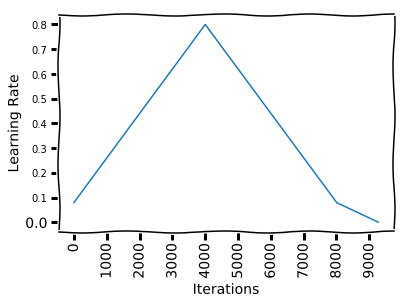
\includegraphics[width=0.45\textwidth]{imgs/onecycle_lr.png}
\end{subfigure}
\begin{subfigure}{0.45\textwidth}
\centering 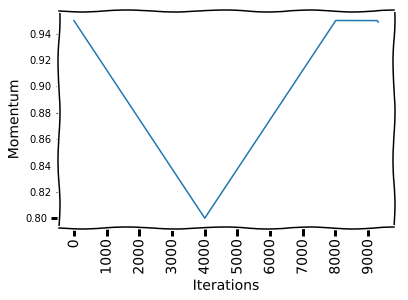
\includegraphics[width=0.45\textwidth]{imgs/onecycle_momentum.png}
\end{subfigure}
\caption{ En la imágen podemos observar cómo varía el \textit{learning rate} (izquierda) y \textit{momentum} (derecha) según la Política de Único Cíclo descripta en \cite{leslie-final}. Créditos de la imágen: \href{https://towardsdatascience.com/finding-good-learning-rate-and-the-one-cycle-policy-7159fe1db5d6}{\textit{``Finding Good Learning Rate and The One Cycle Policy''}}, autor Nachiket Tanksale.}
\label{fig:one-cycle}
\end{figure}

En \cite{leslie-final} se corroboran mejores resultados de variar el \textit{momentum} de manera inversa a la variación del \textit{learning rate}: comenzando por el umbral máximo, reduciéndolo y luego aumentándolo (ver figura \ref{fig:one-cycle}.b). Para finalmente utilizar el valor máximo de \textit{momentum} para la fase de \textit{annealing} del \textit{learning rate}

La intuicion detrás de ello es que en los momentos donde el \textit{learning rate} se está aumentando para superar puntos de ensilladura, uno desearía que el algoritmo de descenso por gradiente rápidamente vaya hacia nuevas direcciones, para lo cual es necesario que tenga baja inercia. 
 
Otra forma de entender por qué es razonable variar el \textit{momentum}, se desprende de observar la fórmula del mismo (presentada en el apartado \ref{subsubsection:momentum}) y notar que $1-\beta$ ($\beta$ es el \textit{momentum}) tiene un impacto similar a $\lambda$ (\textit{learning rate}) en la actualización de los pesos:

\begin{equation*}
    m_t = \beta~m_{t-1} + (1-\beta) (- \eta~\nabla J(w_t))
\end{equation*}

Por lo que es razonable que si en nuestra política variamos $\lambda$ querremos que $\beta$ variase en sentido opuesto (y que no nos ``contrarreste'' la variación).\\

En \cite{leslie-final} se reportan mejoras en la velocidad de entrenamiento de \textit{ResNet-50} para el dataset CIFAR-10 y CIFAR-100 de hasta $\times 10$. Además se obseva que los modelos generalizan mejor (presentan mejores resultados de validación). Esto es atribuído, a que entrenando con \textit{learnings rates} más altos se encuentran mínimos más suaves, ya que de encontrar uno empinado probablemente se ``salte'' fuera del mismo. Como se explicó en el apartado \ref{subsubsection:sharped-mins} los mínimos suaves generalizan mejor. Una vez que -aumentando progresivamente el \textit{learning rate} para evitar divergencia- se encuentran zonas con mínimos más suaves, la fase de disminución progresiva hace que encontremos la mejor parte de dicha zona (la de menor costo).

\subsection{Aprendiendo las representaciones} \label{subsection:representaciones}

Anteriormente al Aprendizaje Profundo los sistemas solían tener una fase de extracción de características que luego eran suministradas a un algoritmo de Aprendizaje Automático para entrenar \cite{dlpytorch}. La primer fase era dependiente del dominio: necesitaba ingeniería de características propia para cada problema (para imágenes se utilizaban filtros detectores de bordes, cantidad de agujeros, etc).

Por el contrario, en el Aprendizaje Profundo las características adecuadas son \textit{aprendidas} (calculadas automáticamente) por el modelo mismo. El cual, a medida que es entrenado, produce mejores características. Usualmente las representaciones aprendidas son mejores que las que puede escribir un experto manualmente. Ver figura \ref{fig:aprender-representaciones}.

\begin{figure}[h!]

\centering
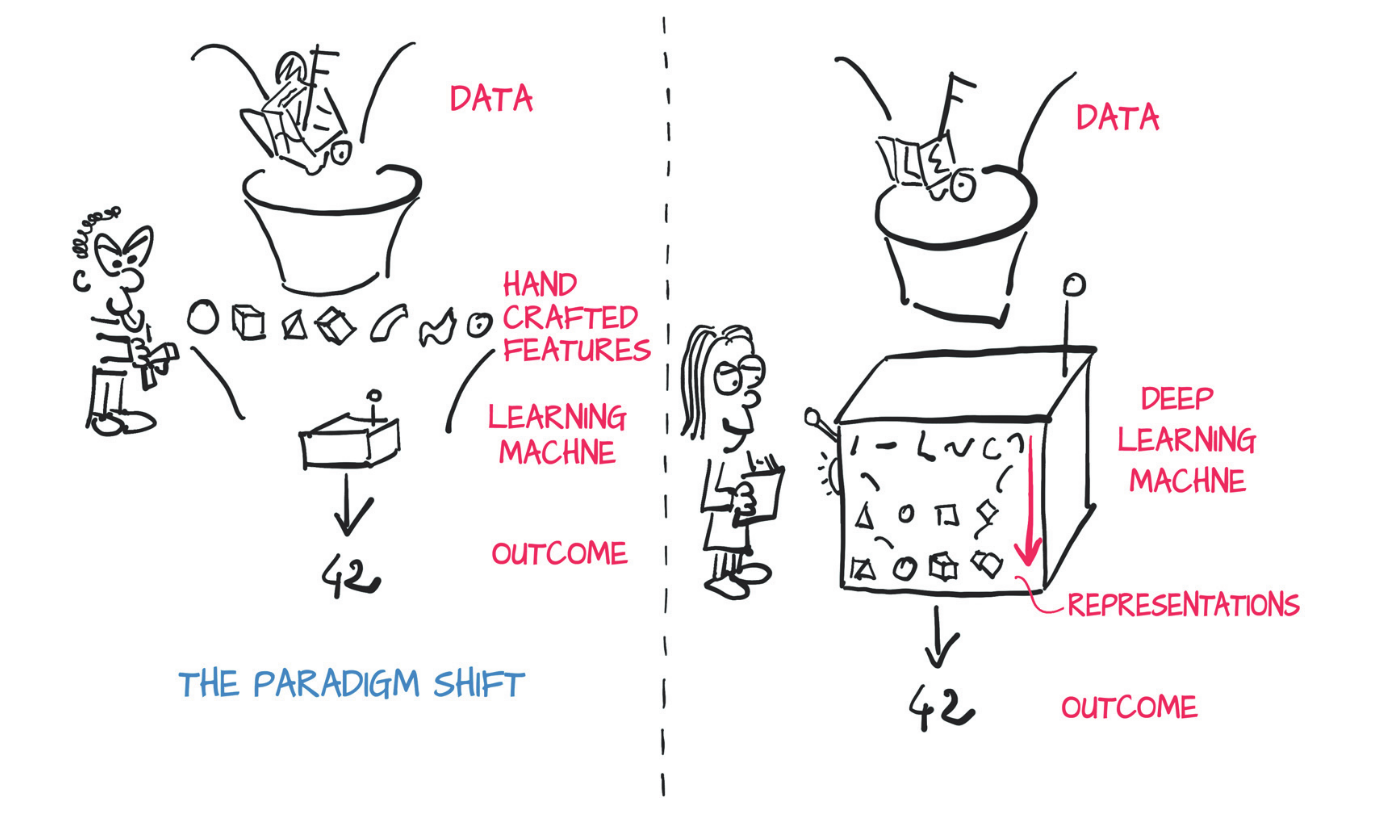
\includegraphics[width=0.65\textwidth]{imgs/learningfeatures.png}

\caption{ Imagen que esquematiza el cambio de paradigma en el Aprendizaje Automático: a la izquierda un experto del dominio se ocuapaba de programar manualmente la extracción de características. A la derecha, con el paradigma del Aprendizaje Profundo, puede focalizarse en que el modelo entrene adecuadamente para aprendarlas. Fuente: \cite{dlpytorch}}
\label{fig:aprender-representaciones}
\end{figure}

El hecho de contar con Redes Neuronales de muchas capas posibilita que las primeras aprendan representaciones más básicas, sobre las cuáles se basen las representaciones más refinadas de las capas subsiguientes. Posibilitando un paradigma que consiste en suministrarle los datos crudos al modelo (por ejemplo los píxeles de la imágen) y que no sea necesario conocimiento específico del dominio para realizar la extracción de características manualmente. Haciendo así mucho más fácilmente trasladable los métodos entre diferentes dominios de aplicación.

Éste ha sido la clave del éxito del Aprendizaje Profundo y lo que ha popularizado a las Redes Neuronales. Y fue posible gracias a que se empezó a experimentar con más de una sóla capa oculta. 

Los siguientes factores han sido clave en el desarrollo de las Redes Neuronales profundas:
\begin{itemize}
    \item El aumento en la capacidad de cómputo (sobretodo el uso de GPU).
    \item Atreverse a experimentar con más de una capa oculta (pese a las malas interpretaciones del Teorema de Aproximación Universal).
    \item El surgimiento de arquitecturas con conexiones más dispersas entre capas sucesivas: las Redes Convolucionales (que se verán en la siguiente sección), que posibilitó agregar más capas con menor costo computacional.
\end{itemize}


\subsection{Redes Neuronales Convolucionales}

Nuestro trabajo se enfocará en \textbf{Redes Neuronales Convolucionales} (\textit{CNN} del inglés \textit{Convolutional Neural Network}), arquitectura que posibilitaron modelos muy profundos de Redes Neuronales, constituyendo el primer gran éxito del Aprendizaje Profundo \cite{lenet}.\\

Se basan en dos observaciones claves, particularmente válidas para problemas de análisis de imágenes: 
\begin{itemize}
    \item Las características son \textit{locales}.  La salida de cada capa puede ser construída teniendo en cuenta solamente un área acotada de la capa anterior.
    \item Las características extraídas poseen la restricción de \textit{invariancia espacial} (\cite{lecun-invariance-shift}): cuestiones tales como detección  de bordes o texturas tienen sentido re-aplicarlas en toda la imágen. Luego, los pesos que se aplican a una zona de la imágen puede ser compartidos en otras zonas.
\end{itemize}
Estas restricciones permiten disminuir la conectividad y compartir pesos, reduciendo el número de parámetros y de computaciones realizadas en cada capa. Así, se vuelve manejable computacionalmente trabajar con muchas capas. 

Además se reduce la complejidad del modelo, reduciendo el espacio de hipótesis bajo asumpciones razonables, lo que logra una mejor generalización \cite{hipotesis1} \cite{hipotesis2}.

Así, en redes convolucionales\footnote{En el trabajo nos referiremos siempre a redes convolucionales 2-dimensionales, que son las que aplican al análisis de imágenes. Los conceptos explicados son extrapolables a entradas de más o menos dimensiones (por ejemplo existen aplicaciones de 4D CNN para videos o 1D CNN para series temporales).}, las activaciones serán matrices de dimensiones $(W,H,C)$: el ancho, la altura y la cantidad de canales respectivamente. Como capa de entrada se suministrará los pixeles de la imagen (la cantidad de canales en esta capa serán los canales de color RGB). No trabajamos con un simple vector de características, ya que nos sirve guardar el concepto de localidad (entre pixeles y las características cercanos entre sí) en la imágen original.

\subsubsection{Convoluciones}

La \textbf{convolución} es el tipo de conexión restringida entre activaciones sucesivas. Consiste simplemente en una combinación lineal de las características en una sección rectangular $(w,h)$ de la capa anterior (también se suma un parámetro de \textit{bias} $b$). Ver figuras \ref{fig:cnnkernel} y \ref{fig:cnnconv}.

\begin{figure}[h!]
\centering
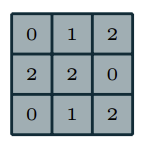
\includegraphics[width=0.1\textwidth]{imgs/cnnkernel.png}

\caption{ Ejemplo de filtro convolucional $(3,3)$. Fuente: \cite{cnn-arithmetic}}
\label{fig:cnnkernel}
\end{figure}

\begin{figure}[h!]

\centering
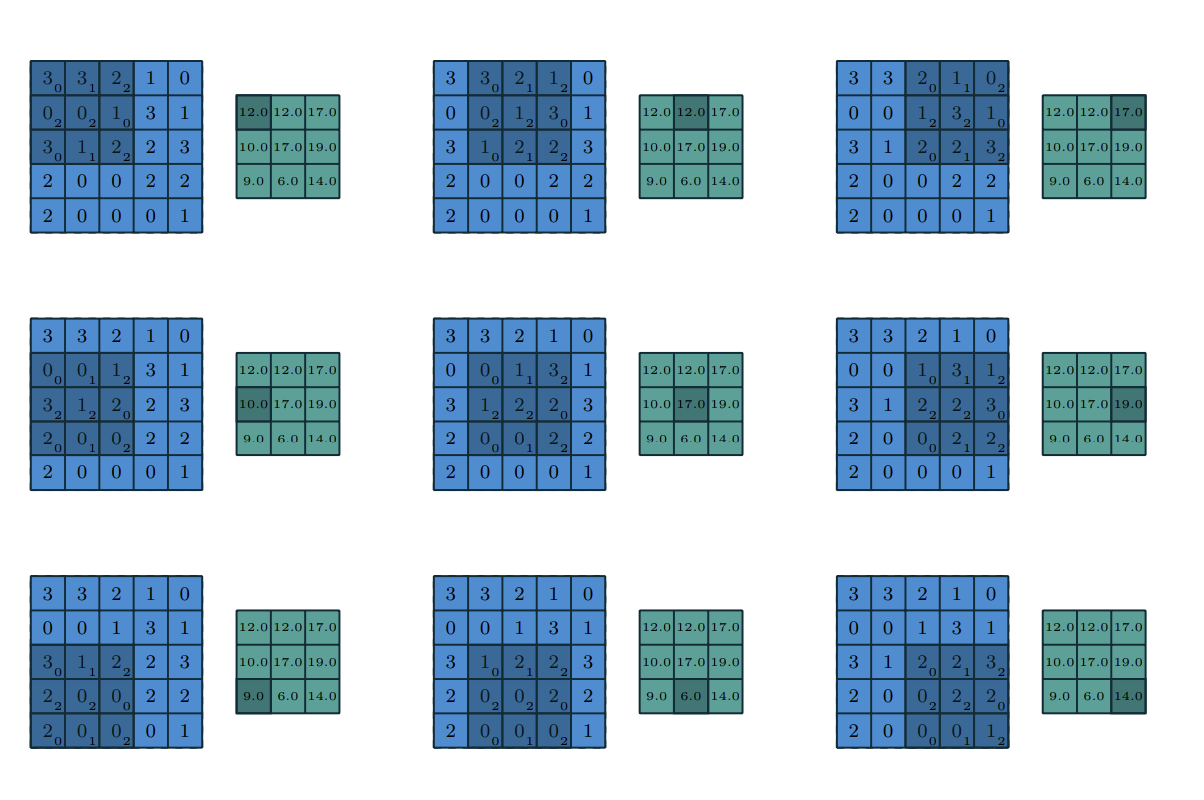
\includegraphics[width=1\textwidth]{imgs/cnnconv.png}

\caption{ El filtro de la imágen \ref{fig:cnnkernel} es aplicado a una matriz de entrada $(5,5)$ (color azul), produciendo una salida de $(3,3)$ (color aguamarina). Se han oscurecido respectivamente la zona rectangular de la matriz de entrada que interviene en la operación en cada paso, y la posición de la matriz de salida que constituye el resultado. Por razones de simplicidad hemos obviado el \textit{bias} $b$. Fuente: \cite{cnn-arithmetic}. }
\label{fig:cnnconv}
\end{figure}
Los valores de ponderación que determinan cómo se combinarán linealmente las entradas para formar las salidas son compartidos por cada salida con diferente $(W,H)$ (según \cite{lecun-invariance-shift}). La matriz $(w,h)$ con dichos valores se denomina \textit{\textbf{kernel}}. 

De tener múltiples canales de entrada ($C>1$), tendremos un filtro convolucional o \textit{kernel} para cada uno. A su vez, cada canal de  salida tiene un conjunto de filtros y \textit{bias} independiente. 

Las convoluciones ya se aplicaban en el procesamiento clásico de imágenes y eran llamadas también \textit{\textbf{filtros}}. Se usaban valores de \textit{kernels} que se sabían útiles para la extracción de ciertas características (como detección de bordes horizontales, diagonales o verticales). 

En el caso de las CNN, los \textit{filtros} serán entrenados, pretendiendo que se aprendan los valores que le resulten útiles. Además, la aplicación sucesiva de capas convolucionales apunta a que la componibilidad de los filtros sucesivos genere que la complejidad semántica de las características que se extraiga vaya en aumento con la profundidad.

\subsubsection{Aritmética de las convoluciones}

Para cada canal de la capa resultado se suman convoluciones distintas (con parámetros de \textit{kernel} distintos) de cada uno de los canales de la capa de entrada. 

Si tenemos una capa de entrada de tamaño $(W,H,c_{in})$ y le aplicamos un filtro de dimensión $(c_{out},c_{in},w,h)$ ($c_{in}$ canales de entrada, $c_{out}$ canales de salida y tamaño de kernel $w \times h$), se obtendrá una capa de salida de dimensión $(W-w+1, H-h+1, c_{out})$\footnote{Esto es considerando el caso de cero de \textit{padding} y uno de \textit{stride}. Conceptos que se explican en la subsección siguiente.}.  

Recordar que, además, tenemos un término de \textit{bias} por canal de salida ($c_{out}$ \textit{biases}, en este caso).

En el caso de las convoluciones, el número de parámetros de una capa sólo depende del tamaño del filtro: ($c_{out} \times c_{in} \times w \times h$) y el del \textit{bias}: $c_{out}$. A su vez, el número de computaciones sólo depende del producto entre el tamaño del filtro y el tamaño de la entrada. En el caso \textit{fully-connected}, tanto la cantidad de parámetros como el número de computaciones era del orden del producto de los tamaños de las activaciones sucesivas (debido a la matriz $W$). 

Esta reducción en el número de parámetros y el número de computaciones de cada capa permite entrenar modelos de muchas más capas.

Recordemos la fórmula para las capas densas (o \textit{fully-connected}) vista en la subsección \ref{subsection:nn-formulacion}:

\begin{equation*}
    f^j(\bar{h}^{j-1}) = \phi^j( {W^j}^\top \bar{h}^{j-1} + b^j)
\end{equation*}

La convolución es un caso particular de multiplicación de matrices, con restricciones sobre $W$.\footnote{Este hecho no debe sorprendernos ya que la convolución es una transformación lineal. Y las transformaciones lineales pueden ser expresadas como multiplicación de matrices.}

En la imagen \ref{fig:cnnmatmul1}.a se desgloza una convolución sobre una entrada de dimensión $(3,3)$ sobre la que se aplica un \textit{kernel} de $(2,2)$ produciendo una salida de $(2,2)$. Las combinaciones lineales dan lugar a las ecuaciones que se muestran en la figura \ref{fig:cnnmatmul1}.b. 
En la figura \ref{fig:cnnmatmul2} se muestra dicha operación como multiplicación de matrices. Notar que la matriz de la transformación (respectiva a $W$ de la fórmula vista anteriormente) posee ceros en determinadas entradas y los valores de ciertas entradas son compartidos, pueden variar según el entrenamiento pero deben ser iguales (ésto es  denominado en la jerga del Aprendizaje Profundo como \textit{shrared weights} o \textit{tied weights}).

\begin{figure}[h!]
\begin{subfigure}{0.45\textwidth}
\centering 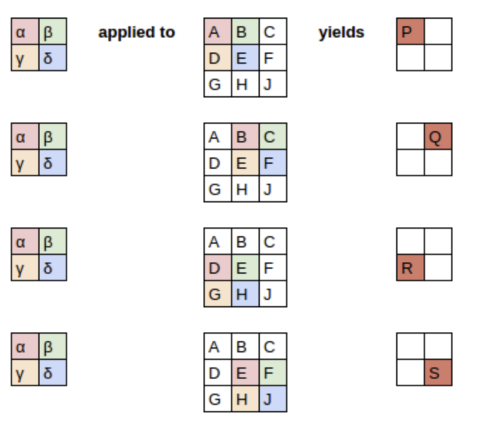
\includegraphics[width=0.5\textwidth]{imgs/cnndesgloce.png}
\end{subfigure}
\begin{subfigure}{0.45\textwidth}
\centering 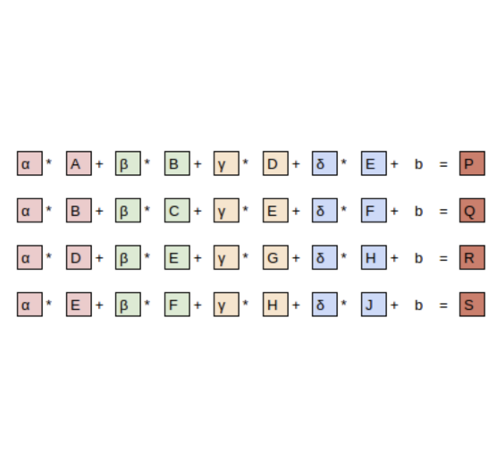
\includegraphics[width=0.5\textwidth]{imgs/cnndesgloceeqn.png}
\end{subfigure}
\caption{ A la izquierda el desgloce de la aplicación de un filtro convolucional. A la derecha las ecuaciones lineales que se desprenden de dicha convolución. El filtro está notado con las letras $\alpha$, $\beta$, $\gamma$ y $\delta$. La matriz de entrada corresponde a las letras de la $A$ a la $J$. La matriz de salida corresponde a las letras $P$, $Q$, $R$ y $S$. Fuente: \href{https://medium.com/impactai/cnns-from-different-viewpoints-fab7f52d159c}{\textit{``CNNs from different viewpoints''}}. Autor: Matthew Kleinsmith. }
\label{fig:cnnmatmul1}
\end{figure}

\begin{figure}[h!]

\centering
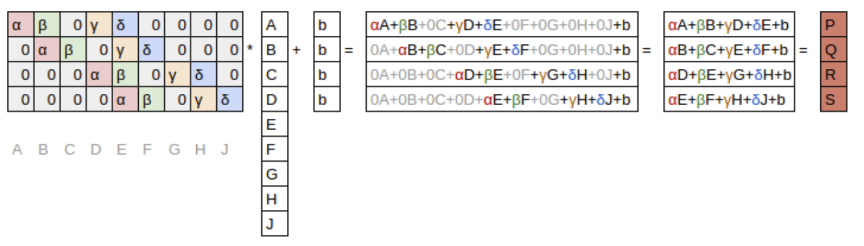
\includegraphics[width=0.85\textwidth]{imgs/cnnmatmul.png}

\caption{ Las ecuaciones de \ref{fig:cnnmatmul1}.b vistas como multiplicación de matrices. Fuente: \href{https://medium.com/impactai/cnns-from-different-viewpoints-fab7f52d159c}{\textit{``CNNs from different viewpoints''}}. Autor: Matthew Kleinsmith. }
\label{fig:cnnmatmul2}
\end{figure}

\paragraph{\textit{Padding} y \textit{Stride}}\mbox{}\\

El \textit{padding} y el \textit{stride} son hiperparámetros que configuran la convolución. Con la fórmula vista hasta ahora, el tamaño de la capa de salida está determinado por el de la entrada y el del \textit{kernel}. El propósito del \textit{padding} y el \textit{stride} es tener más flexibilidad a la hora de incidir en el tamaño de la salida.\\

El \textbf{\textit{padding}} consiste en agregar rellenos (generalmente 0) en los bordes de la capa de entrada.
Se agrega \textit{padding} para aumentar el tamaño de la salida.\\

Si pensamos a la aplicación de la convolución como un parche rectangular (el \textit{kernel}) que se va moviendo sobre la entrada (como una ventana deslizante), el \textbf{\textit{stride}} determina el tamaño del paso con el que avanza cada vez que se desplaza (ver figura \ref{fig:paddingstride}). Se agrega \textit{stride} para reducir el tamaño de la salida.

\begin{figure}[h!]

\centering
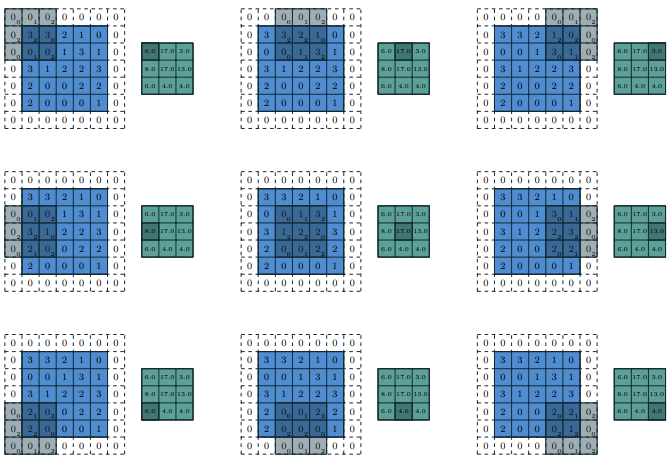
\includegraphics[width=1\textwidth]{imgs/convpadding.png}
\caption{ Ejemplo de aplicación de un \textit{kernel} convolucional de tamaño $(3,3)$ sobre una entrada de tamaño $(5,5)$ aplicando \textit{zero-padding} de $(1,1)$ y \textit{stride} de $(2,2)$. Fuente: \cite{cnn-arithmetic}}
\label{fig:paddingstride}
\end{figure}

Tanto el \textit{padding} como \textit{stride} pueden ser diferentes en el ancho o alto (aunque generalmente siempre se trabaja con cuadrados). 
En \cite{cnn-arithmetic} se muestra que si una dimensión de entrada posee tamaño $i$, y se aplica un \textit{kernel} de tamaño $k$, $p$ de \textit{padding} y $s$ de \textit{stride}, el tamaño $o$ de la salida obtenida es:

\begin{equation*}
    o = \ceil*{\frac{(i + 2p -k)}{s}} + 1
\end{equation*}

\paragraph{{\textit{Pooling}}}\mbox{}\\

Dada una entrada de tamaño $(W,H,C)$ las capas de \textit{pooling} la reducen a una capa de tamaño $(W',H',C)$ (con $W' < W$, $H' < H$), tomando el máximo (\textit{max-pooling}) o calculando el promedio (\textit{average-pooling}) de regiones rectangulares.

La reducción trabaja como una ``ventana deslizante'' que se va desplazando (al igual que el parche en la convolución) sobre la entrada. Ver figura \ref{fig:poolingexample}.

\begin{figure}[h!]
\centering
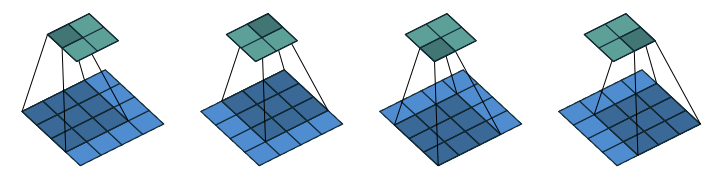
\includegraphics[width=0.85\textwidth]{imgs/convpooling.png}
\caption{ Las capas de \textit{pooling} se calculan con la misma lógica de ``ventana deslizante'' de las convoluciones. Fuente: \cite{cnn-arithmetic} }
\label{fig:poolingexample}
\end{figure}

Recomendamos \cite{cnn-arithmetic} para profundizar en el entendimiento de las convoluciones. Allí se explica y se esquematizan estos conceptos con puntillosidad.

\subsubsection{\textit{Receptive field}}

Se conoce como \textbf{área de recepción} (\textit{receptive field}) al área de la imagen original que incide sobre el cálculo de cierta activación. En \cite{fastbook} se muestra el esquema presentado en la figura \ref{fig:receptive-fields}, donde se puede ver cómo a medida que aumenta la profundidad el \textit{receptive field} es más grande. O sea que una gran porción de la imágen interviene en el cálculo de cada activación (característica) de las capas profundas. Es de esperar entonces que al aumentar la profundidad, será necesario aumentar la cantidad de filtros (canales), porque la sección de la entrada correspondiente que es representada en cada posición $(w,h)$ de la activación, es de dimensionalidad mayor. Y por ende se necesitará, probablemente, más \textit{features} para describirla.

Como se verá en el apartado \ref{subsubsection:visualizing}, las activaciones de capas más profundas corresponden a características semánticamente más complejas. Es de esperar también, que sean necesarios más filtros en las capas más profundas ya que el número de características semánticamente complejas probablemente sea mayor que el de características más simples.

\begin{figure}[h!]
\centering
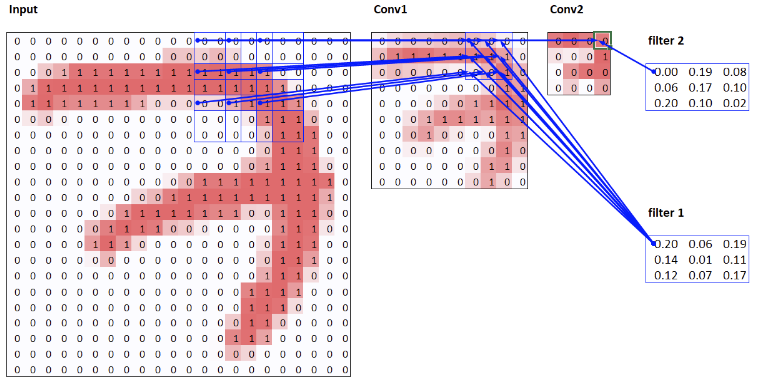
\includegraphics[width=1\textwidth]{imgs/convreceptive.png}
\caption{ En \cite{fastbook} se implementan dos capas de convoluciones en planillas de cálculo, con el fin de visualizar como el procesamiento se aplica sobre la capa de entrada (\textit{Input}) obteniendo sucesivamente las activaciones de cada convolución (\textit{Conv1} y \textit{Conv2}). \\ También se muestra la zona respectiva de la imágen para cada elemento de la salida (en azul, el \textit{receptive field}) y su relación con los filtros. \\ Fuente \cite{fastbook}. }
\label{fig:receptive-fields}
\end{figure}

A su vez en las primeras capas, el tamaño de la capa de entrada es grande, por lo que utilizar pocos filtros para ellas reducirá considerablemente el número de computaciones (que, como se dijo, es del orden del producto entre el tamaño de la capa de entrada y el tamaño del filtro).

\subsubsection{Visualizando las características aprendidas} \label{subsubsection:visualizing}

Las características aprendidas capa por capa fueron estudiadas por \cite{visualizecnn} para el modelo de cinco capas \textit{AlexNet} que ganó la competencia de \textit{ImageNet} 2012 \cite{alexnet}. Se graficó para cada capa, la intensidad de los pesos de los filtros y las partes respectivas de la imágenes (\textit{receptive fields}) para las cuáles los filtros mostraban una mayor activación (ver figura \ref{fig:visualizecnn}). 

Se observa cómo las primeras capas aprenden a reconocer características básicas (diagonales, horizontales y verticales de ciertos colores), las capas intermedias características más complejas (espirales, curvas y diferentes texturas), hasta las últimas capas que aprenden a extraer conceptos semánticos de alto nivel (flores, perros, personas, vehículos, etc).

Muchas de las características aprendidas por el modelo son parecidas a las que se solían extraer manualmente por algoritmos anteriores de análisis de imágenes. 

El trabajo nos muestra no solamente una forma de ``visualizar qué aprenden los filtros'' en las \textit{CNN}, sino también prueba el hecho de que las representaciones aprendidas son patrones deseables, componibles y de creciente complejidad.

\begin{figure}[h!]

\centering
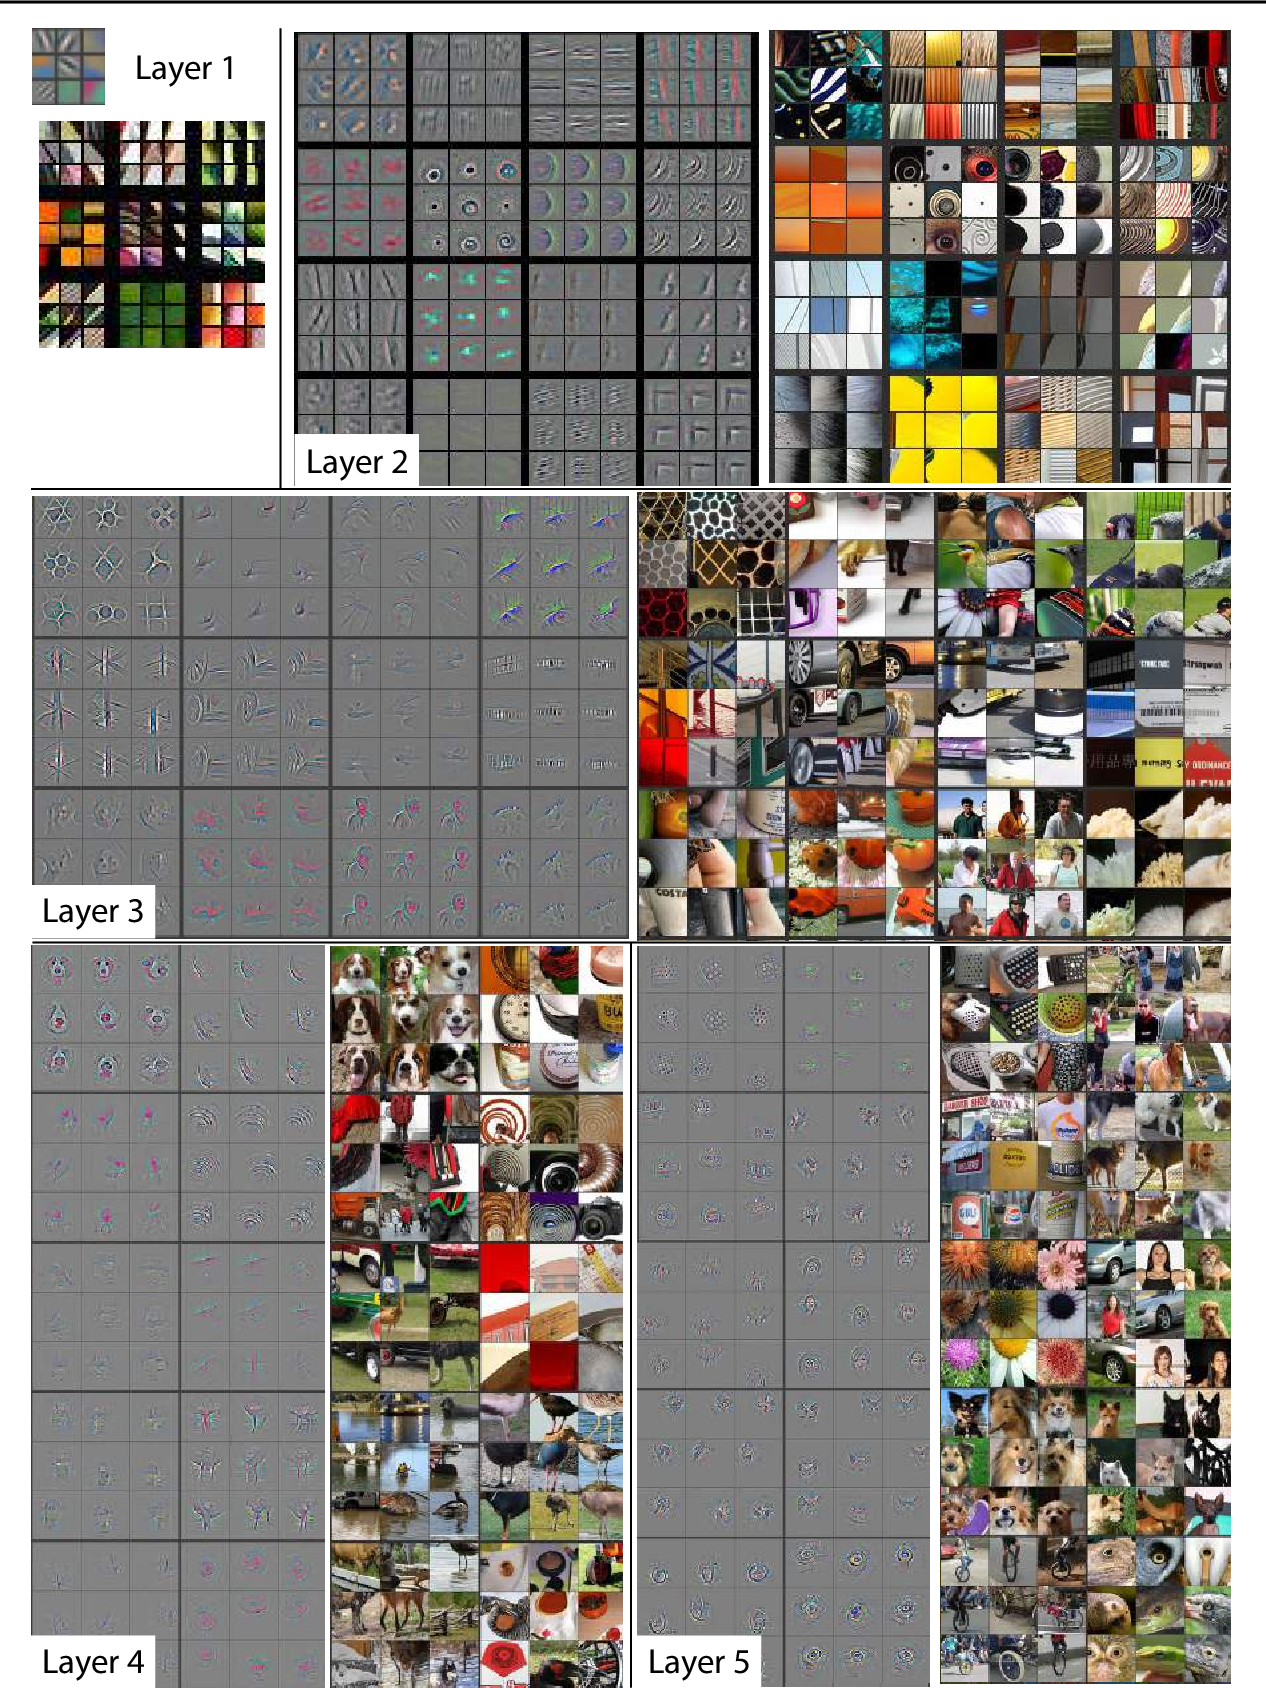
\includegraphics[width=0.98\textwidth]{imgs/visualizecnn.png}

\caption{ En gris, el valor de los filtros convolucionales. En colores, los parches de \textit{receptive field} que más activaron a los filtros respectivos. Fuente: \cite{visualizecnn}}
\label{fig:visualizecnn}
\end{figure}

\subsubsection{Redes completamente convolucionales}

Una diferencia entre las capas convolucionales y las densas (\textit{fully-connected}) está en cómo se relaciona el tamaño de la capa de entrada, el tamaño del \textit{kernel} (los parámetros) y el tamaño de la capa de salida.

Para una convolución dada, el tamaño de la entrada no depende de la misma (puede aplicarse a diferentes tamaños de entrada). Pero fijada la convolución, el tamaño de la salida será función de la entrada.

En el caso de las capas densas, dada una capa (dado $W$ y $b$), el tamaño de la entrada y la salida está completamente determinado: sólo puede aplicarse a entradas de un único tamaño, produciendo salidas de un tamaño también determinado. \\

A la hora de diseñar arquitecturas de Redes Neuronales siempre se debe pensar cómo se transforma la entrada (de cierto tamaño) en la salida (del tamaño de la predicción deseada).

Arquitecturas como \textit{VGG} (ganadora de \textit{ImageNet 2013} \cite{vgg}) apilan cierto número de convoluciones (como se dijo, con número de filtros creciente) para luego aplanar las características y aplicar una sucesión de capas densas sobre las mismas. Ésto hace que, si bien las convoluciones iniciales pueden ser aplicadas a imágenes de cualquier tamaño, la entrada de las capas densas deba ser (como se dijo) fijo. Y por ende el tamaño de la entrada original también deba ser fijo.

Una manera de evitar esta dependencia respecto del tamaño de la entrada $(W,H,C)$, consiste en apilar tantas capas de \textit{stride} (o \textit{pooling}) como sean necesarias para reducir el tamaño de la salida convolucional a $(1,1,C')$ y luego aplicar capas densas para obtener la predicción del tamaño deseado $c_{out}$. De este modo el tamaño de las capas densas sólo dependerá de $C'$, y en última instancia del número de canales de la entrada $C$, pero será independiente de $W$ y $H$.  Pero nuevamente, esto es sólo posible si conocemos el tamaño de la entrada de antemano (de lo contrario no sabríamos \textit{cuántas} capas convolucionales con \textit{stride} aplicar).\\

La solución ha sido transformar la salida de la pila de convoluciones de tamaño $(W',H',C')$ haciendo un \textit{Pooling Adaptativo},\footnote{Éstos, en vez de poseer un tamaño de ventana fijo, tienen un tamaño de salida fijo y utilizan para ello la ventana necesaria.} lo cuál escencialmente acumulará para cada canal todos los valores de las activaciones (a lo alto y ancho de la última activación), de modo de obtener una salida de tamaño $(1,1,C')$. Así, la arquitectura se mantiene totalmente desacoplada del tamaño de entrada, ya que la capa de \textit{pooling} funciona para cualquier $(W',H')$ porque es simplemente acumular los valores de cada canal usando cierta operación. 

Éstas redes se denominan \textbf{Redes Completamente Convolucionales} (\textit{FCN}, en inglés \textit{Fully Convolutional Network}). 

Luego la salida de dimensión $C'$ puede ser llevado a la predicción $c_{out}$ utilizando capas densas. Notar que $C'$ no varía si se utilizan entradas de diferente ancho o alto, ya que los canales son independientes de $W$ y $H$. Sólo depende de la cantidad de canales de entrada $C$. 

La primera parte de la arquitectura (hasta la salida de dimensión $C'$) es denominada cuerpo (\textbf{\textit{body}}). Y la segunda parte (capas densas) es llamada cabeza (\textbf{\textit{head}}). 

Estas redes pueden ser entrenadas para imágenes de cierto tamaño y usadas en imágenes de otro tamaño (notar que la cantidad de canales de la entrada debe ser el mismo).

\textbf{Nota:} la última capa del \textit{body} combina los filtros independientemente de su posición. Es importante que el dominio donde se aplique sea válido la hipótesis de \textit{invariancia traslacional}.

\subsubsection{\textit{ResNets}}

En 2015 los autores de \cite{resnet} observaron, trabajando con las ya presentadas redes \textit{VGG}, que al agregar más capas convolucionales obtenían peores valores del error y la causa no era el sobreajuste, puesto que lo mismo sucedía durante el entrenamiento (ver \ref{fig:convresnetidea}).

\begin{figure}[h!]
\centering
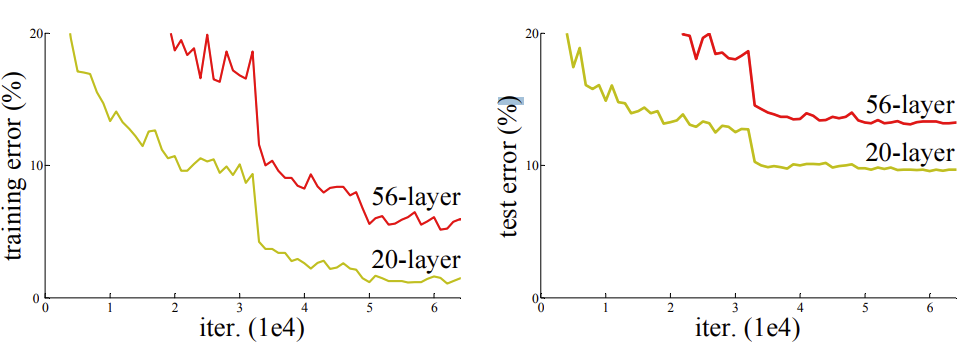
\includegraphics[width=0.85\textwidth]{imgs/convresnetidea.png}
\caption{ Observación clave que condujo al desarrollo de redes residuales. Fuente: \cite{resnet} }
\label{fig:convresnetidea}
\end{figure}

Tampoco se debía a que el cambio de arquitectura restringiera el espacio de hipótesis puesto que las capas innecesarias bien podrían aprender la identidad ($W = I$ y $b = \overline{0}$). Pero esto no sucedía: por alguna razón el algoritmo de optimización no encontraba esta solución.

Luego reemplazaron la capa de convolución:

\begin{equation*}
y = conv(x)    
\end{equation*}

Por la siguiente formulación:

\begin{equation*}
y = conv(x) + x
\end{equation*}

Además, inicializaron el parámetro $\gamma$ (de \textit{batch normalization}) en $0$. De modo que el entrenamiento podía variarlo pero inicialmente la capa era en sí la identidad. Ésta idea dio lugar al bloque que denominaron \textit{skip-connection} (ver esquema \ref{fig:convskipconn}).

\begin{figure}[h!]
\centering
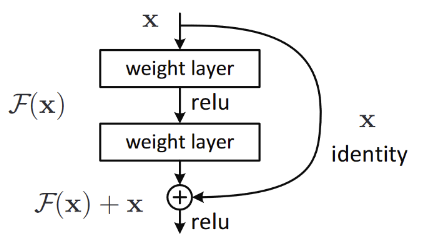
\includegraphics[width=0.5\textwidth]{imgs/convskipconn.png}
\caption{ El bloque usado en \cite{resnet} usa dos convoluciones sucesivas. La idea básica es la misma que se ha explicado: las convoluciones ahora deben aprender el \textit{residuo} de la función objetivo (menos la identidad). De modo que aprender la identidad resulta trivial. Fuente: \cite{resnet} }
\label{fig:convskipconn}
\end{figure}

En este bloque se basa la familia de \textit{Residual Neural Network} (\textit{ResNets}) ganadoras de la competencia ImageNet 2015 (\textit{error rate} $3.57 \%$), acabando con la dominancia de las \textit{VGG}. \cite{resnet}

El estudio posterior ha constatado la superioridad de estas arquitecturas. En \cite{visualizing-landscapes} se muestra que el uso de \textit{skip-connections}{ genera funciones de costo más suaves, con menos mínimos empinados (ver figura \ref{fig:visualresnetloss}) y por ende contribuyen a una mejor generalización.

\begin{figure}[h!]
\centering
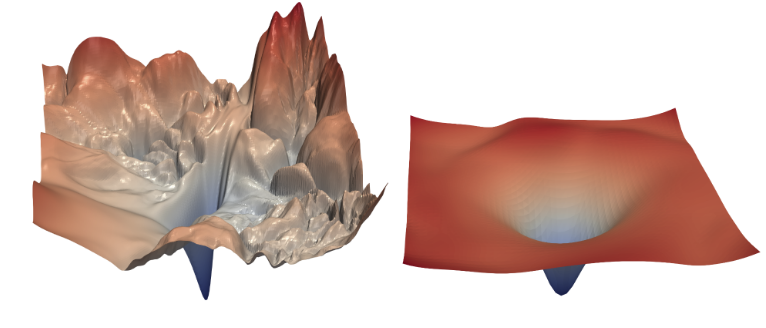
\includegraphics[width=0.85\textwidth]{imgs/convresnetsurface.png}
\caption{ Por medio de métodos de visualización lograron una representación bidimensional de la función de costo. A la derecha se ve como resulta la superficie de costo al utilizar \textit{skip-connections} Fuente: \cite{visualizing-landscapes} }
\label{fig:visualresnetloss}
\end{figure}

En \cite{cnntricks} se estudian algunos ajustes que perfeccionan la arquitectura de las \textit{ResNets}. En el trabajo se utilizan estos ajustes (incorporados a la librería FastAI). Por ejemplo se utilizan simples convoluciones en las primeras capas para mantenerlas más simples (ya que como se dijo son computacionalmente de mayor costo porque aplican a una entrada más grande). Y se reemplazan las \textit{skip-connections} por \textit{Bottlneck Layers} (ver esquema \ref{fig:bottleneck}) que son más rápidos permitiendo agregar más filtros.

\begin{figure}[h!]
\centering
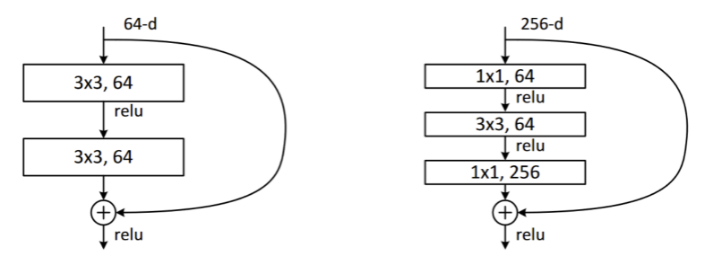
\includegraphics[width=0.8\textwidth]{imgs/convbottleneck.png}
\caption{ \cite{cnntricks} reemplaza las \textit{skip-connections} (izquierda) por \textit{Bottlneck Layers} (derecha) Fuente: \cite{cnntricks} }
\label{fig:bottleneck}
\end{figure}

\subsubsection{\textit{Fine-tuning}}

El hecho de que las características aprendidas sean patrones deseables y componibles (como se vio en el apartado \ref{subsubsection:visualizing}) da apoyo teórico a que puedan ser reutilizadas, entre problemas similares.

Se conoce como \textbf{\textit{fine-tunning}} a la técnica de transferencia del aprendizaje (\textit{transfer learning}) donde los parámetros son entrenados partiendo de la base de un modelo que ya ha sido entrenado para un conjunto de datos diferente (e incluso para un problema diferente) al que se quiere resolver.

Así, por ejemplo, si se quiere hacer un clasificador de fotografías de tipos de automóviles, se pueden obtener resultados con precisión del estado del arte aún sin contar con demasiados datos, y entrenando unas pocas épocas, si re-entrenamos un modelo ya entrando sobre el \textit{dataset ImageNet} (por ejemplo podríamos usar \textit{ResNet-50}). La técnica incluso sirve para problemas diferentes a la clasificación (por más que el problema original de \textit{ImageNet} es entrenar un clasificador), ya que lo transferible son las  de características extraídas en las capas intermedias. Por ejemplo se pueden entrenar modelos para problemas de regresión, \textit{tagging} multi-clase, etc.\\

En general cuando se aplica \textit{fine-tunning} se conserva la parte de la arquitectura que hemos denominado \textit{body} y se coloca un nuevo \textit{head}. Ésto es debido a que el \textit{head} es problema-específico, ya que depende del tamaño de la salida $c_{out}$. Además, las características codificadas por las últimas capas tendrán que ver con las cuestiones específicas del problema y lo que se quiere transferir son las representaciones que son trasladables entre los dos problemas.

La librería \textit{FastAI} posee la funcionalidad de fácilmente congelar los pesos del \textit{body}, de modo de entrenar unas épocas modificando el \textit{head} solamente (ya que al ser inicializado de cero, contendrá pesos aleatorios). Esto tiene sentido ya que no queremos que la señal de \textit{backpropagation} de un \textit{head} totalmente aleatorio arruine las representaciones útiles que intentamos transferir. Además el congelamiento de las primeras capas reduce el problema de \textit{internal covariance shift}, ya que sólo varía el \textit{head} y no las capas anteriores (su entrada). Hay quienes incluso pre-computan las activaciones de salida del \textit{body}, ya que no variarán durante esta fase, para no volverlas a calcular. Luego podemos descongelar los parámetros del \textit{body} y entrenar todo el modelo en su conjunto. \cite{fastbook}

En línea con el argumento del párrafo anterior \cite{discriminative-lr}\footnote{Jason Yosinski et al. desarrolló este método originalmente para el problema de NLP ULMFiT. Cómo muchos conceptos de Aprendizaje Profundo, es extrapolable a otras áreas.} propone asignar \textit{learning rates} diferenciados durante el proceso de \textit{fine tunning} de modo que las primeras capas (más cercanas a la entrada) no varíen tanto como las últimas. Ésto está en consonancia con el hecho de que las representaciones de las primeras capas son conceptos más simples y serán más extrapolables, en cambio las capas posteriores (incluso del \textit{body}) son más complejos y tendrán que re-adaptarse al problema específico.


\subsection{Arquitecturas de redes siamesas} \label{subsection:siamesas}

Como se discutió en el capítulo \ref{chapter:trabajos-anteriores}, muchos problemas de similitud de imágenes (por ejemplo \textit{Face Verification} o similitud de firmas) no se resuelven entrenando un clasificador con una clase por identidad, sino aprendiendo una \textit{representación} y una \textit{métrica} que permitan comparar pares de ejemplos. Las \textbf{redes siamesas} constituyen una arquitectura estándar para este tipo de problemas \cite{siamess-lecun}. La idea central es utilizar un mismo \textit{encoder} convolucional $G_W$ para mapear cada imagen $img$ a un vector de características de dimensión fija (un \textit{embedding}):
\begin{equation*}
    z = G_W(img) \in \mathbb{R}^d,
\end{equation*}
compartiendo los pesos $W$ entre ambas ramas de la red (lo que en la jerga se conoce como \textit{tied weights}). 

A partir de estos \textit{embeddings} se define una función de distancia $d(z_1, z_2)$ (por ejemplo la distancia euclídea o la distancia coseno) y se entrena el modelo para que firmas (o imágenes) de la misma clase queden “cerca” en el espacio de representación, y las de clases distintas “lejos”. Desde esta perspectiva, el clasificador binario que decide si dos firmas son de la misma autoría o no pasa a ser un umbral sobre la distancia:
\begin{equation*}
    autoresNoCoinciden(img_1, img_2) = 
    \left\{
        \begin{array}{ll}
        \text{Verdadero} & \text{si } d(G_W(img_1), G_W(img_2)) > \tau \\
        \text{Falso}     & \text{si } d(G_W(img_1), G_W(img_2)) \leq \tau
        \end{array}
    \right.
\end{equation*}
para algún umbral $\tau$ elegido según los criterios de costo–beneficio discutidos en \ref{subsubsection:costo-beneficio}. En nuestro caso particular, este esquema permite aprovechar el mismo \textit{encoder} convolucional para firmar autores nunca vistos durante el entrenamiento, algo que sería muy difícil de lograr con un clasificador “uno contra todos” por autor.

\subsubsection{Triplet loss} \label{subsubsection:triplet-loss}

Una forma efectiva de entrenar redes siamesas es mediante funciones de costo diseñadas específicamente para \textit{aprendizaje de métricas}. Entre ellas, una de las más utilizadas es la \textbf{\textit{triplet loss}}. En lugar de trabajar con pares $(img_1, img_2)$, se consideran tripletas $(a, p, n)$:
\begin{itemize}
    \item $a$ (\textit{anchor}): una firma de referencia.
    \item $p$ (\textit{positive}): una firma del mismo autor que $a$.
    \item $n$ (\textit{negative}): una firma de un autor distinto.
\end{itemize}

Sea $z_a = G_W(a)$, $z_p = G_W(p)$ y $z_n = G_W(n)$ sus \textit{embeddings}. La triplet loss impone que la distancia entre el ancla y el positivo sea menor, al menos por un margen $\alpha > 0$, que la distancia entre el ancla y el negativo:
\begin{equation*}
    L(a,p,n) = \max\big(0,\ d(z_a, z_p) - d(z_a, z_n) + \alpha \big).
\end{equation*}
Intuitivamente, el costo es cero siempre que $z_a$ esté "más cerca" de $z_p$ que de $z_n$ por al menos $\alpha$, y positivo en caso contrario. El entrenamiento busca minimizar la suma (o el promedio) de $L(a,p,n)$ sobre un conjunto de tripletas construidas a partir del \textit{dataset}. 

Cabe notar que esta formulación resulta menos restrictiva que otras funciones de costo que fuerzan a los ejemplos de una misma clase a colapsar en un único punto del espacio de representación. La triplet loss únicamente exige que los ejemplos positivos estén más cerca del ancla que los negativos, permitiendo así que las muestras de un mismo autor mantengan cierta dispersión entre sí. Esta flexibilidad es deseable en dominios como el de firmas manuscritas, donde existe variabilidad intra-clase natural y no resulta razonable pretender que todas las instancias de un autor converjan a una representación idéntica.

En la práctica es crucial la estrategia con la que se generan dichas tripletas: si se eligen tripletas “fáciles” (para las cuales la desigualdad ya se cumple ampliamente), el gradiente será casi nulo y el modelo aprenderá poco; por el contrario, seleccionar tripletas demasiado difíciles puede llevar a inestabilidades numéricas o a un entrenamiento que no converge. Existen esquemas \textit{offline} (las tripletas se pre–generan) y \textit{online} (se seleccionan dinámicamente tripletas informativas dentro de cada \textit{mini-batch}), que se describen con más detalle en el capítulo de Experimentos. En nuestro trabajo utilizamos variantes de \textit{triplet loss} precisamente para forzar que firmas de la misma autoría colapsen en regiones compactas del espacio de representación y que firmas de diferentes autores queden claramente separadas, lo que se traduce luego en mejores métricas de \textit{precision} y \textit{recall} en el problema binario definido en \ref{section:objectives}.




\chapter{Formulación del problema} \label{formulacion-del-problema}

AGREGAR LA FALTA DE FIRMAS!!

En el presente capítulo se formula la problemática a resolver y se eligen las métricas de satisfactibilidad.

En el capítulo \ref{chapter:trabajos-anteriores} hacemos un sondeo de soluciones a problemas similares e introducimos los conjuntos de datos que luego utilizaremos en nuestros experimentos.

La metodología para llegar a los resultados y el detalle de los mismos se encuentran en el capítulo \ref{chapter:experimentos}.

\section{Preliminares}

El trabajo se enmarca en el proyecto de incorporación de dispositivos tecnológicos que asistan el proceso electoral impulsado por el Gobierno de Santa Fe a través de las Secretarías de Tecnologías para la Gestión. Y más especificamente, del sistema de escrutinio provisorio con asistencia digital\footnote{En \cite{unr1} podemos encontrar una detallada descripción del Proceso de Escrutinio Provisorio Asistido Digitalmente. En \cite{qrs} se encuentran las especificaciones técnicas de los \textit{QRs} utilizados para la verificación de consistencia de los datos registrados en los telegramas.}.

Actualmente el Sistema de Escaneo y Transmisión de Telegramas (\textit{SETT}) y Sistema de Asistencia a las Autoridades de Mesa (\textit{SIAAM}) proveen soluciones robustas de asistencia digital al proceso de escrutinio provisorio demostrando (véase \cite{unr-informe}):
\begin{enumerate}
    \item Aumentar el cubrimiento de mesas en el escrutinio provisional.
    \item Disminuir el porcentaje de votos ``a determinar en el escrutinio definitivo''.
    \item Aumentar considerablemente la celeridad en la carga de telegramas.
    \item  Disminuir las solicitudes de re-confección de telegramas.
\end{enumerate}

\section{Sobre los telegramas de votación en Santa Fe}

Hoy por hoy se detecta cuando el telegrama está en el centro de cómputo. Si el sistema de escaneo contara con un detector de firmas y similaridad se podrían reconocer antes y sería probable que se arreglar.


En las elecciones provinciales de Santa Fe, cada mesa de votación realiza un recuento de las actas emitidas en las mismas y se confeccionan telegramas con un formato específico con los resultados. Los mismos consisten en una tabla con la cantidad de votos para cada partido y cargo a elegir. Se puede ver un ejemplo en la figura \ref{fig:telegramas}.

El telegrama debe ser firmado por las autoridades (presidente y auxiliares) y los fiscales de la mesa respectiva. De poseer varias páginas la firma debe estar en todas y coincidir. En la figura \ref{fig:telegramas-firmas}  se puede ver el recorte de la sección de firmas, de dos páginas distintas que pertenecen a un mismo telegrama.

\begin{figure}[h!]

\begin{subfigure}{0.45\textwidth}
\begin{center}
    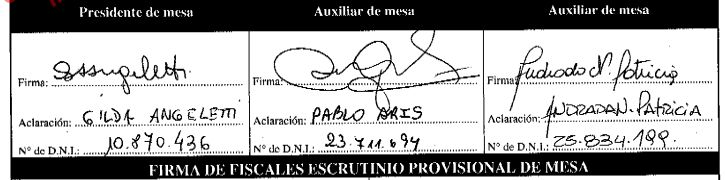
\includegraphics[width=0.75\textwidth]{imgs/telegramas2.png}
\end{center}
\end{subfigure}

\begin{subfigure}{0.45\textwidth}
\begin{center}
    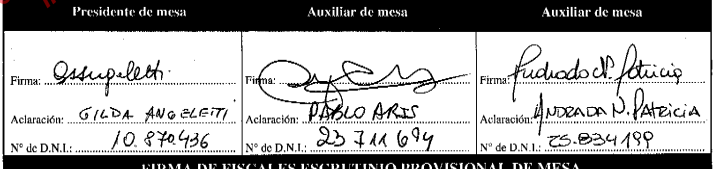
\includegraphics[width=0.75\textwidth]{imgs/telegramas3.png}
\end{center}
\end{subfigure}

\caption{ Recorte de la sección de firmas de dos páginas de un mismo telegrama. Para ver un telegrama completo ir al a figura \ref{fig:telegramas}. En las secciones donde aparecen firmas también aparecen otros trazos del formulario como la línea de puntos. Fuente: }
\label{fig:telegramas-firmas}
\end{figure}

\begin{figure}[h!]

\begin{subfigure}{0.45\textwidth}
\begin{center}
 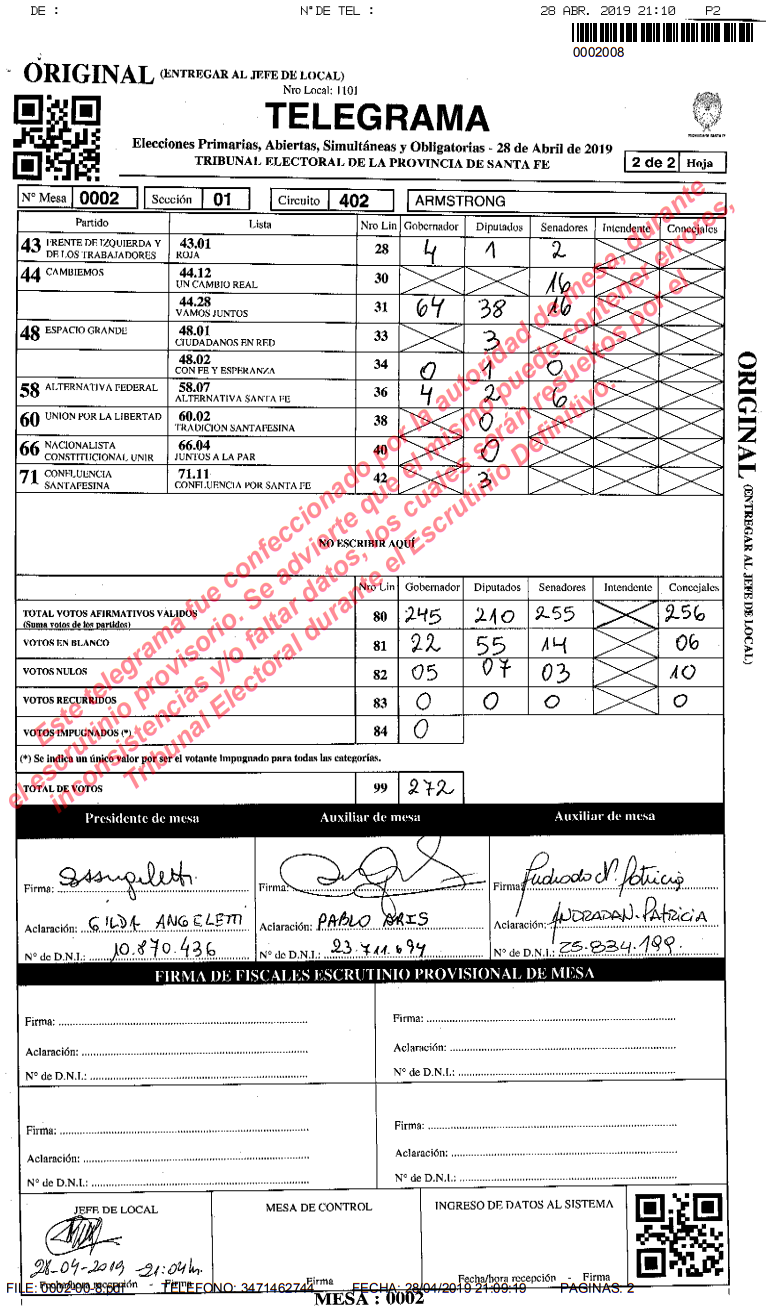
\includegraphics[width=0.85\textwidth]{imgs/telegramas1.png}
 \end{center}
\end{subfigure}

\caption{ Ejemplo de un telegrama electoral de las elecciones primarias de 2019. El formato es conocido meses antes de las elecciones. Los códigos QR de las esquinas sirven para enderezar las fotografías de los telegramas. Fuente: \cite{unr1} }
\label{fig:telegramas}
\end{figure}


Luego los telegramas son transmitidos al centro de cómputo del escrutinio provisorio. Operadores humanos llevan la labor de carga de datos, realizándose chequeos de consistencia. Si se detectan errores en esta fase puede pedírsele a las autoridades de la mesa que realicen nuevamente la confección del telegrama y/o  el recuento según sea necesario. Nos referiremos a estos eventos como \textbf{retransmisiones}. Las autoridades de mesa deben esperar la confirmación del centro de cómputo de que el telegrama ha sido chequeado y cargado para considerar su labor finalizada.


Según surge de las estadísticas del informe \cite{unr-informe} (sección 7.3), de poderse automatizar los procesos de:
\begin{enumerate}
    \item Detectar que firmas de las autoridades de mesa estén presentes y coincidan en todas las páginas de un mismo telegrama.
    \item Detectar los números en grillas de telegramas de votación (y hacer chequeos de consistencia, como por ejemplo verificación de totales).
\end{enumerate}
Se podrían introducir chequeos automáticos antes de que el telegrama sea enviado al centro de cómputo logrando:
\begin{itemize}
    \item  Aumentar la celeridad en la carga de telegramas en el centro de cómputo.
    \item Disminuir las solicitudes de reenvío de telegramas.
\end{itemize}
En definitiva, disminuir en gran medida el trabajo humano.\\

Nos enfoquermoes en el primer problema: reconocer firmas y constatar coincidencia entre ellas.

\section{Definiendo los objetivos}
\label{section:objectives}

Como veremos en el capítulo \ref{chapter:trabajos-anteriores}, existen variedad de problemas similares relativos a firmas manuscritas.

Como el diseño de los telegramas se conoce de antemano, y las firmas que se quieren analizar aparecen en posiciones determinadas de la página, no es necesario resolver el problema general de \textit{Signature Recognition}. Nos bastará recortar dicha sección de la página y determinar si hay o no una firma. Esto, hasta hace muy poco tiempo atrás consistía en un problema para nada trivial, sobretodo puesto que en la sección aparecen otros trazos como partes del formulario. No obstante, con el estado actual de los analizadores de imágenes hemos podido resolverlo sin demasiado ajetreo y hemos extendido y focalizado el trabajo de la tesina en el problema -mucho más desafiante- de similitud de firmas.\\

El problema de determinar si dos firmas son el mismo \textit{tipo de firmas} (fueron realizadas por el mismo autor) puede expresarse más formalmente como el predicado\footnote{En nuestro caso contamos con imágenes de las firmas manuscritas, pero existen otros ámbitos donde se cuenta también con información dinámica (temporal) acerca de cómo fue generado el trazo. También existen conjuntos de datos para este otro problema.}:
\begin{equation*}
    autoresCoinciden( firmaA : Imagen, firmaB : Imagen) \rightarrow Bool
\end{equation*}
Es así que el problema puede ser tratado como un problema de clasificación binaria donde las imágenes de ambas firmas constituyen la entrada.\\

Además, como se detalló en el apartado \ref{subsubsection:metricbinary}, al querer detectar \textit{no coincidencias} (ya que las mismas constituyen un error en la confección del telegrama analizado), trateremos a las mismas como clase positiva. Así nuestro clasificador tratará de computar la siguiente función:

\begin{equation*}
    autoresNoCoinciden( firmaA : Imagen, firmaB : Imagen) \rightarrow Bool
\end{equation*}

\subsection{Modelado del problema}

A diferencia del problema de \textit{signature verification} donde hay que determinar si una firma pertenece al autor que declara ser (conociendo previamente ciertas firmas para cada autor), en nuestro problema es posible (y probable) que las firmas sobre las que aplicaremos nuestra solución sean de autores completamente distintos a los que usamos para entrenar. Es por ello que no podemos entrenar un clasificador binario para cada autor como se hace en algunos trabajos relacionados.

Nuestra entrada serán pares de firmas y nuestra salida un booleano que indicará si es clasificado como coincidencia o no. Formalmente, una solución al problema consiste en un par de funciones:
\begin{itemize}
    \item $fit(firmas, clases)$: entrena la solución utilizando un conjunto de imágenes para las cuales se conocen sus respectivos autores.
    \item $predict(img_1, img_2) \rightarrow Bool$: determina si dos firmas son una coincidencia o no.
\end{itemize}

\subsection{Definición de los experimentos}
\label{subsection:definicion-experimentos}

Cada experimento consiste en una 3-upla $(dev, test, test\_ds)$:
\begin{itemize}
    \item \textbf{dev} y \textbf{test}: son duplas $(firmas, clases)$ con paths hacia imágenes y sus clases (autores) respectivamente. Los elementos de $dev$ se utilizan para entrenar.
    \item \textbf{test\_ds}: consiste en 3-uplas $(idx_1, idx_2, bool)$ donde el booleano determina si $test[idx_1]$ y $test[idx_2]$ constituyen un matcheo o no. Es importante usar las mismas 3-uplas para evaluar cada solución de modo que la comparación sea correcta.
\end{itemize}

\subsubsection{Desarrollo: entrenamiento y validación}

Del conjunto de firmas dedicadas al desarrollo ($dev$) se obtienen tanto los subconjuntos de entrenamiento (para encontrar los parámetros del modelo) como de validación (para encontrar los hiperparámetros).

La cantidad de clases (autores) distintas en el conjunto de desarrollo puede ser escasa. En dichos casos las métricas en validación pueden variar demasiado dependiendo de la elección de partición entrenamiento/validación, lo cual hace sensible a la elección de hiperparámetros. Es por eso que utilizamos un \textbf{5-fold cross validation} sobre el conjunto de desarrollo para generar 5 particiones, de modo que la elección de hiperparámetros sea más robusta.

Es importante, si vamos a comparar el score de validación de varios modelos, fijar también los emparejamientos de elementos (recordemos que nuestra solución toma pares) para los subconjuntos de validación.

\subsubsection{Construcción del conjunto de pares}

Al armar las parejas en los conjuntos de test y validación se construyen siempre conjuntos balanceados: hay tantas coincidencias como no coincidencias. Si se generaran todas las parejas posibles el conjunto contendría muchas más no coincidencias que coincidencias.

Para generar coincidencias, para cada clase se arman parejas sin repetirlas (sin considerar orden). Un parámetro $cls\_sampling\_limit$ limita la cantidad de veces que un elemento aparece en las parejas auténticas. Para generar pares no coincidentes se toma para cada elemento otros elementos no coincidentes (tantos como coincidentes) dejando el conjunto balanceado.

\subsection{Elección de la métrica}

El objetivo de los modelos es realizar una predicción lo más acertada posible. En la práctica, las predicciones se usan para tomar decisiones. Es así que los diferentes tipos de error no son equiparables. Como se vio en \ref{subsubsection:metricbinary} en el caso de la clasificación binaria tenemos \textit{falsos negativos} y \textit{falsos positivos}. \\

En nuestro caso, al aceptar pares de firmas que no coinciden (falsos negativos), el automatismo no cumplirá su objetivo de disminuir las retransmisiones y el trabajo humano innecesario. En caso de falsos positivos, las alarmas emitidas por el asistente serán incorrectas corriendo el riesgo de que el usuario desestime su opinión y que lejos de aumentar la eficiencia del proceso entorpezca la labor. \\

Es por esto que es importante no basarse en la tasa de aciertos (\textit{accuracy}), sino medir ambos errores de forma separada. Esto también es necesario cuando se trabaja con conjuntos de datos desbalanceados.\\

Para nuestro trabajo tomaremos como métrica a maximizar: ``la mayor \textit{precision} para la cuál el \textit{recall} sea mayor que 0.9''. Así, nuestra métrica tendrá un significado práctico: queremos que nuestro sistema capture el 90\% de los errores de firmas no coincidentes (reduciendo al 10\% el número de retransmisiones por esta causa) y que sea lo más fiable posible (en el sentido de que no genere falsas alarmas).

Habiendo calculado esta métrica, podría ser útil dar a conocer al usuario el umbral de \textit{precision}. Esto de alguna manera le indicará el ``grado de garantía'' que poseen las alarmas. Por ejemplo: si la \textit{precision} obtenida es del 0.8, nos dice que tan sólo alrededor de 1 de cada 5 alarmas son falsas.

\section{Conjuntos de datos utilizados}

\subsection{Experimento 1}

Para este experimento se utilizaron los datasets NISDCC y NFI (usados en SigComp 2009). NFI consta de 80 autores y NISDCC de 12 autores. Presumiblemente las diferencias entre ambos datasets son mayores que las diferencias internas de cada uno (en cuanto al tipo de trazo, calidad de las firmas, metodología de construcción).

Para el conjunto de test se deseó tener un número razonable de autores (al menos 30) y a la vez utilizar uno de los datasets exclusivamente para test:
\begin{itemize}
    \item 60 autores de NFI como conjunto de desarrollo.
    \item NISDCC + los 20 autores restantes de NFI como conjunto de test.
\end{itemize}

\subsection{Experimento 2}

Para este experimento se agregó a los datasets NISDCC y NFI el dataset de firmas CEDAR, aumentando significativamente el número de autores y firmas disponibles para desarrollo y evaluación.






\chapter{Trabajos relacionados y estado del arte} \label{chapter:trabajos-anteriores}

Existen en la literatura científica diversos problemas relacionados al análisis de firmas manuscritas, entre los cuales se encuentran:

\begin{itemize}
    \item Detección de firmas (\textit{Signature Detection}): consiste en detectar las firmas presentes en una imágen junto a su posición. \cite{signature-detection}
    \item Segmentación de firmas (\textit{Signature Segmentation}): consiste en determinar cuáles píxeles de una imágen pertenecen a una firma. \cite{dnp98}
    \item Recuperación de firmas (\textit{Signature Retrival}): consiste encontrar una firma similar a una dada en una base de datos de firmas. \cite{signature-retrival} \cite{signature-hash}
    \item Verificación Automática de Frimas Manuscritas (\textit{VAFM}): consiste en determinar si una firma pertenece o no a un autor (del cuál se conocen ciertas firmas). \cite{nr77} \cite{ip08} \cite{ipp12} \cite{tesis-parodi}
    \item Similitud de firmas (\textit{Signature Similarity}): dadas dos firmas determinar su grado de similitud para establecer si \textit{``son la misma firma''}. O sea, si fueron realizadas por la misma persona.
\end{itemize} 

El problema que nos atañe es el de \textit{Signature Similarity}: tenemos dos firmas y tenemos que determinar si son de misma autoría o no.

En las secciones siguientes relevaremos literatura que concierne a otros problemas que se ocupan del análisis de firmas. Hacemos foco en \textit{VAFM}, problema del cuál hemos extraído varias técnicas, ya que ha sido muy estudiado por sus implicancias en el proceso de autenticación\footnote{El problema de \textit{autenticación} consiste en verificar que un sujeto es quién declara ser.} mediante la firma. Además, es esperable que las características que capturen la ``autenticidad'' (o autoría) de una firma sirvan para comparar la autoría de dos firmas. En este análisis nuestro trabajo se basa fuertemente en el trabajo de \cite{tesis-parodi}.

Como nuestro problema es, de algún modo, un caso particula de la problemática de la similitud de imágenes, exploraremos soluciones que atañen a dicha área. Por ejemplo, mencionaremos soluciones al problema de Reconocimiento Facial (\textit{Face Recognition}), siendo los rostros también una característica biómetrica utilizada para la identificación o verificación de identidad.

\section{Verificación Automática de Firmas Manuscritas} \label{veriificacion-automatica-de-firmas-manuscritas}

Las firmas manuscritas son una característica biométrica no invasiva establecida desde hace mucho tiempo alrededor de todo el mundo como método de autenticación y con amplio reconocimiento legal por instituciones administrativas y financieras. Es fácil de recolectar, difícil de olvidar y falsificar, y casi imposible de adivinar\footnote{Por adivinar nos referimos al hecho de predecir la firma de un autor desconociendo un ejemplo de la misma.}.

A diferencia de otras características biómetricas (como la huella dactilar) presentan alta variabilidad de una instancia a otra. Esto se debe principalmente a que son características biométricas de comportamiento: dependen del estado físico, psicológico y emocional del autor. O sea son dependientes de la circunstancia. Por lo cual la variabilidad intrapersonal es alta, tornando el problema de verificación mucho más arduo que con otras características biométricas.

El problema de \textit{Offline VAFM}\footnote{En contraposición, existe el problema de \textit{Online VAFM}, donde la dinámica del proceso de firmado se encuentra disponible: se cuenta con las coordenadas espaciales en función del tiempo y muchas veces también con otros datos como el ángulo  y la presión de la lapicera. }, donde se trabaja con imágenes de las firmas. 

En el contexto de \textit{Online VAFM}, exploramos el trabajo de Graves \cite{graves-handwriting-generation}, que demuestra cómo las redes LSTM (\textit{Long Short-Term Memory}) pueden modelar secuencias temporales de escritura manuscrita. El enfoque utiliza \textit{Mixture Density Networks} para predecir las coordenadas del trazo punto a punto, capturando características estilísticas como inclinación, tamaño y cursividad. Aunque estas técnicas son prometedoras para verificación de firmas online (donde se dispone de la trayectoria temporal del trazo), decidimos no profundizar en esta línea dado que nuestros datos consisten en imágenes estáticas de telegramas escaneados (\textit{offline}). Sin embargo, las ideas de codificación de estilo mediante estados ocultos de LSTM podrían aplicarse si se extrajera una pseudo-secuencia temporal mediante esqueletonización de la firma.

\subsection{Categorías de firmas}
\label{subsection:categoria-firmas}

En \cite{tesis-parodi} se trabaja con:
\begin{itemize}
    \item \textbf{Firmas auténticas:} firmas del autor que declara ser.
    \item \textbf{Falsificaciones simuladas:} firmas realizadas por un falsificador que posee acceso a una firma del autor que pretende suplantar y puede practicarla.
    \item \textbf{Falsificaciones ficticia (o aleatorias):} el falsificador no tiene acceso a una instancia de la firma auténtica que se trata de imitar, trata de inventar una.
\end{itemize} 

La terminología para referirse a los distintos tipos de firmas auténticas y falsificaciones se puede encontrar con más detalle en \cite{tesis-parodi}, que a su vez se basa en \cite{ml12}, discusiones de la comunidad de \textit{FHE} (\textit{Forensic Handwriting Experts}) y \textit{PR} (\textit{Pattern Recognition}).

Nosotros no ahondaremos en dicha categorización ya que trabajaremos sólamente con firmas auténticas y dejaremos de lado las falsificaciones ya que en nuestro caso queremos detectar errores en la confección de los telegramas, no suplantaciones.

\subsection{Proceso \textit{clásico} de VAFM}

En \cite{tesis-parodi} se describe el esquema general que cualquier sistema de \textit{VAFM clásico} suele poseer, con tres fases bien diferenciadas (ver figura \ref{fig:vafm}):
\begin{itemize}
    \item \textbf{Pre-procesamiento:} tiene como fin mejorar la calidad de los datos. Suele ser bastante estandarizado. Tipicamente, se aplican umbrales de decisión (binarización), filtros gaussianos y técnicas estándar de procesamiento de señales.
    A veces también se normaliza respecto a tamaño y orientación. \cite{gw08} \cite{gwe09}
    
    En \cite{tesis-parodi} se binariza la imagen y normaliza el ancho de la misma, manteniendo la relación entre el ancho y la altura. En la figura \ref{fig:preprocessing} se muestran las distintas técnicas de preprocesamiento disponibles.
    \item \textbf{Extracción de características:} tiene como objetivo encontrar una descripción adecuada para la firma. La idea es extraer características que permitan distinguir una firma de otras del mismo autor y de falsificaciones. Con ellas se construye un vector característico que representará a la firma.
    \item \textbf{Clasificación:} el vector de características alimenta a un clasificador que distingue si una firma es auténtica para una proclamada identidad.
    
    Para la clasificación \cite{tesis-parodi} utiliza SVM siguiendo la línea de \cite{jbs05}, \cite{osk05} y \cite{fsv06}. Al momento de dicho trabajo, era muy popular utilizar clasificadores basados en ANN \cite{osk05}, \cite{fsv06} y HMM \cite{jybs00} \cite{js01}, \cite{fat05}, \cite{jbs05}. También existían antecedentes de uso de \textit{Random Forest} \cite{asve13},  \textit{AdaBoost} \cite{hmm05}, \cite{hc13}.
\end{itemize}

\begin{figure}[h!]
\begin{center}
 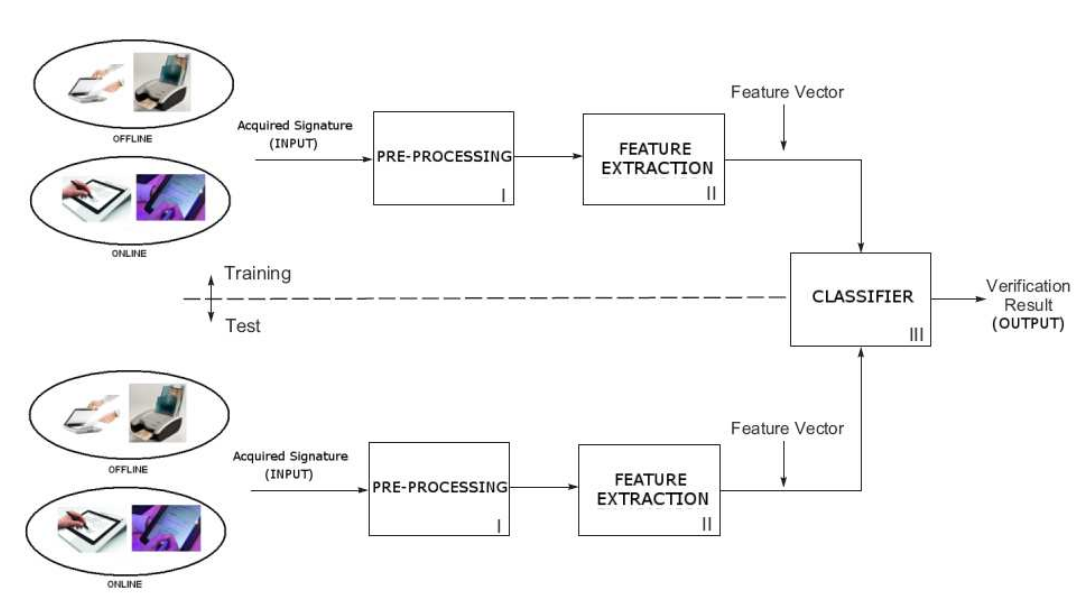
\includegraphics[width=0.65\textwidth]{imgs/vafm.png}
 \end{center}
\caption{Esquema de un sistema de VAFM. Fuente: \cite{tesis-parodi}.}
\label{fig:vafm}
\end{figure}

\begin{figure}[h!]
\begin{center}
 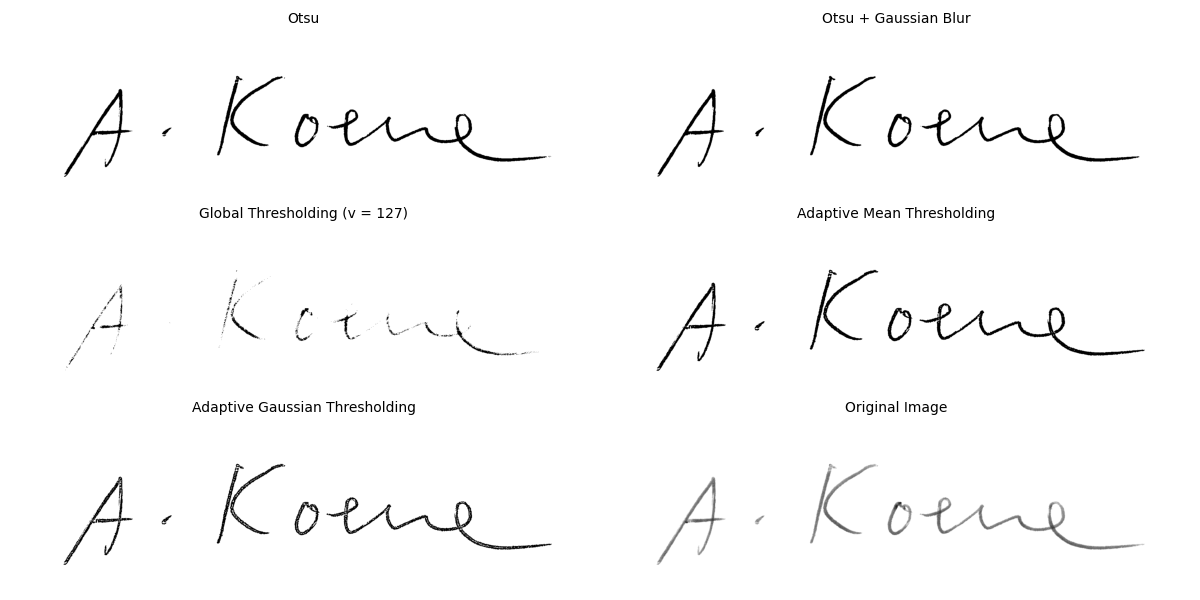
\includegraphics[width=0.9\textwidth]{imgs/image_binarization.png}
\end{center}
\caption{Distintas técnicas de preprocesamiento aplicadas a imágenes de firmas: binarización, filtros y normalización.}
\label{fig:preprocessing}
\end{figure}

Notar que se ha hecho hincapié en que este es el esquema \textit{clásico} de VAFM, entendiéndose por clásico como ``previo al Aprendizaje Profundo''. Como se explicó en la subsección \ref{subsection:representaciones}, el Aprendizaje Profundo revolucionó el paradigma del Aprendizaje Automatizado: ahora se suelen suministrar los datos crudos y es el algoritmo mismo quién aprende las características necesarias para el proceso de clasificación final.

La parte más crítica (con más impacto en los resultados) y que concentra la mayoría del conocimiento específico del dominio es la extracción de características. Es por ello que el trabajo de \cite{tesis-parodi} gira fundamentalmente en torno a esta fase.  En \cite{ip08} e \cite{ipp12} se propone gran variedad de características. La autora de \cite{tesis-parodi} ha propuesto contribuciones concernientes a la \textit{VAFM offline} en \cite{pg10a}, \cite{pg10b} y \cite{pgb11}.

\subsection{Extracción de características}

El objetivo de esta fase, que como se dijo suele ser la más importante, es encontrar una descripción adecuada de la firma.

Generalmente las características extraídas se basan en la geometría, tales como área, altura, ancho \cite{ayf90} \cite{spb94}, contorno \cite{np94}, orientación \cite{spb94}, dirección \cite{sd92}, \cite{dsg94} \cite{zna05}, la pendiente \cite{ayf90} y la curvatura \cite{jgc02} \cite{ksx04}. 

Las características descriptivas se suelen clasificar en \cite{tesis-parodi}:
\begin{itemize}
    \item \textbf{Globales:} consideran la firma como un todo. Son menos sensibles al ruido y a las variaciones de la firma \cite{hyw04}, lo cual lo hace una buen opción cuando se trabaja solamente con firmas auténticas \cite{tesis-parodi}.
    \item \textbf{Locales:} consideran partes especificas de la firma. Implica recurrir a técnicas de extracción más complejas \cite{mld11}, como por ejemplo utilizar grillas de segmentacion.
\end{itemize}

A partir de \cite{nr77} se han utilizado grillas para, a partir de ellas, extraer características locales, técnica también utilizada en \cite{sp86}, \cite{js01}, \cite{jybs00}, \cite{sjbs04}, \cite{jbs05}, \cite{ojfs05}, \cite{bzze13}.  

El trabajo de \cite{tesis-parodi} sigue esta línea proponiendo un método de grilla circular para la extracción de características locales. La idea de utilizar una grilla circular proviene de que resultan en menos sectores vacíos, además de poseer una estructura más apropiada en vistas de conseguir robustez respecto de la rotación de las firmas.

Las características propuestas en \cite{tesis-parodi} están basadas en los antecedentes de: \cite{jybs00} y \cite{js01} que utilizaron la densidad de píxeles (número de píxeles dentro de una celda), \cite{spb94} donde se calcula la distribución de píxles y \cite{jbs05} que propone utilizar el centro de gravedad (distancia del centro de gravedad en cada celda al centro de gravedad de toda la firma).

Escencialmente, \cite{tesis-parodi} ubica un esquema circular alrededor de la firma y la divide en $N$ sectores iguales, haciendo coincidir el centro de la grilla con el centro de masa de la firma (con esto se pretende la invariancia a la traslación). Luego extrae las siguientes características (ver figura \ref{fig:grillacircular}):\footnote{Notaremos $N$ el número de secciones circulares e $i$ a la $i$-ésima sección circular, con $i = 0, ..., N-1$. También referiremos con $R$ al radio de la grilla (distancia entre los dos puntos extremos).}

\begin{itemize}
    \item $x_{PD}$: Densidad de distribución de píxeles (en inglés, \textit{pixel density distributon})
    \begin{equation*}
    x_{PD_{i}} = \frac{\text{Número de píxeles negros de la sección }i}{\text{Número total de píxeles de la sección }i}
    \end{equation*}
    \item $x_{DGC}$: Distancia al centro de masa (en inglés, \textit{gravity center distance}).
    \begin{equation*}
    x_{DGC_{i}} = \frac{d_{GC_{i}}}{R}
    \end{equation*}
    Dividir por $R$ otorga cierta invarianza al escalado.
    \item $x_{AGC}$: Ángulo al centro de masa (en inglés, \textit{gravity center angle}).
    \begin{equation*}
        x_{AGC_{i}} = \frac{\alpha_{GC_{i}}}{\frac{2\pi}{N}}
    \end{equation*}
    Dividir por $\frac{2\pi}{N}$ no es estrictamente necesario, sino para lograr  escalar adecuadamente $\alpha_{GC}$ para diferentes $N$ (aunque nunca se trabajará con diferentes $N$ simultáneamente).
\end{itemize}

El vector característico es simplemente la concatenación de todas las características extraídas.

\begin{figure}[h!]
\begin{subfigure}{0.45\textwidth}
\begin{center}
 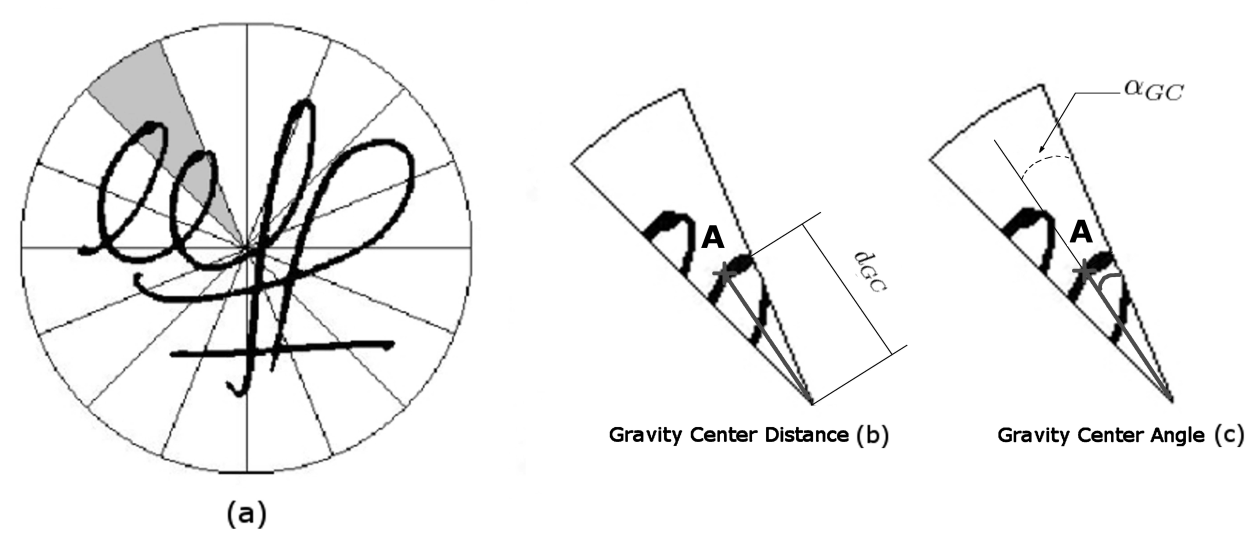
\includegraphics[width=0.85\textwidth]{imgs/grillacircular.png}
 \end{center}
\end{subfigure}
\caption{Esquema de grilla circular propuesto en  \cite{tesis-parodi}. (a) Se ha sombreado el sector analizado; (b) Distancia al centro de masa; (c) Ángulo del centro de masa. Fuente \cite{tesis-parodi}.}
\label{fig:grillacircular}
\end{figure}

\subsubsection{Invarianza rotacional mediante DFT}

Para lograr robustez frente a rotaciones, en \cite{tesis-parodi} se propone tomar los módulos de la Transformada Discreta de Fourier (DFT) de los vectores de características correspondientes a cada anillo de la grilla circular. Esta transformación produce características que son invariantes ante desplazamientos cíclicos de la secuencia original, lo cual equivale a rotaciones de la firma cuando el ángulo rotado es múltiplo de $\frac{2\pi}{N}$.

Sin embargo, cabe señalar una limitación de este enfoque: la invarianza obtenida es discreta, ya que solo se preserva ante rotaciones que correspondan exactamente al tamaño angular de una sección. Para valores pequeños de $N$ (es decir, pocas divisiones y por ende secciones angularmente grandes), las rotaciones típicas que pueden aparecer entre distintas instancias de una misma firma ---producto de variaciones en la inclinación al momento de firmar--- difícilmente coincidirán con múltiplos exactos del tamaño de sección. Esto sugiere que, en la práctica, el beneficio de esta técnica puede verse reducido cuando $N$ es pequeño.

Consideramos que el desarrollo de métodos que provean una invarianza rotacional más flexible podría resultar valioso, no solo para capturar la variabilidad intrapersonal en el ángulo de firmado, sino también porque habilitaría el uso de \textit{data augmentation} basada en rotaciones, permitiendo generar conjuntos de entrenamiento significativamente más grandes.

\subsection{Reutilizando las técnicas en nuestro problema}

\subsubsection{Entrenamiento de clasificadores y evaluación}

Recordar que en \cite{tesis-parodi} el problema a tratar consistía en verificar la identidad proclamada por el autor de cierta firma. Para ello, usa sobre dicha instancia un clasificador binario previamente entrenado para el autor que está siendo verificado, que determinará si la firma pertenece a la clase auténtica o falsa para dicha autoría. Cada clasificador (uno para cada autor) entrena la clase positiva utilizando firmas auténticas de dicho autor, y la clase negativa utilizando falsificaciones aleatorias (simuladas tomando firmas de otros autores). Esto último es muy importante debido a que, en un caso de uso real no se cuenta con falsificaciones al momento del entrenamiento. Se puede leer en detalle el protocolo de evaluación en la sección 3.5 de \cite{tesis-parodi}.

Como se dijo en la sección \ref{section:objectives}, nosotros queremos entrenar un clasificador para determinar si dos instancias de firmas son \textit{``la misma firma''} (fueron realizadas por el mismo autor). Notar que, potencialmente, los autores de las mencionadas firmas nunca han sido vistos con anterioridad por nuestro modelo. Es por ello que si bien reutilizaremos el proceso de extracción de catacterísticas con grilla circular de \cite{tesis-parodi}, no podemos entrenar un clasificador por autor.

Lo que haremos será entrenar un clasificador que reciba una combinación de las características de las imágenes de las dos firmas a analizar y determine si son o no la ``misma firma''. Para combinar los vectores característicos probaremos diferentes técnicas posibles tales como la diferencia vectorial o la concatenación de los vectores respectivos.  Nuestra metodología se explica con detalle en el capítulo siguiente, donde ahondaremos en el desarrollo de nuestros experimentos.

Nuestro problema es conceptualmente más complicado que el enfoque de \cite{tesis-parodi}, donde cada clasificador captura la varianza intrapersonal de un autor específico. La varianza intrapersonal puede diferir significativamente entre autores, por lo que construir un modelo que la capture en términos generales resulta mucho más difícil.

Más aún, la diferencia fundamental radica en que nuestra función de similaridad debe \textbf{extrapolar a autores no vistos durante el entrenamiento}. Mientras que en \textit{VAFM} se entrena un clasificador específico para cada autor (disponiendo de ejemplos de dicho autor), en nuestro caso el modelo debe aprender una noción de ``misma autoría'' lo suficientemente general como para aplicarse a firmas de personas que nunca formaron parte del conjunto de entrenamiento. Esta capacidad de generalización a nuevas identidades es lo que hace al problema intrínsecamente más difícil y lo emparenta con los problemas de \textit{One-Shot Learning} discutidos en la sección \ref{subsection:one-shot}.

\subsubsection{Métricas y convenciones}

Notar que tal como se ha explicado en la subsección \ref{subsubsection:metricasfirmas}, los conceptos $FAR$ y $FRR$ se encuentran invertidos en nuestro trabajo respecto a \cite{tesis-parodi}. Esto se debe a que nuestra clase positiva corresponde a cuando las firmas son \textit{no coincidentes} (al contrario de lo que ocurre con \cite{tesis-parodi}, donde la clase positiva concierne a que se verifica la identidad proclamada). Debemos tener en cuenta esto cuando analicemos lo resultados reportados en el mencionado trabajo para comprarlos con alguno de nuestros resultados.

Si nos fijamos en el resultado de $FAR$ de \cite{tesis-parodi}, es importante siempre considerar el respectivo a firmas ficticias, ya que como se explicó en \ref{subsection:categoria-firmas} en nuestro trabajo no utilizaremos falsificaciones simuladas.

Cabe aclarar, también, que se han utilizado conjunto de datos distintos (en el capítulo siguiente se ahondará sobre la elección y confección de los conjuntos de datos utilizados en nuestros experimentos). Y además, recalcar nuevamente que la metodología de evaluación y entrenamiento es diferente (evaluamos en firmas de autores no vistos en el entrenamiento), por lo cual el problema que nos proponemos resolver es conceptualmente mucho más difícil al de \textit{VAFM}.

\subsection{Resultados de \cite{tesis-parodi}}

Los resultados de \cite{tesis-parodi} correboran que la elección de grilla circular para el problema de \textit{VAFM} es ventajosa sobre la grilla rectangular. La grilla rectangular tiene buenos resultados de $FRR$ para número de subdivisiones grande ($N$ igual a 32, 64 o 128) pero peores resultados de $FAR$ sobre falsificaciones simples y entrenadas en dichos caso (es mejor par $N$ igual a 8). En cambio la grilla circular funciona bien en ambos casos para $N$ medianos ($N$ igual a 16), y luego empeora los resultados obtenidos al aumentar el número de subdivisiones. En \textit{tesis-parodi} se baraja la posibilidad de que esto se deba a que al aumentar las subdivisiones en la grilla circular el área de los sectores se reduce no uniformemente (al contrario de lo que sucede en la grilla rectangular). Como en nuestro trabajo no trabajaremos con falsificaciones simples (sólo con falsificaciones aleatorias como se dijo), consideraremos el grillado rectangular con $N$ grande ($N$ igual a 128), ya que en dicho casos muestra buenos resultados de $FAR$ en \cite{tesis-parodi}.

Finalmente los mejores resultados reportados en \cite{tesis-parodi} corresponden a las siguientes configuraciones:

\begin{table}[h!]
\begin{tabular}{l|c|c|l}
\cline{2-3}
\textbf{}                                              & \begin{tabular}[c]{@{}c@{}}Grilla circular\\ N=16, Kernal polinómico\end{tabular} & \begin{tabular}[c]{@{}c@{}}Grilla rectangular\\ N=128, Kernel RBF\end{tabular} &  \\ \cline{1-3}
\multicolumn{1}{|l|}{FRR}                              & 18.75 \%                                                                          & 27.875 \%                                                                      &  \\ \cline{1-3}
\multicolumn{1}{|l|}{FAR (firmas ficticias)}           & 0.0727 \%                                                                         & 0.0106 \%                                                                      &  \\ \cline{1-3}
\multicolumn{1}{|l|}{FAR (fals. simples y entrenadas)} & 2.125 \%                                                                          & 14.9167 \%                                                                     &  \\ \cline{1-3}
\end{tabular}
\end{table}

Nuestros objetivos, mencionados en \ref{subsubsection:costo-beneficio},



Notar que ninguno de los resultados exhibidos satisface (si bien está cerca) nuestra meta de lograr un \textit{recall} de al menos 0.8 y \textit{precision} de 0.95 mencionada en . De todos modo, cabe recordar las limitaciones expuestas en secciones anteriores sobre extrapolar los citados resultados a nuestro trabajo.

\subsubsection{Críticas metodológicas}

En los siguientes apartados expresamos algunas críticas al trabajo analizado. Entenderlas y analizarlas nos es útil para interpretar los resultados correctamente. Y también nos ha ayudado en el diseño correcto de nuestro protocolo de evaluación (capítulo siguiente).

\paragraph{Desbalance en el conjunto de datos de entrenamiento}\mbox{}\\

La clase verdadera de cada autor es entrenada con 14 firmas auténticas, mientras que la clase falsa es entrenada con firmas auténticas de otros autores.

El desbalance de clases es muy significativo y esto puede generar (depende de la configuración de entrenamiento de las SVM) un sesgo a favor de reducir el FAR sobre el FRR. Lamentablemente no tenemos acceso al código de los experimentos para constatar si se ha tomado alguna medida para mitigar el desbalance, como ponderar las clases a la hora de entrenar las SVM.

Este problem fue anoticiado por la autora en las conclusiones de la sección 3.9 \cite{tesis-parodi}.

\paragraph{Error metodológico en la evaluación de firmas ficticias}\mbox{}\\

El trabajo reporta resultados de $FAR$ para firmas ficticias. Para calcularlo utiliza firmas auténticas de los otros autores. Estas firmas provienen del conjunto de evaluación, o sea que no han sido utilizadas durante el entrenamiento.

Pese a que a primeras vistas puede parecer correcto tiene un sutil pero severo error: los autores de estas firmas sí han sido potencialmente usados para entrenar la clase falsa del clasificador que está siendo evaluado. Por lo qué el clasificador conoce firmas parecidas para la clase falsa. 

Naturalmente, esta correlación oculta podría no repetirse en un caso real. Ya que las falsificaciones simuladas no necesariamente se parecerán a ninguna de las firmas falsas que ha visto el clasificador durante el entrenamiento.

No podemos decir con certeza que no se hayan tomado recaudos frente a esta situación, como evaluar el $FAR$ de firmas ficticias para cada clasificador en autores que no se hayan utilizado para entrenar, porque no tenemos acceso al código de los experimentos. No obstante, como el protocolo de evaluación (sección 3.5 de \cite{tesis-parodi}) no hace salvedad alguna, pensamos que es probable que no se haya anoticiado de este error.

Es por este error que podemos sospechar que el $FAR$ de firmas ficticias es demasiado optimista.

\paragraph{Desbalance en el conjunto de datos de evaluación}\mbox{}\\

En la sección 3.5 de \cite{tesis-parodi} (\textit{``Protocolo de evaluación''}), se explica que para la fase de test se utilizan

\section{Conjuntos de datos}

\subsection{GPDS300}

Observaciones a su proceso de evaluación y conclusiones
En [TESIS-MARIANELA] se utilizó la base de datos GPDS300 Signature CORPUS [VFTA07]. Por regulaciones de la UE ya no se encuentra disponible para su uso. La base contaba con 160 escritore, 24 firmas auténticas y 30 falsificaciones por autor.


Fue el utilizado en \cite{tesis-parodi}. %Es presentado en \cite{vfta07}.

En [TESIS-MARIANELA] se utilizó la base de datos GPDS300 Signature CORPUS [VFTA07]. Por regulaciones de la UE ya no se encuentra disponible para su uso. En la página de GPDS (grupo de procesamiento de señales) existe actualmente un dataset sintético.
En la Conferencia Internacional sobre Análisis y Reconocimiento de Documentos (ICDAR por sus siglas en ingles) se han realizado competencias de vital importancia al área brindando a los investigadores la posibilidad de comparar el rendimiento de sus sistemas y proponer desafíos interesantes en sus datasets. 



La organización de estas competencias es de vital importancia para el área ya que
no sólo brinda a los investigadores la posibilidad de comparar el rendimiento de
sus sistemas, sino también de testear sus algoritmos con bases de datos estándar
y al alcance de toda la comunidad.
Además, las bases de datos presentadas en
el marco de las competencias suelen proponer desafíos interesantes. Por ejemplo,
para las competencias llevadas a cabo durante ICDAR 2009 y ICDAR 2011, se
construyó una base de datos conteniendo firmas de origen chino, mientras que
para la competencia llevada a cabo durante ICDAR 2013 se introdujo una base
de datos conteniendo firmas de origen japonés. Además de las competencias, en
los últimos años se organizaron distintos talleres y tutoriales en el marco de las
mencionadas conferencias. Estas reuniones periódicas permiten discutir los as-
pectos emergentes del área, brindándoles a los investigadores la oportunidad de
intercambiar ideas y discutir su trabajo actual en un contexto informal y disten-
didp.

Los primeros dos son de las competencias organizadas por ICDAR (International Conference on Document Analysis and Recognition).
La ventaja es que se consigue fácil tanto el dataset como el papper con los resultados. Ademas hay dando vueltas implementaciones (que no probé) de gente que se tiró a resolver esos dataset.
SigComp2011 tiene firmas occidentales (alemanas) y orientales (chinas) yo usaria solo las occidentales.
SigComp2009 tiene ~1800 firmas (entre autenticas y falsificaciones)
SigComp2011 tiene ~400 firmas occidentales (entre autenticas y falsificaciones).
Yo me tiraría a usar la 2009 porque tiene más. Aunque la otra es un poco más nueva.

La que usa Marianela en su tesis es GPDS960 pero no está disponible por una resolución de privacidad de la UE (ver la fuente). En internet tampoco la encontré (no busqué mucho tampoco).
La pagina sugiere usar las bases de datos sintéticas que listé abajo. A mí no me gustó el hecho de que sea sintética, aunque deben estar bien generadas, hay un paper y todo. Otro contra es que hay que llenar un formulario y mandarlo, no es tan simple como poner descargar. Lo bueno de esa opción es que son muchísimas como 4000.
Tampoco pude encontrar gratis el papper de este último dataset "Off-line handwritten SignatureGPDS-960 Corpus." F. Vargas, M.A. Ferrer, C.M. Travieso, and J.B. Alonso.


Los conjuntos de datos utilizados Sigcomp 2009 \cite{sigcomp2009} y Sigcomp 2011 \cite{sigcomp2009}, provienen de las competencias llevadas a cabo durante las ediciones 2009 y 2011 respectivamente de la International Conference on
Document Analysis and Recognition (ICDAR).

Las competencias presentan base de datos interesantes y permiten a los investigadores del área la posibilidad de comparar su rendimiento de manera estándar \cite{tesis-parodi}.



\section{Problemas de similitud}

\subsection{Problemas clásicos similares: \textit{Face Recognition} y \textit{Face Verification}}

Los rostros, al igual que las firmas, son una característica biométrica que puede ser utilizada para la autenticación. No es de sorprender, entonces, que los mismos problemas que atañen a firmas tengan su paralelismo con el procesamiento de imágenes de rostros. En ambos casos resulta fundamental extraer características discriminativas que permitan clasificar o comparar instancias provenientes de distintas personas.

El problema de \textbf{\textit{Face Verification}} consiste en verificar si un cierto rostro pertenece a una determinada persona (de la cual se conocen rostros). La entrada es una imagen del rostro junto con la identidad declarada, y la salida del modelo es un booleano indicando si la imagen corresponde efectivamente a dicha persona:

\begin{equation*}
    Face \ Verification \ System (face\_image, \ person\_id ) : Bool
\end{equation*}

En contraste, en el problema de \textit{\textbf{Face Recognition}} sólo se posee una imagen y se debe detectar si el rostro corresponde a alguna persona de una base de datos de rostros conocidos. Es decir, la entrada es únicamente la imagen del rostro y la salida es la identidad correspondiente (o ``no reconocido'' si no coincide con ninguno de la base de datos):

\begin{equation*}
    Face \ Recognition \ System (face\_image) :  Person \ ID \cup \{ Not\ Recognized \}
\end{equation*}

Notar que si bien el problema de \textit{Face Recognition} parece más difícil que el de \textit{Face Verification}, una solución a este último con suficiente precisión, se puede trasladar al segundo iterando para identidad posible de la base de datos.

\subsection{\textit{One-Shot Learning}} \label{subsection:one-shot}

La mayor dificultad de ambos problemas es que generalmente consisten en problemas de \textbf{\textit{One-Shot learning}} (o \textit{Few-Shot learning}):
\begin{itemize}
    \item El conjunto de entrenamiento cuenta con un (o unos pocos) ejemplos para cada categoría (persona o identidad en el caso de rostros).
    \item Existen a su vez muchas etiquetas (muchas personas distintas). Y además pueden agregarse nuevas e idealmente no queremos re-entrenar todo el modelo cada vez que esto ocurra.
\end{itemize}
De estas restricciones se desprende que no será útil atacar el problema utilizando un clasificador donde haya una clase por identidad, ya que al poseer pocos ejemplos de cada clase, el entrenamiento lograría una muy pobre precisión. Además, este enfoque obligaría a re-entrenar el modelo cada vez que se quiera agregar una nueva persona. \\
En vez de esto, una solución posible es aprender una función de similaridad $d$:
\begin{equation*}
    d(img_1, img_2) = \text{grado de diferencia entre ambas personas}
\end{equation*}
Luego, podemos resolver \textit{Face Verification} comparando la salida de $d$ respecto de un umbral $\tau$: 

\begin{equation*}
    d(img_1, img_2) \left\{ \begin{array}{lcc}
             \leq \tau &   si  & id(img_1) = id(img_2) \\
             \\ > \tau &   si  & id(img_1) \neq id(img_2) 
             \end{array}
   \right.
\end{equation*}

De este modo resolvemos un problema ``más fácil'' que el de reconocer la identidad de cada sujeto (el modelo tiene disponible en su valuación la imágen contra la cuál está comparando). 

Además, con este enfoque de aprender una función de similaridad de rostros $d$ generalizable a identidades no vistas sobre el entrenamiento, no necesitaremos re-entrenar el modelo de agregarse nuevas personas a la base de datos.

\subsection{\textit{Redes Siamesas}}

La arquitectura que se emplea para esta clase de problemas es conocida como \textbf{\textit{Redes Siamesas}} \cite{siamess-lecun}. Consiste en utilizar una red convolucional clásica (una sucesión de convoluciones y capas de \textit{pooling}) y valerse de las activaciones de entrada de la última capa (la predicción) como vector de características (también llamado \textbf{\textit{embedding}} o \textbf{\textit{encoding}} de la imagen). Para finalmente calcular la similitud como la distancia entre ambos \textit{embeddings}. Ver figura \ref{img:siamess}. En la figura \ref{fig:signatures_paired} se muestra un ejemplo de cómo se estructura un dataset pareado para entrenar estas redes.

\begin{figure}[h]
\centering
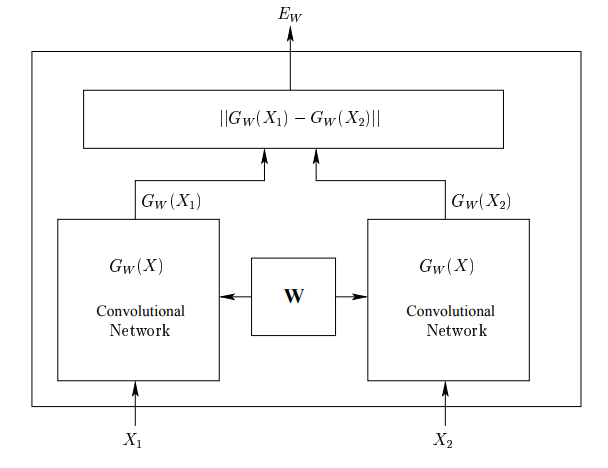
\includegraphics[width=0.7\textwidth]{imgs/siamess.png}
\caption{Arquitectura general de una \textit{Red Siamesa}. Fuente: \cite{siamess-lecun}}
\label{img:siamess}
\end{figure}

\begin{figure}[h]
\centering
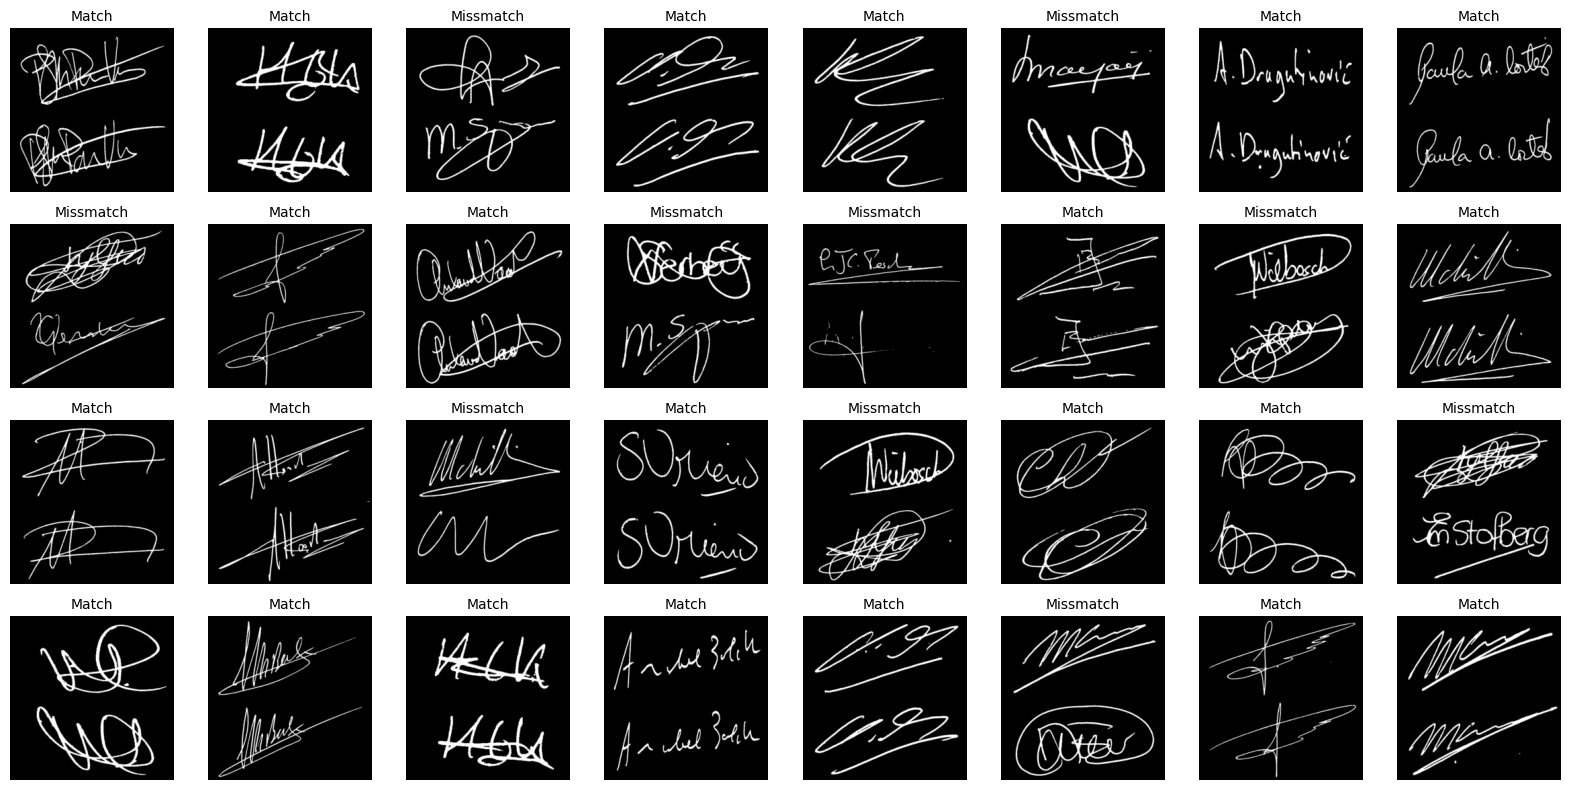
\includegraphics[width=0.9\textwidth]{imgs/signatures_paired.png}
\caption{Ejemplo de un dataset pareado de firmas: cada instancia consiste en un par de firmas junto con un veredicto indicando si corresponden o no al mismo autor.}
\label{fig:signatures_paired}
\end{figure}

Notar que en el cálculo de los \textit{embeddings} de ambas imágenes se utilizan los mismos pesos (notado como $W$ en la figura \ref{img:siamess}). Esta técnica dónde los mismos parámetros se reutilizan, en dos o más cómputos diferentes, en cada evaluación del modelo, se suele denominar \textit{Tied Weights} en la jerga del \textit{aprendizaje profundo}.


En línea con la figura \ref{img:siamess}, notaremos con $G_W$ la función definida al aplicar nuestro modelo (también llamado \textit{encoder}). Siendo  entonces $G_W(img)$ el \textit{encoding} o \textit{embedding} de la imagen $img$ utilizada.

Para comparar los \textit{embeddings} pueden utilizarse diferentes funciones distancia (la distancia coseno, la euclídea y $\mathcal{X}^2$ están entre las más escogidas). 

El entrenamiento debiera optimizar el \textit{encoder} $G_W$, hallando valores de $W$ óptimos, para extraer características útiles a la hora de comparar dos imágenes (rostros en el caso del problema de \textit{Face Verification}). Notar que este es un claro ejemplo de lo discutido en \ref{subsection:representaciones} donde se utiliza redes neuronales para aprender las características útiles a extraer, en vez de codificarlas a mano (las cuáles probablemente son dependiente del dominio de las imágenes a comparar).
Más formalmente, el entrenamiento deberá aprender parámetros del \textit{encoder} tal que:
\begin{equation*}
    ||~G_W(img_1) - G_W(img_2)~||_2 < \tau \Longleftrightarrow{} \text{id}(img_1) = \text{id}(img_2) 
\end{equation*}

Notar la importancia para el desarrollo del \textit{Aprendizaje Profundo} de la funcionalidad de diferenciación automática (también llamada \textbf{\textit{Autograd}}) de los \textit{frameworks} como \textit{Pytorch} o \textit{TensorFlow}: cuestiones como \textit{Tied Weights} en la formulación del costo hacen que las expresiones de los gradientes sean complicadas de tener que calculárselas manualmente. Afortunadamente, las librerías encapsulan dicho problema y los mismos son computados automáticamente. Lo que da pie a que se experimente con formulaciones más complejas y da lugar a entrenamientos más sofisticados.

\subsection{}

Resta definir la función de costo

\subsection{\textit{Image Similarity}}

\subsection{\textit{Omniglot Dataset}}

\chapter{Experimentos} \label{chapter:experimentos}

\section{Formulación del problema en la práctica}

En este capítulo describimos cómo se lleva a la práctica la formulación presentada en el capítulo \ref{formulacion-del-problema}: el problema a resolver es determinar si dos firmas son de la misma autoría, con el fin de detectar errores de confección en los telegramas electorales que tienen varias páginas y donde las firmas deben coincidir entre página y página. Un ejemplo de telegrama real puede verse en \url{https://drive.google.com/file/d/1X36KFIH7QEQzfrL6or0WEYuK1FaxuMsS}. 

De acuerdo con los objetivos definidos en la sección \ref{section:objectives}, buscamos maximizar la \textit{precision} sujeta a obtener un \textit{recall} no menor que $0.9$. Para ello nos basamos en trabajos anteriores de problemas similares y, en particular, utilizamos la tesis de Parodi \cite{tesis-parodi} como principal punto de comparación. La tesis de Parodi resuelve el problema de \textit{VAFM} (\textit{Verificación Automática de Firmas Manuscritas}), donde se dispone de $K$ autores y, dada una firma que declara ser de un autor $i$, se debe verificar su autenticidad entrenando un clasificador por autor. En nuestro caso el enfoque es distinto: queremos detectar errores de confección y no falsificaciones, por lo que no consideramos firmas falsificadas (hechas por un autor pretendiendo ser otro), sino únicamente firmas auténticas y sus combinaciones. 

El problema es conceptualmente cercano al reconocimiento facial (\textit{Face Recognition}/\textit{Face Verification}), donde también se comparan instancias biométricas de distintas personas. En los experimentos aprovechamos ideas de la literatura de reconocimiento facial y de redes siamesas desarrolladas por grandes actores de la industria (por ejemplo, trabajos recientes sobre reconocimiento de caras basados en redes convolucionales profundas).

\section{Conjuntos de datos}

\subsection{Conjuntos de datos curados}

En una primera etapa no contamos con un \textit{dataset} de pares de firmas listo para usar, sino con una colección de telegramas. Para acotar el problema de similaridad de firmas y poder comparar los resultados con soluciones existentes, trabajamos inicialmente con \textit{datasets} curados de firmas manuscritas y recién luego nos movemos al conjunto de datos generado por nosotros.

Uno de los conjuntos de datos considerados es \textbf{CEDAR Signature}\footnote{Disponible, por ejemplo, en repositorios como \url{https://paperswithcode.com/dataset/cedar-signature}.}, que contiene 1\,320 firmas de 55 autores (24 auténticas por autor) y 1\,320 falsificaciones. Siguiendo los criterios de nuestro problema, no utilizamos las falsificaciones directamente, sino que generamos pares negativos (\textit{falsos matcheos}) combinando firmas auténticas de distintos autores.

Otro conjunto de datos utilizado es \textbf{SigComp 2009}, que fue desarrollado para la competencia de verificación de firmas del ICDAR 2009. Este conjunto se divide en dos partes: un subconjunto de entrenamiento y uno de evaluación, provistos por instituciones distintas.

\paragraph{SigComp 2009 Train (NISDICC).} El subconjunto de entrenamiento fue proporcionado por el \textit{National Institute of Standards and Technology} (NIST) y el \textit{Document Image and Character Collection} (DICC). Contiene firmas de 12 autores auténticos (identificados como 001--012) y 31 falsificadores (021--051). Cada autor auténtico firmó 5 originales, y en general cada falsificador realizó 5 falsificaciones por autor auténtico; sin embargo, hay falsificaciones faltantes (1\,898 archivos en lugar de 1\,920). Las imágenes tienen diferentes tamaños y están en escala de grises.

\paragraph{SigComp 2009 Test (NFI).} El subconjunto de evaluación fue proporcionado por el \textit{Netherlands Forensic Institute} (NFI). Contiene firmas de autores identificados del 001 al 100, aunque muchos identificadores no están presentes. No todos los autores son falsificadores (la cantidad de falsificadores es menor que la cantidad de autores). En general, cada autor auténtico firmó 12 originales (algunos firmaron 11 y uno firmó 6), y cada falsificador realizó 6 falsificaciones para 2--4 autores auténticos. También hay falsificaciones faltantes (1\,564 archivos en lugar de 1\,953). Las imágenes tienen diferentes tamaños y están en escala de grises.

\subsection{Confección del \textit{dataset} propio (cropeo de firmas)}

\textcolor{red}{\textbf{TODO:} Mencionar que detectar firmas en ubicaciones arbitrarias o segmentar qué píxeles pertenecen a cada firma es un problema en sí mismo, que no abordamos aquí gracias a que la estructura del telegrama es fija. Citar \cite{handwritten-text-segmentation} como referencia al problema de segmentación de texto manuscrito.}

Para evaluar los modelos en un escenario más cercano a la aplicación real, construimos un conjunto de datos propio a partir de telegramas electorales. Inicialmente no contamos con un \textit{dataset} propiamente dicho (de pares de firmas, ni siquiera de firmas aisladas), sino con imágenes completas de telegramas. Aprovechamos que la localización de las firmas en el formulario es fija para extraerlas mediante recortes sobre el telegrama. Luego, para detectar si hay o no hay firma en dicha posición, probamos primero una heurística sencilla basada en el tamaño de las componentes conexas (alrededor de 0.90 de \textit{accuracy}); tras una revisión manual rápida de la clasificación obtenida y algunas correcciones, entrenamos un clasificador de redes neuronales que alcanzó aproximadamente 0.99 de \textit{accuracy}. Esto ilustra cómo un modelo puede servir como herramienta para un paso intermedio de limpieza y construcción del \textit{dataset}.

\section{Resultados}

En todas las gráficas de métricas (por ejemplo, curvas ROC y Precision--Recall) fijamos la escala de los ejes $x$ e $y$ en el intervalo $[0, 1]$ para que las comparaciones entre modelos sean coherentes y visualmente consistentes. Además, para comparar de forma resumida el desempeño entre distintas particiones de validación cruzada reportamos también la métrica $F_1$, definida como la media armónica entre \textit{precision} y \textit{recall}.

\subsection{Resultados utilizando la tesis de Marianela}

En primer lugar reproducimos, en la medida de lo posible, el esquema basado en extracción de \textit{features} manuales propuesto en \cite{tesis-parodi}, utilizando los descriptores construidos sobre grillas y entrenando clasificadores como \textit{Random Forest} o SVM sobre los vectores característicos. Sobre el conjunto de datos de referencia SigComp2009 se obtiene, por ejemplo, una \textit{performance} del orden de $0.85$ para la métrica de interés combinando extracción de características manual (Parodi) con \textit{Random Forest}.

\subsection{Resultados utilizando redes siamesas}

Como siguiente paso entrenamos redes siamesas convolucionales que reciben pares de recortes de firmas y producen un puntaje de similitud a partir de la distancia entre sus \textit{embeddings}, tal como se describe en la subsección \ref{subsection:siamesas}. Aquí se incluirán los resultados cuantitativos comparables con el enfoque basado en \cite{tesis-parodi} (falta completar esta parte con los valores finales de \textit{precision}, \textit{recall} y curvas ROC / Precision--Recall).

\subsection{Resultados con diferentes arquitecturas de redes siamesas}

Exploramos diferentes arquitecturas convolucionales para el \textit{encoder} $G_W$ (variando profundidad, número de filtros y uso de bloques residuales tipo ResNet) y analizamos su impacto sobre las métricas de similitud. Esta sección detalla comparaciones entre arquitecturas más pequeñas y más profundas, así como el efecto de utilizar modelos preentrenados y \textit{fine-tuning} (resta completar con los experimentos definitivos).

\subsection{Online triplet loss y offline triplet loss}

Finalmente entrenamos modelos siameses utilizando \textit{triplet loss} (ver \ref{subsubsection:triplet-loss}), comparando estrategias de generación de tripletas \textit{offline} (precomputadas) y \textit{online} (minado de tripletas dentro de cada \textit{mini-batch}). El conjunto de datos se genera particionando autores entre entrenamiento y test (no se mezclan firmas de un mismo autor entre ambos, y se utilizan únicamente firmas originales, no falsificaciones). En esta sección se reportan las métricas alcanzadas por cada estrategia y se discuten sus ventajas prácticas en términos de estabilidad de entrenamiento y capacidad de generalización (pendiente de completar con los números finales).



% Apéndices
\chapter{Conclusiones}

En esta tesina se planteó el problema de detectar automáticamente inconsistencias en las firmas manuscritas de los telegramas electorales utilizados en el escrutinio provisorio con asistencia digital en la Provincia de Santa Fe. A diferencia del enfoque clásico de VAFM, el objetivo no fue identificar falsificaciones intencionales, sino errores de confección (ausencia de firmas o firmas no coincidentes entre páginas) que derivan en retransmisiones y trabajo adicional en el centro de cómputo. El problema se formalizó como una tarea de clasificación binaria sobre pares de imágenes de firmas, definiendo cuidadosamente las métricas de evaluación (\textit{precision}, \textit{recall}, curvas ROC / Precision–Recall) y el rol asimétrico de los errores según el uso práctico del sistema. 

Desde el punto de vista metodológico, se construyó primero un conjunto de datos propio a partir de telegramas reales, aprovechando que el diseño de los formularios es conocido de antemano. Se diseñó un pipeline donde, a partir de fotografías de telegramas, se recortan automáticamente las zonas de firmas y se entrena un modelo intermedio para detectar presencia/ausencia de firma, que permitió limpiar y estructurar el conjunto de datos definitivo. Sobre este \textit{dataset} se compararon dos familias de enfoques: (i) métodos “clásicos” basados en extracción manual de características (grillas y descriptores inspirados en \cite{tesis-parodi}) combinados con clasificadores como Random Forest y SVM; y (ii) modelos de Aprendizaje Profundo basados en redes convolucionales y arquitecturas siamesas para aprendizaje de representaciones y métricas de similitud. 

Los experimentos muestran que las redes siamesas convolucionales, entrenadas con funciones de costo específicas para aprendizaje de métricas (como \textit{triplet loss} en variantes \textit{online} y \textit{offline}), logran resultados claramente superiores a los enfoques basados en características manuales, tanto en conjuntos de datos estándar de firmas como en el escenario particular de los telegramas. Se alcanzan configuraciones de operación donde el modelo mantiene un \textit{recall} en torno a 0.8–0.9 con alta \textit{precision}, lo que en términos prácticos se traduce en una reducción significativa del número de retransmisiones por errores de firmas, manteniendo a la vez un volumen limitado de falsas alarmas aceptable para el flujo de trabajo del centro de cómputo. 

Como principales limitaciones se destaca la dependencia del modelo respecto del formato de los telegramas (posición fija de las firmas y calidad de las imágenes), la ausencia de falsificaciones intencionales en el conjunto de datos (el foco está puesto en errores de confección) y la necesidad de contar con volúmenes suficientes de datos etiquetados para explorar arquitecturas más grandes. En el capítulo de Trabajo futuro se discuten posibles extensiones, entre ellas: el uso de representaciones aprendidas mediante modelos generativos (autoencoders o GANs), la exploración de arquitecturas siamesas y de \textit{metric learning} más modernas, y la adaptación del pipeline a otros problemas de similitud de imágenes, como verificación de identidad en documentos o análisis de otras marcas manuscritas. Estas líneas abren el camino para seguir mejorando la robustez y capacidad de generalización del sistema propuesto.



\appendix

\chapter{Construcción del conjunto de datos}

Resultados al problema de presencia de firmas


Resultados al problema de similaridad entre firmas
- Conjunto de datos
	- Sigcomp 2009 (citar y explicar brevemente)
	- CEDAR (citar y explicar brevemente)
	- Conjunto de datos propios a partir de telegramas
	(como lo construí)
		- recortar
		- filtrar los lugares donde no aparecen firmas usando la solucion anterior
		- matchear los cuadraditos entre diferentes paginas
- Soluciones planteadas
	- Approach I (nuestra implementacion a lo de marianela)
	- Approach II (deep learning)
- Experimentos y resultados
	- Experimentos planteados (1,2,3,4)
	- Resultados respectivos


Se obtiene el conjunto de datos crudo sobre el cual se desea aprender. Los datos son la base del proceso y condicionarán todo el trabajo posterior. No es trivial controlar de qué manera son recolectados.
En la academia se suelen utilizar conjuntos de estándares para los cuales por lo general existen publicaciones que detallan sus características. De este modo se garantiza que se trabaja con datos que han sido rigurosamente extraídos (por ejemplo si se trata de texto manuscrito se detalla el espesor del bolígrafo, el tipo de superficie sobre la cual se escribe, la posición respecto a los renglones, la distribución en género/edad de los voluntarios a escribir, etc). Generalmente se trata de que posean características tales que los resultados de las investigación sobre ellos puedan extrapolarse a conjuntos de datos del mismo tipo.
Además se cuenta con de conjuntos de datos estándares que permite a los científicos comparar sus resultados.
En trabajos de aplicación (como en la industria), es un paso muy importante que muchas veces se descuida. Una extracción incorrecta de los datos podría introducir errores en el entrenamiento difíciles de detectar. Es importante que se realice de forma iterativa y siempre visualizando los conjuntos de datos generados para garantizar una relativa sanidad de los mismos.
Un ejemplo frecuente cuando se enseña \textit{Machine Learning} es el del entrenamiento de un detector de tanques de guerra camuflados que a primeras vistas poseía una asombrosa precisión pero luego resultó estar detectando presencia de nubes en el cielo: las fotos del escenario con los tanques habían sido tomadas un día soleado y las fotos sin los tanques un día nublado. Aparentemente esta situación anecdótica constituye un mito urbano del \textit{Machine Learning}, ver [CITA GWERN https://www.gwern.net/Tanks\#should-we-tell-stories-we-know-arent-true]. Aunque en la misma fuente se pueden encontrar ejemplos documentados de errores de generalización en aplicaciones de \textit{Machine Learning} producto de haber entrenado con \textit{datasets} sesgados.

En nuestra implementación que sigue un enfoque clásico basándonos en \cite{tesis-parodi} utilizaremos para la fase de clasificación \textit{SVM} para la extracción de características el método de grilla circular que explicaremos en las subsecciones siguientes \textit{SVM} cuando tratemos con el enfoque clásico y usemos 

Del mismo modo es muy importante definir bien el formato de los datos (ver si se trata de un problema de regresión una clasificación y en último caso definir bien las clases)


\chapter{Trabajo futuro}
detectar suplantaciones



\clearpage

\textcolor{red}{Ordenar alfabeticamente la bibliografia}




\begin{thebibliography}{9}

\bibitem[Hao Li et al. 2018]{visualizing-landscapes}
Hao Li, Zheng Xu, Gavin Taylor, Christoph Studer, Tom Goldstein. (2018).
\textit{Visualizing the Loss Landscape of Neural Nets}.
University of Maryland, College Park United States Naval Academy Cornell University.

\bibitem[Dauphin et al. 2014]{no-chair}
Yann N. Dauphin et al. (2014).
\textit{Identifying and attacking the saddle point problem in high-dimensional non-convex optimization}.
Advances in Neural Information Processing Systems, pp. 2933-2941.

\bibitem[Nielsen 2015]{libro-nielsen}
Nielsen, M. A. (2015).
\textit{Neural Networks and Deep Learning}.
Determination Press.

\bibitem[Ruder 2016]{compare-optimizers}
Sebastian Ruder. (2016).
\textit{An overview of gradient descent optimization algorithms}.
arXiv: 1609.04747 [cs.LG].

\bibitem[Xu et al. 2015]{leaky-relu2}
Xu, B., Wang, N., Chen, T., and Li, M. (2015).
\textit{Empirical evaluation of rectified activations in convolutional network}.
CoRR, abs/1505.00853.

\bibitem[Maas et al. 2013]{leaky-relu1}
Maas, A. L., Hannun, A. Y., and Ng, A. Y. (2013).
\textit{Rectifier nonlinearities improve neural network acoustic models}.
In ICML Workshop on Deep Learning for Audio, Speech and Language Processing.

\bibitem[Nair and Hinton 2010]{relu-def}
Nair, V. and Hinton, G. E. (2010).
\textit{Rectified linear units improve restricted boltzmann machines}.
In Proceedings of the 27th International Conference on Machine Learning (ICML-10), pp. 807–814.

\bibitem[Deng et al. 2009]{imagenet}
Deng, J., Dong, W., Socher, R., Li, L.-J., Li, K., and Fei-Fei, L. (2009).
\textit{ImageNet: A large-scale hierarchical image database}.
2009 IEEE Conference on Computer Vision and Pattern Recognition.

\bibitem[Glorot et al. 2011]{relu-biology}
Glorot, X., Bordes, A., and Bengio, Y. (2011).
\textit{Deep sparse rectifier neural networks}.
In Proceedings of the 14th International Conference on Artificial Intelligence and Statistics, pp. 315-323.

\bibitem[Krizhevsky et al. 2012]{relu-fast}
Krizhevsky, A., Sutskever, I., and Hinton, G. E. (2012).
\textit{Imagenet classification with deep convolutional neural networks}.
In Advances in Neural Information Processing Systems, pp. 1097-1105.

\bibitem[Wolpert 1996]{limitation-aprox}
Wolpert, D. H. (1996).
\textit{The lack of a priori distinctions between learning algorithms}.
Neural Computation, 8(7), pp. 1341-1390.

\bibitem[Goodfellow et al. 2016]{deeper-better}
Goodfellow, I., Bengio, Y., and Courville, A. (2016).
\textit{Deep Learning}.
MIT Press.

\bibitem[LeCun et al. 2015]{lecun-dl}
LeCun, Y., Bengio, Y., and Hinton, G. (2015).
\textit{Deep learning}.
Nature, 521(7553), p. 436.

\bibitem[Rumelhart et al. 1986]{momentum}
Rumelhart, D. E., Hinton, G. E., and Williams, R. J. (1986).
\textit{Learning representations by backpropagating errors}.
Nature, 323(9).

\bibitem[Hinton 2014]{rmsprop}
Hinton, G. (2014).
\textit{Neural Networks for Machine Learning}.
Coursera course.
\url{http://www.cs.toronto.edu/~tijmen/csc321/slides/lecture_slides_lec6.pdf}

\bibitem[Kingma and Ba 2014]{adam}
Kingma, D. P. and Ba, J. (2014).
\textit{Adam: A method for stochastic optimization}.
CoRR, abs/1412.6980.

\bibitem[He et al. 2015]{kaiming-init}
He, K., Zhang, X., Ren, S., and Sun, J. (2015).
\textit{Delving Deep into Rectifiers: Surpassing Human-Level Performance on ImageNet Classification}.
\url{https://arxiv.org/abs/1502.01852}

\bibitem[Glorot and Bengio 2010]{xavier-init}
Glorot, X. and Bengio, Y. (2010).
\textit{Understanding the difficulty of training deep feedforward neural networks}.
DIRO, Université de Montréal, Montréal, Québec, Canada.
\url{http://proceedings.mlr.press/v9/glorot10a/glorot10a.pdf}

\bibitem[Ioffe and Szegedy 2015]{batch-normalization}
Ioffe, S. and Szegedy, C. (2015).
\textit{Batch Normalization: Accelerating Deep Network Training by Reducing Internal Covariate Shift}.
\url{https://arxiv.org/abs/1502.03167}

\bibitem[Srivastava et al. 2014]{dropout}
Srivastava, N., Hinton, G., Krizhevsky, A., Sutskever, I., and Salakhutdinov, R. (2014).
\textit{Dropout: A Simple Way to Prevent Neural Networks from Overfitting}.
Journal of Machine Learning Research, 15, pp. 1929-1958.
\url{https://arxiv.org/pdf/1207.0580.pdf}
 
\bibitem[Loshchilov and Hutter 2019]{decouple-weight-decay}
Loshchilov, I. and Hutter, F. (2019).
\textit{Decoupled Weight Decay Regularization}.
In International Conference on Learning Representations (ICLR).
\url{https://arxiv.org/pdf/1711.05101.pdf}

\bibitem[Krogh and Hertz 1991]{weight-decay} 
Krogh, A. and Hertz, J. (1991).
\textit{A Simple Weight Decay Can Improve Generalization}.
Advances in Neural Information Processing Systems 4 (NIPS 1991).

\bibitem[LeCun 1989]{lecun-invariance-shift} 
LeCun, Y. (1989).
\textit{Generalization and Network Design Strategies}.
Department of Computer Science, University of Toronto.

\bibitem[LeCun et al. 1998]{lenet} 
LeCun, Y., Bottou, L., Bengio, Y., and Haffner, P. (1998).
\textit{Gradient-Based Learning Applied to Document Recognition}.
Proceedings of the IEEE, 86(11), pp. 2278-2324.

\bibitem[Cybenko 1989]{universal-width} 
Cybenko, G. (1989).
\textit{Approximation by superpositions of a sigmoidal function}.
Mathematics of Control, Signals, and Systems, 2(4), pp. 303–314.

\bibitem[Rumelhart et al. 1986a]{backpropagation3} 
Rumelhart, D. E., Hinton, G. E., and Williams, R. J. (1986a).
\textit{Back-Propagation and Other Differentiation Algorithms}.
In Parallel Distributed Processing, Vol. 1, Chapter 6.5, pp. 200–220.

\bibitem[Rumelhart et al. 1986b]{backpropagation2} 
Rumelhart, D. E., Hinton, G. E., and Williams, R. J. (1986b).
\textit{Learning Internal Representations by Error Propagation}.
In Rumelhart, D. E. and McClelland, J. L. (eds.), Parallel Distributed Processing: Explorations in the Microstructure of Cognition, Vol. 1: Foundations. Cambridge: MIT Press. ISBN 0-262-18120-7.

\bibitem[Rumelhart et al. 1986c]{backpropagation1} 
Rumelhart, D. E., Hinton, G. E., and Williams, R. J. (1986c).
\textit{Learning representations by back-propagating errors}.
Nature, 323(6088), pp. 533–536. doi:10.1038/323533a0.

\bibitem[Rumelhart et al. 1986d]{PDP} 
Rumelhart, D., McClelland, J., and the PDP Research Group. (1986).
\textit{Parallel Distributed Processing (PDP)}.
MIT Press.

\bibitem[Mitchell 1997]{perceptron} 
Mitchell, T. M. (1997).
\textit{Machine Learning}.
WCB/McGraw-Hill.

\bibitem[Rosenblatt 1956-1958]{rosenblatt} 
Rosenblatt, F. (1956-1958).
\textit{Frank Rosenblatt publications}.
Cornell Aeronautical Laboratory.
\url{https://www.worldcat.org/title/frank-rosenblatt-publications/oclc/64057171}

\bibitem[McCulloch and Pitts 1943]{pitts} 
McCulloch, W. S. and Pitts, W. (1943).
\textit{A logical calculus of the ideas immanent in nervous activity}.
Bulletin of Mathematical Biophysics, 5(4), pp. 115-133.
\url{https://link.springer.com/article/10.1007/BF02478259}

\bibitem[Chollet 2017]{Cho17} 
Chollet, F. (2017).
\textit{Deep Learning with Python, 1st edition}.
Manning Publications Co., Greenwich, CT, USA.

\bibitem[Samuel 1962]{ensayo-samuel} 
Samuel, A. L. (1962).
\textit{Artificial Intelligence: A Frontier of Automation}.
The Annals of the American Academy of Political and Social Science.
\url{https://www.jstor.org/stable/1033694}

\bibitem[Howard and Gugger 2020]{fastbook} 
Howard, J. and Gugger, S. (2020).
\textit{Deep Learning for Coders with Fastai and Pytorch: AI Applications Without a PhD}.
O'Reilly Media, Incorporated.
\url{https://books.google.no/books?id=xd6LxgEACAAJ}

\bibitem[Mitchell 1997]{mitchell} 
Mitchell, T. M. (1997).
\textit{Machine Learning}.
McGraw-Hill, New York.

\bibitem[Russell and Norvig 2009]{rusell} 
Russell, S. and Norvig, P. (2009).
\textit{Artificial Intelligence: A Modern Approach, 3rd edition}.
Prentice Hall Press, USA.

\bibitem[Hastie et al. 2001]{Hastie} 
Hastie, T., Tibshirani, R., and Friedman, J. (2001).
\textit{The Elements of Statistical Learning}.
Springer Series in Statistics. Springer New York Inc., New York, NY, USA.

\bibitem[Thomas 2017]{fastai-validation} 
Thomas, R. (2017).
\textit{How (and why) to create a good validation set}.
FastAI Blog, 13 Nov 2017.

\bibitem[Berrar 2018]{berrar} 
Berrar, D. (2018).
\textit{Cross-Validation}.
In Encyclopedia of Bioinformatics and Computational Biology.

\bibitem[Mockus 2012]{bayesian} 
Mockus, J. (2012).
\textit{Bayesian Approach to Global Optimization: Theory and Applications}.
Springer.
\url{https://books.google.com.ar/books?id=VuKoCAAAQBAJ}

\bibitem[Joan.domenech91]{image-cross-validation} 
Joan.domenech91. (2016).
\textit{Metodo de retención.jpg}.
Wikimedia Commons.
\url{https://commons.wikimedia.org/wiki/File:Metodo_de_retenci%C3%B3n.jpg}

\bibitem[Minsky and Papert 1969]{allen-newell} 
Minsky, M. and Papert, S. (1969).
\textit{Perceptrons: An Introduction to Computational Geometry}.
M.I.T. Press, Cambridge, Mass.
Reviewed by Allen Newell in Science, 165(3895), pp. 780-782.
\url{http://science.sciencemag.org/content/165/3895/780}

\bibitem[Parodi 2014]{tesis-parodi} 
Parodi, M. (2014).
\textit{Verificación Automática de Firmas Manuscritas}.
Tesis Doctoral, Universidad Nacional de Rosario, Facultad de Ciencias Exactas, Ingeniería y Agrimensura, Laboratorio de Sistemas Dinámicos y Procesamiento de la Información, CIFASIS, CONICET.

\bibitem[Sammut et al. 2012]{metricas-binarias} 
Sammut, C., Webb, G., and Ting, K. M. (2012).
\textit{Encyclopedia of Machine Learning}.
Springer. doi:10.1007/978-0-387-30164-8. ISBN 978-0-387-30164-8.

\bibitem[Fawcett 2006]{roc} 
Fawcett, T. (2006).
\textit{An Introduction to ROC Analysis}.
Pattern Recognition Letters, 27(8), pp. 861–874. doi:10.1016/j.patrec.2005.10.010.

\bibitem[Martin et al. 1997]{det} 
Martin, A., Doddington, G., Kamm, T., Ordowski, M., and Przybocki, M. (1997).
\textit{The DET Curve in Assessment of Detection Task Performance}.
Proc. Eurospeech '97, Rhodes, Greece, Vol. 4, pp. 1895-1898.

\bibitem[Akbani et al. 2004]{desbalanceado} 
Akbani, R., Kwek, S., and Japkowicz, N. (2004).
\textit{Applying support vector machines to imbalanced data sets}.
Lecture Notes in Computer Science, vol. 3201, pp. 39–50.

\bibitem[Japkowicz 2000]{undersampling} 
Japkowicz, N. (2000).
\textit{The class imbalance problem: Significance and strategies}.
Proceedings of the 2000 International Conference on Artificial Intelligence (ICAI).

\bibitem[He and Garcia 2009]{oversampling} 
He, H. and Garcia, E. (2009).
\textit{Learning from imbalanced data}.
IEEE Transactions on Knowledge and Data Engineering, 21, pp. 1263–1284.

\bibitem[Cortes and Vapnik 1995]{svm-genesis1} 
Cortes, C. and Vapnik, V. (1995).
\textit{Support-vector networks}.
Machine Learning, 20(3), pp. 273–297.

\bibitem[Boser et al. 1992]{svm-genesis2} 
Boser, B., Guyon, I., and Vapnik, V. (1992).
\textit{A training algorithm for optimal margin classifier}.
Proceedings of the Fifth Annual ACM Workshop on Computational Learning Theory, 5.

\bibitem[Vapnik and Chervonenkis 1971]{svm-vapnik1} 
Vapnik, V. N. and Chervonenkis, A. Y. (1971).
\textit{On the uniform convergence of relative frequencies of events to their probabilities}.
Theory of Probability and its Applications, 16(2), pp. 264–280.

\bibitem[Vapnik and Chervonenkis 1974]{svm-vapnik2} 
Vapnik, V. and Chervonenkis, A. (1974).
\textit{Theory of Pattern Recognition}.
Nauka, Moscow. (German Translation: W. Wapnik \& A. Tscherwonenkis, Theorie der Zeichenerkennung, Akademie–Verlag, Berlin, 1979).

\bibitem[Fernandez-Lozano et al.]{svm-margenes} 
Fernandez-Lozano, C. et al.
\textit{Hybrid Model Based on Genetic Algorithms and SVM Applied to Variable Selection within Fruit Juice Classification}.

\bibitem[Quinlan 1986]{rf-id3} 
Quinlan, J. R. (1986).
\textit{Induction of decision trees}.
Machine Learning, 1(1), pp. 81–106.

\bibitem[Quinlan 1993]{rf-c4} 
Quinlan, J. R. (1993).
\textit{C4.5: Programs for Machine Learning}.
Morgan Kaufmann Publishers Inc., San Francisco, CA, USA.

\bibitem[Kuhn and Johnson 2013]{rf-c5} 
Kuhn, M. and Johnson, K. (2013).
\textit{Applied Predictive Modeling}.
Springer.

\bibitem[Raileanu and Stoffel 2004]{rf-inf-gain} 
Raileanu, L. and Stoffel, K. (2004).
\textit{Theoretical comparison between the gini index and information gain criteria}.
Annals of Mathematics and Artificial Intelligence, 41, pp. 77–93.

\bibitem[Breiman 2001]{breiman-2001} 
Breiman, L. (2001).
\textit{Random forests}.
Machine Learning, 45, pp. 5–32.

\bibitem[Breiman 1996]{breiman-1993} 
Breiman, L. (1996).
\textit{Bagging predictors}.
Machine Learning, 24(2), pp. 123–140.

\bibitem[Han et al. 2012]{pca} 
Han, J., Kamber, M., and Pei, J. (2012).
\textit{Data Mining: Concepts and Techniques, third edition}.
Morgan Kaufmann Publishers, Waltham, Mass.

\bibitem[Zhang et al. 2017]{mixup} 
Zhang, H., Cisse, M., Dauphin, Y. N., and Lopez-Paz, D. (2017).
\textit{Mixup: Beyond Empirical Risk Minimization}.
In International Conference on Learning Representations (ICLR).
\url{https://arxiv.org/abs/1710.09412}

\bibitem[Pividori 2019]{tesina-marcos} 
Pividori, M. (2019).
\textit{Invertibilidad de un Generador Entrenado Adversariamente}.
Tesina de Grado, Universidad Nacional de Rosario, Departamento de Ciencias de la Computación, Facultad de Ciencias Exactas, Ingeniería y Agrimensura.

\bibitem[Zanetti 2019]{tesina-zanetti} 
Zanetti, A. (2019).
\textit{Codificación y Reconstrucción de Rostros con Redes Adversarias Generativas}.
Tesina de Grado, Universidad Nacional de Rosario, Departamento de Ciencias de la Computación, Facultad de Ciencias Exactas, Ingeniería y Agrimensura.

\bibitem[Apostol]{apostol} 
Apostol, T.
\textit{Mathematical Analysis, Second Edition}.
Addison-Wesley.

\bibitem[Deisenroth et al.]{math-ml} 
Deisenroth, M. P., Faisal, A. A., and Ong, C. S. (2020).
\textit{Mathematics For Machine Learning}.
Cambridge University Press.

\bibitem[Smith 2015]{lr-finder} 
Smith, L. N. (2015).
\textit{Cyclical Learning Rates for Training Neural Networks}.
U.S. Naval Research Laboratory, Code 5514, 4555 Overlook Ave., SW., Washington, D.C. 20375.
\url{https://arxiv.org/abs/1506.01186}
doi:10.48550/ARXIV.1506.01186

\bibitem[Smith and Topin 2017a]{leslie-2} 
Smith, L. N. and Topin, N. (2017).
\textit{Exploring loss function topology with cyclical learning rates}.
U.S. Naval Research Laboratory, Code 5514, 4555 Overlook Ave., SW., Washington, D.C. 20375. University of Maryland, Baltimore County, Baltimore, MD 21250.
\url{https://arxiv.org/abs/1702.04283}
doi:10.48550/ARXIV.1702.04283

\bibitem[Smith and Topin 2017b]{leslie-3} 
Smith, L. N. and Topin, N. (2017).
\textit{Super-Convergence: Very Fast Training of Neural Networks Using Large Learning Rates}.
U.S. Naval Research Laboratory, Code 5514, 4555 Overlook Ave., SW., Washington, D.C. 20375. University of Maryland, Baltimore County, Baltimore, MD 21250.
\url{https://arxiv.org/abs/1708.07120}
doi:10.48550/ARXIV.1708.07120

\bibitem[Smith 2018]{leslie-final} 
Smith, L. N. (2018).
\textit{A disciplined approach to neural network hyper-parameters: Part 1 -- learning rate, batch size, momentum, and weight decay}.
\url{https://arxiv.org/abs/1803.09820}
doi:10.48550/ARXIV.1803.09820

\bibitem[Aarts and Korst 1988]{sa} 
Aarts, E. and Korst, J. (1988).
\textit{Simulated Annealing and Boltzmann Machines: A Stochastic Approach to Combinatorial Optimization and Neural Computing}.
Wiley.
\url{https://dl.acm.org/doi/abs/10.5555/61990}

\bibitem[Dauphin et al. 2015]{ensilladura} 
Dauphin, Y. N., de Vries, H., Chung, J., and Bengio, Y. (2015).
\textit{Rmsprop and equilibrated adaptive learning rates for non-convex optimization}.
\url{https://arxiv.org/abs/1502.04390}
doi:10.48550/ARXIV.1502.04390

\bibitem[Stevens and Antiga 2019]{dlpytorch} 
Stevens, E. and Antiga, L. (2019).
\textit{Deep Learning with PyTorch Essential Excerpts}.
Manning Publications.
\url{www.manning.com}

\bibitem[Zeiler and Fergus 2014]{visualizecnn} 
Zeiler, M. D. and Fergus, R. (2014).
\textit{Visualizing and Understanding Convolutional Networks}.
Dept. of Computer Science, Courant Institute, New York University.
\url{https://arxiv.org/pdf/1311.2901.pdf}

\bibitem[Hinton et al. 2012]{alexnet} 
Hinton, G. E., Srivastava, N., Krizhevsky, A., Sutskever, I., and Salakhutdinov, R. R. (2012).
\textit{Improving neural networks by preventing co-adaptation of feature detectors}.
arXiv:1207.0580.

\bibitem[Dumoulin and Visin 2018]{cnn-arithmetic} 
Dumoulin, V. and Visin, F. (2018).
\textit{A guide to convolution arithmetic for deep learning}.
Université de Montréal, Politecnico di Milano.
\url{https://arxiv.org/pdf/1603.07285.pdf}

\bibitem[Denker and Schwartz 1987]{hipotesis1} 
Denker, J. and Schwartz, D. (1987).
\textit{Large automatic learning, rule extraction, and generalization}.
Complex Systems, 1(5), pp. 877–922.

\bibitem[Patarnello and Carnevali 1987]{hipotesis2} 
Patarnello, S. and Carnevali, P. (1987).
\textit{Learning networks of neurons with boolean logic}.
EPL (Europhysics Letters), 4(4), p. 503.

\bibitem[He et al. 2015]{resnet} 
He, K., Zhang, X., Ren, S., and Sun, J. (2015).
\textit{Deep Residual Learning for Image Recognition}.
\url{https://arxiv.org/abs/1512.03385}

\bibitem[Simonyan and Zisserman 2014]{vgg} 
Simonyan, K. and Zisserman, A. (2014).
\textit{Very Deep Convolutional Networks for Large-Scale Image Recognition}.
\url{https://arxiv.org/abs/1409.1556}

\bibitem[He et al. 2018]{cnntricks} 
He, T., Zhang, Z., Zhang, H., Zhang, Z., Xie, J., and Li, M. (2018).
\textit{Bag of Tricks for Image Classification with Convolutional Neural Networks}.
\url{https://arxiv.org/abs/1812.01187}

\bibitem[Yosinski et al. 2014]{discriminative-lr} 
Yosinski, J., Clune, J., Bengio, Y., and Lipson, H. (2014).
\textit{How transferable are features in deep neural networks?}
\url{https://arxiv.org/abs/1411.1792}


\bibitem[SigComp 2009]{sigcomp2009} 
Muhammad Imran Malik
\textit{ ICDAR 2009 Signature Verification Competition } \\
ID:SigComp2009\_1
\url{https://tc11.cvc.uab.es/datasets/SigComp2009_1}

\bibitem[SigComp 2011]{sigcomp2011} 
Marcus Liwicki, Michael Blumenstein, Elisa van den Heuvel, Charles E.H. Berger, Reinoud D. Stoel, Bryan Found, Xiaohong Chen, Muhammad Imran Malik.
\textit{ SigComp11: Signature Verification Competition for On- and Offline Skilled Forgeries } \\
 Proc. 11th Int. Conference on Document Analysis and Recognition, 2011
\url{http://www.iapr-tc11.org/mediawiki/index.php/ICDAR_2011_Signature_Verification_Competition_(SigComp2011)}

\bibitem[IPB12]{ipb12} 
G. Pirlo D. Impedovo y D. Barbuzzi.
\textit{ Multi-classifier system configuration using genetic algorithms. } In \textit{Proc. of International Conference on Frontiers in Handwriting Recognition (ICFHR).} \\
pages 560–564. 2012. isbn:
38(5):609–635, 2008.

\bibitem[IPP12]{ipp12} 
D. Impedovo, G. Pirlo, and R. Plamondon.
\textit{ Handwritten signature verification: New advancements and open issues. } In \textit{In Proc. of 13th Int. Conf. on Frontiers in Handwriting Recognit.} \\
pages 367–372, Bari, Italy, September 2012.

\bibitem[IP08]{ip08} 
D. Impedovo y G. Pirlo.
\textit{ Automatic signature verification: The state of the art. IEEE Trans. on Systems, Man, and Cybernetics – Part C: Application
and Reviews. } \\
isbn: 38(5):609–635, 2008.

\bibitem[OSK05]{osk05} 
E. Özgündüz, T. Sentürk, and M. E. Karsligil.
\textit{ Off-line signature verification and recognition by support vector machine. } In \textit{European Signal Processing Conf.} \\
Turkey, 2005.

\bibitem[FSV06]{fsv06} 
E. Frias-Martinez, A. Sanchez, and J. Velez. signature recognition.
\textit{ Support vector machines versus multi-layer perceptrons for efficient off-line } \\
\textit{Engineering Appl. of Artif. Intell.}, pages 693–704, 2006.


\bibitem[MLD11]{mld11} 
M.I. Malik, M. Liwicki, and A. Dengel.
\textit{ Evaluation of local and global features for offline signature verification. } In \textit{Proceedings of the 1st International Workshop on Automated Forensic Handwriting Analysis} \\
pages 31–35, Beijing, China, Sept. 2011.

\bibitem[HYW04]{hyw04} 
W. Hou, X. Ye, and K. Wang.
\textit{ A survey of off-line signature verification. } In \textit{Proc. International Conference on Digital Object Identifier, Intelligent Mechatronics and Automation} \\
2004

\bibitem[PG10a]{pg10a} 
M. Parodi and J.C. Gómez.
\textit{ A circular grid-based feature extraction approach for off-line signatura verification. } In \textit{In Proceedings of the XI Argentine Symposium on Artifi-
cial Intelligence (ASAI2010)} \\
pages 163–174, CABA, Argentina, 2010.

\bibitem[PG10b]{pg10b} 
M. Parodi and J.C. Gómez.
\textit{ Off-line signature verification: A circular grid-based feature extraction approach. } In \textit{In Proc. 36th Latinamerican Conf. on Informatics (CLEI 2010)} \\
Asuncion, Paragauy, October 2010.

\bibitem[PGB11]{pgb11} 
M. Parodi and J.C. Gómez.
\textit{ A circular grid-based rotation invariant feature extraction approach for off-line signature verification. } In \textit{Proc. of the Int. Conf.on Doc. Anal. and Recognit.} \\
pages 1289–1293, Beijing. China, Sept. 2011.

\bibitem[HMM05]{hmm05} 
Y. Hongo, D. Muramatsu, and T. Matsumoto.
\textit{ Adaboost-based on-line signature verifier.} In A.K. Jain and N.K.
Ratha, editors, \textit{Proc. SPIE, Biometric Technology for Human Identification II} \\
Orlando, USA, April 2005.

\bibitem[HC13]{hc13} 
J. Hu and Y. Chen.
\textit{ Offline signature verification using real adaboost classifier combination of pseudo-dynamic features. } In A.K. Jain and N.K.
Ratha, editors, \textit{ Proc. International Conference on Document Analysis and Recognition } \\
2013.

\bibitem[DNP98]{dnp98} 
F. Nouboud S. Djeziri y R. Plamondon.
\textit{ Extraction of signatures from check background based on a filiformity criterion. IEEE Trans. Image Process. } \\
1998. isbn: 7(10):1425–1438.

\bibitem[GW08]{gw08} 
R.C. Gonzalez and R.E. Woods.
\textit{ Digital Image Processing. } \\
Prentice Hall, 3rd edition, 2008.

\bibitem[GWE09]{gwe09} 
R.C. Gonzalez, R.E. Woods, and S.L. Eddins.
\textit{ Digital Image Processing. } \\
Gatesmark Publishing, 2nd edition, 2009.

\bibitem[FAT05]{fat05} 
M.A. Ferrer, J.B. Alonso, and C.M. Travieso.
\textit{ Offline geometric parameters for automatic signature verification using fixed-point arithmetic. } In \textit{IEEE Trans. on Pattern Anal. and Machine Intell.} \\
27(5):993–997, 2005.

\bibitem[FGSD02]{fgsd02} 
M. Fuentes, S. Garcia-Salicetti, and B. Dorizzi.
\textit{ On-line signature verification: Fusion of a hidden markov model and a neural network via a support vector machine. } In \textit{Proc. 8th Int. Workshop Front. Handwriting Recognit.} \\
pages 253–258, Niagara-on-the-Lake, ON, Canada, Aug. 2002.

\bibitem[JBS05]{jbs05} 
E. Justino, F. Bortolozzi, and R. Sabourin.
\textit{ A comparison of SVM and HMM classifiers in the offline signature verification. } In \textit{Pattern Recognit. Letters} \\
26(9):1377–1385, July 2005.

\bibitem[ASVE13]{asve13} 
F.A. Alsulaiman, N. Sakr, J.J. Valds, and A. El Saddik.
\textit{ A comparison of SVM and HMM classifiers in the offline signature verification. } In \textit{Pattern Recognit. Letters} \\
26(9):1377–1385, July 2005.

\bibitem[PFV11]{pfv11} 
J.M. Pascual-Gaspar, M. Faundez-Zanuy, and C. Vivaracho.
\textit{ Fast on-line signature recognition based on vq with time modeling. } In \textit{Eng. Appl. of Artific. Intell.} \\
24(2):368–377, 2011.

\bibitem[AYF90]{ayf90} 
M. Ammar, Y. Yoshida, and T. Fukumura.
\textit{ Structural description and classification of signature images. } In \textit{Pattern Recognit.} \\
23:697–710, 1990.

\bibitem[SPB94]{spb94} 
R. Sabourin, R. Plamondon, and L. Beaumier.
\textit{ Structural interpretation of handwritten signature images } In \textit{Int. J. Pattern Recognit. Artif. Intell. (IJPRAI),} \\
pages 69–108, 1994.

\bibitem[SD92]{sd92} 
R. Sabourin and J.P. Drouhard.
\textit{ Offline signature verification using directional PDF and neural networks. } In \textit{Proc. 11th Int. Conf. Pattern Recog., Conf. B: Pattern Recog. Methodol. Syst.} \\
pages 321–325, The Hague, The
Netherlands, 1992.

\bibitem[DSG94]{dsg94} 
J.P. Drouhard, R. Sabourin, and M. Godbout.
\textit{ A neural network approach to offline signature verification using directional pdf. } In \textit{Pattern Recognit.} \\
29(3):415–424, 1994.

\bibitem[ZNA05]{zna05} 
E.N. Zois, A.A.
\textit{ Nassiopoulos, and V. Anastassopoulos. Signature verification based on line directionality. } In \textit{Proc. 2005 IEEE Workshop on Signal Processing Systems Design and Implementation} \\
pages 343–346, 2005.

\bibitem[JGC02]{jgc02} 
A.K. Jain, F.D. Griess, and S.D. Connell.
\textit{ On-line signature verification. } In \textit{Pattern Recognit.} \\
35:2963–2972, 2002.

\bibitem[KSX04]{ksx04} 
M.K. Kalera, S. Srihari, and A. Xu
\textit{ Offline signature verification and identification using distance statistics. } In \textit{Int.J. Pattern Recognit. Artif. Intell. (IJPRAI)} \\
18(6):1339–1360, 2004.

\bibitem[NR77]{nr77} 
R.N. Nagel and A. Rosenfeld.
\textit{ Computer detection of freehand forgeries. } In \textit{IEEE Trans. Computers} \\
26(9):895–905, 1977.

\bibitem[SP86]{sp86} 
R. Sabourin and R. Plamondon.
\textit{ Preprocessing of handwritten signatures from image gradient analysis. } In \textit{Proc. 8th Int. Conf. Pattern Recognition} \\
pages 576–579, 1986.

\bibitem[JS01]{js01} 
E. Justino and F. Bortolozziand R. Sabourin.
\textit{ Off-line signature verification using HMM for random, simple and skilled forgeries. } In \textit{Proc. of Int. Conf. on Doc. Anal. and Recognit.} \\
pages 105–110, Seattle, USA, 2001.

\bibitem[JYBS00]{jybs00} 
E. Justino, A. El Yacoubi, F. Bortolozzi, and R. Sabourin.
\textit{ An off-line signature verification system using HMM and graphometric features. } In \textit{Proc. of 4th IAPR Int. Work-shop on Doc. Anal. Syst.} \\
pages 211–222, Rio de Janeiro, Brazil, 2000.

\bibitem[SJBS04]{sjbs04} 
C. Santos, E. Justino, F. Bortolozzi, and R. Sabourin.
\textit{ An off-line signature verification method based on the questioned document experts approach and a neural network classifier.} In \textit{Proc. of the 9th Int. Workshop on Frontiers in Handwriting Recognition (IWFHR-9)} \\
2004.

\bibitem[NP94]{np94} 
F. Nouboud and R. Plamondon.
\textit{ Global parameters and curves for offline signature verification. } In \textit{Proc. 4th Int. Workshop Front. Handwriting Recognit. (IWFHR-4)} \\
pages 145–155, Taipei, Taiwan, 1994.

\bibitem[OJFS05]{ojfs05} 
L.S. Oliveira, E. Justino, C. Freitas, and R. Sabourin.
\textit{ The graphology applied to signature verification.} In \textit{ Proc. of the 12th Conf. of the Int. Graphonomics Soc. } \\
2005

\bibitem[BZZE13]{bzze13} 
K. Barkoula, E.N. Zois, E. Zervas, and G. Economou.
\textit{ Off-line signature verification based on ordered grid features: An evaluation. } In \textit{Proc. 2nd International Workshop On Automated Forensic Handwritten Analysis (AFHA 2013)} \\
pages 36–40, 2013.

\bibitem[UNR GSF]{unr1} 
UNR y Gobierno de la Provincia de Santa Fe
\textit{ Convenio conjunto entre el gobierno de la provincia de Santa Fe y la Universidad Nacional de Rosario. Descripción General del Proceso de Escrutinio Provisorio con Asistencia Digital.   } \\
Reporte técnico, Elecciones Provinciales, Argentina, 2019.

\bibitem[UNR GSF QRs]{qrs} 
UNR y Gobierno de la Provincia de Santa Fe
\textit{ Convenio conjunto entre el gobierno de la provincia de Santa Fe y la Universidad Nacional de Rosario. Formato de los Códigos de Respuesta Rápida - QR.  } \\
Reporte técnico, Elecciones Provinciales, Argentina, 2019.

\bibitem[Informe 2019 UNR GSF]{unr-informe} 
Equipo de trabajo UNR dirigido por Dante Zanarini.
\textit{ Informe sobre el Sistema de Escrutinio Provisorio con Asistencia Digital. } \\
Elecciones Generales 2019. Reporte técnico, Universidad Nacional de Rosario, Argentina, 2019.

\bibitem[S Shirdhonkar 2010]{signature-retrival} 
M. S. Shirdhonkar, Manesh Kokare
\textit{ Off-Line Handwritten Signature Retrieval using Curvelet Transforms } \\
(IJCSIS) International Journal of Computer Science and Information Security, Vol.8, No.8, 2010

\bibitem[N Sharma et al 2018]{signature-detection} 
N. Sharma, R. Mandal, R. Sharma, U. Pal and M. Blumenstein
\textit{ ``Signature and Logo Detection using Deep CNN for Document Image Retrieval'' 2018 16th International Conference on Frontiers in Handwriting Recognition (ICFHR) } \\
2018, pp. 416-422, doi: 10.1109/ICFHR-2018.2018.00079.

\bibitem[Lin et al 2015]{signature-hash} 
Lin, K., Yang, H. F., Hsiao, J. H.,  Chen, C. S. (2015)
\textit{ Deep Learning of Binary Hash Codes for Fast Image Retrieval } \\
In Proceedings of the IEEE conference on computer vision and pattern recognition workshops (pp. 27-35).

\bibitem[ML12]{ml12} 
M.I. Malik and M. Liwick.
\textit{ From terminology to evaluation: Performance assessment of automatic signature verification systems. } \\
In Proc. of International Conference on Frontiers in Handwriting Recognition, pages 613–618, Bari, Italy, 2012.

\bibitem[Forgery Detection CNN 2018]{handwritten-forgery-cnn} 
S Jerome Gideon, Anurag Kandulna, Aron Abhishek Kujur, A Diana, Kumudha Raimond,
\textit{ Handwritten Signature Forgery Detection using Convolutional Neural Networks } \\
In Procedia Computer Science, Volume 143, 2018, Pages 978-987, ISSN 1877-0509, doi: \url{https://doi.org/10.1016/j.procs.2018.10.336.}

\bibitem[Signature Verification using NN 2012]{handwritten-verification-nn} 
Ashwini Pansare , Shalini Bhatia
\textit{ Handwritten Signature Verification using Neural Network } \\
In International Journal of Applied Information Systems (IJAIS) – ISSN : 2249-0868
Foundation of Computer Science FCS, New York, USA
Volume 1– No.2, January 2012 – \url{www.ijais.org}

\bibitem[Image similarity using Deep CNN Amazon 2017]{image-similarity} 
Srikar Appalaraju, Vineet Chaoji
\textit{ Image similarity using Deep CNN and Curriculum Learning } \\
Amazon Development Centre (India) Pvt. Ltd.






\bibitem[Distance Metric Learning Relative Comparisons 2003]{learning-distance-comparison}
Schultz, M., \& Joachims, T. (2003).
\textit{ Learning a distance metric from relative comparisons. } \\
Advances in neural information processing systems, 16.

\bibitem[Distance Metric Learning Large Margin 2005]{distance-learning}
Kilian Q. Weinberger, John Blitzer and Lawrence K. Saul
\textit{ Distance metric learning for large margin nearest neighbor classification } \\
In Advances in neural information processing systems, 18 (NEURIPS 2005)
\url{https://proceedings.neurips.cc/paper/2005/file/a7f592cef8b130a6967a90617db5681b-Paper.pdf}

\bibitem[Signature Verification Siamese NN]{signature-verification-nn-1993} 
Jane Bromley, Isabelle Guyon, Yann LeCun, Eduard Sickinger and Roopak Shah 
\textit{ Signature Verification using a ``Siamese'' Time Delay Neural Network  } \\
In NEURIPS, 1993 \url{https://proceedings.neurips.cc/paper/1993/file/288cc0ff022877bd3df94bc9360b9c5d-Paper.pdf }

\bibitem[Face Verification LeCun 2005]{siamess-lecun} 
S. Chopra, R. Hadsell and Y. LeCun.
\textit{ Learning a similarity metric discriminatively, with application to face verification } \\
2005 IEEE Computer Society Conference on Computer Vision and Pattern Recognition (CVPR'05), San Diego, CA, USA, 2005, pp. 539-546 vol. 1, doi: 10.1109/CVPR.2005.202.

\bibitem[Dimensionality Reduction Invariant Mapping Lecun 2005]{siamess-lecun-2} 
Raia Hadsell, Sumit Chopra, Yann LeCun
\textit{ Dimensionality Reduction by Learning an Invariant Mapping } \\
In CPVR, 2006

\bibitem[Recognize visual objects classes 2006]{one-shot-objects} 
Li Fei-Fei
\textit{ Knowledge transfer in learning to recognize visual objects classes } \\
In ICDL, 2006

\bibitem[Signature Verification SOTA Review 2008]{signature-verification-sota} 
Impedovo, D., \& Pirlo, G.
\textit{ Automatic signature verification: The state of the art.  } \\
In IEEE Transactions on Systems, Man, and Cybernetics, Part C (Applications and Reviews), 38(5), 609-635.

\bibitem[Deep Learning Face Representation 2014]{face-representation} 
Yi Sun, Xiaogang Wang, Xiaoou Tang
\textit{ Deep Learning Face Representation by Joint Identification-Verification } \\
In NeurIPS, 2014

\bibitem[DeepFace 2014 Facebook \& Tel Aviv University]{deepface} 
Yaniv Taigman, Ming Yang, Marc'Aurelio Ranzato, Lior Wolf
\textit{ DeepFace: Closing the Gap to Human-Level Performance in Face Verification } \\
In Conference on Computer Vision and Pattern Recognition (CVPR)

\bibitem[Human level concept learning 2015]{omniglot} 
Brenden M. Lake, Ruslan Salakhutdinov, Joshua B. Tenenbaum
\textit{ Human-level concept learning through probabilistic program induction } \\
In Science, 2015

\bibitem[Triplet Network 2015]{triplet-network} 
Elad Hoffer and Nir Ailon
\textit{ DEEP METRIC LEARNING USING TRIPLET NETWORK } \\
ICLR 2015

\bibitem[Siamese NN for One-shot]{siamese-nn-one-shot} 
Gregory Koch, Richard Zemel, Ruslan Salakhutdinov
\textit{ Siamese Neural Networks for One-shot Image Recognition } \\
ICML deep learning workshop, 2015 
\url{https://www.cs.cmu.edu/~rsalakhu/papers/oneshot1.pdf}

\bibitem[FaceNet 2015 Google]{facenet} 
Florian Schroff, Dmitry Kalenichenko, James Philbin
\textit{ FaceNet: A Unified Embedding for Face Recognition and Clustering } \\
In Proceedings of the IEEE Computer Society Conference on Computer Vision and Pattern Recognition 2015
\url{https://arxiv.org/pdf/1503.03832.pdf}

\bibitem[Person Re-Identification 2015]{person-re-identification}
Ejaz Ahmed, Michael Jones, Tim K. Marks
\textit{ An Improved Deep Learning Architecture for Person Re-Identification } \\
In Proceedings of the IEEE Conference on Computer Vision and Pattern Recognition (CVPR), 2015, pp. 3908-3916

\bibitem[Matching Networks for One Shot Learning 2016]{matching-networks}
Oriol Vinyals, Charles Blundell, Timothy Lillicrap, koray kavukcuoglu, Daan Wierstra
\textit{ Matching Networks for One Shot Learning } \\
In Part of Advances in Neural Information Processing Systems 29 (NIPS 2016)

\bibitem[In Defense of the Triplet Loss 2017]{triplet-loss} 
Alexander Hermans, Lucas Beyer, Bastian Leibe
\textit{ In Defense of the Triplet Loss for Person Re-Identification } \\
\url{https://arxiv.org/pdf/1703.07737.pdf }

\bibitem[Handwritten Text Segmentation 2019]{handwritten-text-segmentation}
Junho Jo, Hyung Il Koo, Jae Woong Soh, Nam Ik Cho
\textit{ Handwritten Text Segmentation via End-to-End Learning of Convolutional Neural Network } \\
arXiv preprint arXiv:1906.05229, 2019
\url{https://arxiv.org/abs/1906.05229}

\bibitem[Offline Handwritten Signature Verification Literature Review 2017]{signature-verification-review-2017} 
Luiz G. Hafemann, Robert Sabourin and Luiz S. Oliveira
\textit{ Offline Handwritten Signature Verification - Literature Review } \\
In 2017 seventh international conference on image processing theory, tools and applications (IPTA) (pp. 1-8). IEEE.

\bibitem[Omniglot review 2019]{omniglot-review} 
Brenden M. Lake, Ruslan Salakhutdinov, and Joshua B. Tenenbaum
\textit{ The Omniglot challenge: a 3-year progress report } \\
In Current Opinion in Behavioral Sciences, 29, 97-104.

\bibitem[Zeleni9 s.f.]{pytorch-wgan} 
Zeleni9. (s.f.).
\textit{pytorch-wgan}.
Repositorio GitHub.
\url{https://github.com/Zeleni9/pytorch-wgan/blob/master/main.py}

\bibitem[Suran 2020]{suran-wgan-article} 
Suran, A. (2020).
\textit{Deep Convolutional vs Wasserstein Generative Adversarial Network}.
Towards Data Science.
\url{https://towardsdatascience.com/deep-convolutional-vs-wasserstein-generative-adversarial-network-183fbcfdce1f}

\bibitem[Graves 2013]{graves-handwriting-generation}
Graves, A. (2013).
\textit{Generating Sequences With Recurrent Neural Networks}.
arXiv:1308.0850 [cs.NE].
\url{https://arxiv.org/abs/1308.0850}

\end{thebibliography}

\end{document}
